\documentclass[a4paper,oneside,11pt]{book}

% Package dasar
\usepackage[utf8]{inputenc}     % untuk karakter UTF-8
\usepackage[T1]{fontenc}        % encoding font
\usepackage{graphicx}
\usepackage{titling}
\usepackage{titlesec}
\usepackage[backend=biber,style=ieee]{biblatex}
\addbibresource{ref.bib}

% Package tambahan untuk layout dan formatting
\usepackage{geometry}           % untuk margin
\usepackage{setspace}           % untuk spasi baris
\usepackage{fancyhdr}           % untuk header/footer
\usepackage{hyperref}           % untuk link dan bookmark
\usepackage{listings}           % untuk code Python
\usepackage{xcolor}             % untuk warna
\usepackage{float}              % untuk posisi gambar
\usepackage{tocloft}            % Untuk membuat daftar isi menampilkan "Bab 1. Pendahuluan" instead of "1. Pendahuluan",
\usepackage{lipsum}             % untuk lorem ipsum
\usepackage{indentfirst}        % untuk indent paragraf pertama
\usepackage{enumitem}           % untuk kustomisasi penomoran list (A., B., dst)

% Pengaturan layout
\geometry{left=3cm, right=2cm, top=2cm, bottom=2cm}
\onehalfspacing  % spasi 1.5

% Penomoran section dengan huruf kapital (A, B, C, ...)
\renewcommand{\thesection}{\Alph{section}}
\renewcommand{\thesubsection}{\thesection.\arabic{subsection}}
\renewcommand{\thesubsubsection}{\thesubsection.\arabic{subsubsection}}

% Penomoran figure mengikuti section (misal, Gambar A.1, A.2, ...)
\renewcommand{\thefigure}{\thesection.\arabic{figure}}
\makeatletter
\@addtoreset{figure}{section}
\makeatother

% Format chapter
\titleformat{\chapter}[hang]
  {\normalfont\huge\bfseries\centering}{\chaptertitlename\ \thechapter.}{1em}{}

% Format code Python
% --- VS Code-like code style (dark) ---
\definecolor{vscodeBg}{HTML}{1E1E1E}
\definecolor{vscodeFg}{HTML}{D4D4D4}
\definecolor{vscodeKeyword}{HTML}{569CD6}
\definecolor{vscodeString}{HTML}{CE9178}
\definecolor{vscodeComment}{HTML}{6A9955}
\definecolor{vscodeNumber}{HTML}{858585}
\definecolor{vscodeRule}{HTML}{3C3C3C}

\lstdefinestyle{vscode-dark}{
  language=PHP,
  basicstyle=\ttfamily\small\color{vscodeFg},
  backgroundcolor=\color{vscodeBg},
  keywordstyle=\color{vscodeKeyword}\bfseries,
  commentstyle=\color{vscodeComment},
  stringstyle=\color{vscodeString},
  numbers=left,
  numberstyle=\tiny\color{vscodeNumber},
  frame=single,
  rulecolor=\color{vscodeRule},
  breaklines=true,
  showstringspaces=false,
  columns=fullflexible,
  keepspaces=true,
  tabsize=2,
  xleftmargin=2cm,
  xrightmargin=1cm,
  captionpos=b,
  morekeywords={Route,Controller,Request,Response,Blade,Model,Migration,Artisan,middleware,Auth,extends,section,yield,csrf,foreach,endif}
}

\lstset{style=vscode-dark}

% Pengaturan hyperref
\hypersetup{
    colorlinks=true,
    linkcolor=black,
    filecolor=magenta,
    linktoc=all,
    urlcolor=blue,
    citecolor=red
}

% Info dokumen
\newcommand{\Pertemuan}{11}
\newcommand{\Materi}{Ci/Cd Pipeline Lokal dengan Gitea Action}
\title{Laporan Praktikum \\ Sistem Administrasi dan Informasi Terdistribusi\\
Pertemuan \Pertemuan\\
\Materi}
\newcommand{\NamaMahasiswa}{Muhammad Fauzan Putra Trisuladana}
\newcommand{\NIMMahasiswa}{24/538699/SV/24524}
\newcommand{\KelasMahasiswa}{A1}
\newcommand{\DosenPengampu}{Dr. Eng. Ir. Ganjar Alfian, S.T., M. Eng.}

\author{\NamaMahasiswa\\\NIMMahasiswa}

\begin{document}

% Jika ingin daftar pustaka muncul meskipun belum ada entri di ref.bib,
% tambahkan entri BibTeX ke file ref.bib terlebih dulu.

% Title Page
\begin{titlingpage} 
\begin{center}

\vspace{4cm} 
\begin{Large} 
\textbf{\thetitle} \\
\end{Large}
\vspace{2cm}


\includegraphics[height=8cm]{resource/lambang ugm.png}\\ 
\vspace{2cm}

\textbf{Disusun oleh:}\\[0.8em]
\begin{minipage}{0.8\textwidth}
\raggedright
\begin{large}
\begin{tabular}{@{}l@{\hspace{1.5em}}c@{\hspace{1.5em}}p{\textwidth}@{}}
Nama & : & \NamaMahasiswa \\
NIM & : & \NIMMahasiswa \\
Kelas & : & \KelasMahasiswa \\
Dosen Pengampu & : & \DosenPengampu \\
\end{tabular}
\end{large}
\end{minipage}

\vspace{2cm}
\begin{Large}
\textbf{Program Studi D-IV Teknologi Rekayasa Perangkat Lunak} \\
\textbf{Departemen Teknik Elektro dan Informatika} \\
\textbf{Sekolah Vokasi}\\
\textbf{Universitas Gadjah Mada}\\
\textbf{Yogyakarta}\\
\textbf{2026}\\
\end{Large}

\end{center}
\end{titlingpage}

% Header/Footer
\pagestyle{fancy}
\fancyhf{}            % kosongkan header/footer default
\renewcommand{\headrulewidth}{0pt} % hilangkan garis header (atas)
\renewcommand{\footrulewidth}{0pt} % pastikan tidak ada garis footer
\fancyfoot[C]{\thepage} % taruh nomor halaman di footer tengah

% Pastikan halaman dengan style 'plain' (mis. ToC/List) juga tanpa garis atas
\fancypagestyle{plain}{
  \fancyhf{}
  \renewcommand{\headrulewidth}{0pt}
  \renewcommand{\footrulewidth}{0pt}
  \fancyfoot[C]{\thepage}
}


% --- Styling Judul Daftar Isi, Gambar, dan Kode ---
\renewcommand{\cfttoctitlefont}{\hfill\normalfont\LARGE\bfseries}
\renewcommand{\cftaftertoctitle}{\hfill}
\renewcommand{\cftbeforetoctitleskip}{1em}
\renewcommand{\cftaftertoctitleskip}{1.5em}

% --- Format Bab di Daftar Isi ---
\renewcommand{\cftchappresnum}{Bab~}
\renewcommand{\cftchapaftersnum}{.}
\renewcommand{\cftchapnumwidth}{3.5em}
\renewcommand{\cftchapfont}{\bfseries}
\renewcommand{\cftchappagefont}{\bfseries}

% --- Spasi dan Estetika ---
\setlength{\cftbeforechapskip}{0.8em} % jarak antar bab
\setlength{\cftbeforesecskip}{0.2em}  % jarak antar subbab
\renewcommand{\cftsecfont}{\normalfont}
\renewcommand{\cftsubsecfont}{\normalfont}

% --- Judul Lokal ---
\renewcommand{\contentsname}{\centering Daftar Isi}
\renewcommand{\listfigurename}{\centering Daftar Gambar}
\renewcommand{\lstlistlistingname}{\centering Daftar Kode}

% --- Gaya Daftar Gambar dan Daftar Kode ---
\renewcommand{\cftloftitlefont}{\hfill\normalfont\LARGE\bfseries}
\renewcommand{\cftafterloftitle}{\hfill}

\tableofcontents

\newpage
% Daftar Gambar
\listoffigures

\newpage
% Daftar Listing
\lstlistoflistings

% --- Halaman Laporan Pertemuan (seperti contoh gambar) ---
% Tidak pakai \chapter agar bisa menyatu dengan halaman sebelumnya.
\newpage
\begin{center}
\textbf{\LARGE Pertemuan \Pertemuan\\
{[{\Materi}]}}
\end{center}

\section{Tujuan Praktikum}
\begin{enumerate}
  \item Memahami konsep dasar CI/CD (Continuous Integration \& Continuous Deployment) dalam pengembangan perangkat lunak modern.
  \item Mengimplementasikan otomatisasi deployment menggunakan Gitea Actions
  \item Membuat script workflow .yaml untuk memerintahkan server melakuakn update aplikasi secara otomatis via SSH
  \item Membangun infrastruktur CI/CD mandiri menggunakan Gitea dan Gitea Runner
\end{enumerate}

\section{Dasar Teori}
\subsection{MySQL}

\par MySQL adalah sistem manajemen basis data relasional (RDBMS) yang menggunakan Structured Query Language (SQL) untuk melakukan definisi skema, manipulasi data, dan query. MySQL menerapkan arsitektur client--server, di mana proses server (\texttt{mysqld}) menyimpan serta mengelola data, sedangkan klien (misalnya \texttt{mysql}) digunakan untuk terhubung dan mengeksekusi perintah SQL. Dalam praktik pengembangan aplikasi, MySQL banyak dipakai karena performanya baik, dukungan ekosistem luas, serta ketersediaan dokumentasi yang lengkap \cite{mysql-refman}.

\par Pada sisi administrasi sistem, konfigurasi MySQL umumnya dilakukan melalui berkas konfigurasi (misalnya \texttt{mysqld.cnf} di Linux atau \texttt{my.ini} di Windows) untuk mengatur parameter layanan seperti port, direktori data, serta kebijakan akses jaringan melalui \texttt{bind-address}. Selain itu, MySQL memiliki mekanisme autentikasi dan hak akses (privileges) untuk memastikan hanya user tertentu yang dapat mengakses database sesuai perannya \cite{mysql-refman}.

\subsection{REST API}
\par REST API atau \textit{Representational State Transfer Application Programming Interface} adalah antarmuka pemrograman aplikasi yang mengikuti prinsip-prinsip arsitektur REST. REST sendiri diperkenalkan oleh Roy Fielding sebagai gaya arsitektur untuk sistem hipermedia terdistribusi, dan kemudian menjadi salah satu pendekatan yang paling banyak digunakan dalam pengembangan layanan web modern \cite{ibm-rest-api,restfulapi-rest}. Pada pendekatan ini, data dan fungsi dipandang sebagai \textit{resource} yang diidentifikasi melalui URI, lalu diakses atau dimanipulasi menggunakan antarmuka yang seragam. Karena sifatnya ringan, fleksibel, dan mudah diintegrasikan dengan berbagai bahasa pemrograman serta format data, REST API banyak digunakan untuk pertukaran data antara frontend, backend, layanan web, maupun database \cite{ibm-rest-api}.

\par Sebuah REST API yang baik dibangun berdasarkan sejumlah kendala arsitektural utama, yaitu \textit{uniform interface}, \textit{client-server}, \textit{stateless}, \textit{cacheable}, \textit{layered system}, dan \textit{code on demand} sebagai sifat opsional \cite{ibm-rest-api,restfulapi-rest}. Prinsip \textit{client-server} menekankan pemisahan tanggung jawab antara sisi klien dan sisi server, sehingga antarmuka pengguna dapat berkembang secara independen dari logika dan penyimpanan data di server. Sementara itu, sifat \textit{stateless} mengharuskan setiap request membawa seluruh informasi yang dibutuhkan untuk diproses, tanpa bergantung pada sesi yang disimpan di server. Pendekatan ini membuat REST API lebih sederhana, mudah diskalakan, dan lebih cocok digunakan pada arsitektur sistem terdistribusi \cite{ibm-rest-api,restfulapi-rest}.

\par Dalam implementasinya, REST API sangat sering berjalan di atas protokol HTTP, walaupun REST dan HTTP bukanlah hal yang sama \cite{restfulapi-rest}. Pada praktik umum, method HTTP seperti \texttt{GET}, \texttt{POST}, \texttt{PUT}, dan \texttt{DELETE} digunakan untuk mendukung operasi \textit{create}, \textit{read}, \textit{update}, dan \textit{delete} pada resource. Data hasil pertukaran biasanya direpresentasikan dalam format JSON karena mudah dibaca oleh manusia maupun mesin, serta bersifat independen terhadap bahasa pemrograman \cite{ibm-rest-api}. Selain itu, request dan response juga memanfaatkan header, parameter, serta status code HTTP untuk menyampaikan metadata, otorisasi, keberhasilan proses, maupun informasi kesalahan.

\subsection{API Authentication}

\par \textit{API authentication} adalah proses untuk memverifikasi identitas pihak yang melakukan request ke sebuah API, sehingga server dapat memastikan bahwa request benar-benar berasal dari pengguna atau client yang sah. Pada praktiknya, autentikasi pada REST API umumnya tidak menggunakan sesi yang disimpan di server (\textit{stateless}), melainkan menggunakan kredensial yang dikirim pada setiap request melalui header HTTP.

\par Salah satu pendekatan yang banyak digunakan adalah autentikasi berbasis token, di mana server mengeluarkan token setelah proses login berhasil, lalu token tersebut digunakan kembali pada request berikutnya. Token akan menjadi bukti autentikasi, sedangkan aturan akses (misalnya berdasarkan role) dapat diterapkan sebagai bagian dari proses otorisasi setelah token diverifikasi.

\par JSON Web Token (JWT) merupakan standar token berbasis JSON yang bersifat ringkas dan aman untuk ditransmisikan, serta digunakan untuk merepresentasikan klaim (\textit{claims}) antar pihak. JWT umumnya memiliki tiga bagian utama, yaitu \textit{header}, \textit{payload}, dan \textit{signature} (format \texttt{header.payload.signature}). Signature digunakan untuk memastikan integritas token, sehingga payload tidak dapat diubah tanpa mengetahui kunci penandatanganan \cite{rfc7519-jwt}.

\par Dalam konteks HTTP, JWT sering dikirim sebagai \textit{bearer token} menggunakan header dengan nama \texttt{Authorization} dengan skema \texttt{Bearer}. Skema bearer token ini didefinisikan pada RFC 6750 dan menjadi pola umum pada layanan API modern karena sederhana dan sesuai untuk request yang \textit{stateless} \cite{rfc6750-bearer}. Dengan mekanisme ini, server dapat memverifikasi signature JWT, membaca klaim yang diperlukan (misalnya \texttt{id} dan \texttt{role}), lalu menentukan apakah request berhak mengakses endpoint tertentu. JWT juga biasanya memiliki masa berlaku (misalnya klaim \texttt{exp}) untuk membatasi risiko penyalahgunaan token \cite{rfc7519-jwt}.

\subsection{Hoppscotch API Documentation Tool}

\par Hoppscotch adalah \textit{API development ecosystem} berbasis web yang dapat digunakan untuk menguji dan mendokumentasikan endpoint API. Tool ini memudahkan pengguna dalam menyusun request (method, URL, header, dan body), melihat response (status code, header, dan payload JSON), serta melakukan iterasi pengujian dengan cepat \cite{hoppscotch-docs}.

\par Dalam pengujian REST API, Hoppscotch menyediakan fitur \textit{collections} untuk mengelompokkan request, \textit{environment variables} untuk menyimpan nilai yang sering dipakai (contoh: \textit{base URL} dan token), serta dukungan skrip (\textit{pre/post-request}) untuk otomatisasi sederhana seperti menyimpan token dari response login. Selain itu, request yang sudah disusun dapat diekspor sebagai file JSON sehingga pengujian dan dokumentasi dapat direplikasi secara konsisten \cite{hoppscotch-docs,hoppscotch-github}.

\subsection{Docker}

\par Docker adalah platform \textit{containerization} yang digunakan untuk mengembangkan, mengirim, dan menjalankan aplikasi di dalam lingkungan terisolasi yang disebut \textit{container}. Berbeda dengan pendekatan virtualisasi tradisional yang menggunakan \textit{virtual machine} (VM), Docker memanfaatkan teknologi virtualisasi tingkat sistem operasi sehingga container dapat berjalan lebih ringan, cepat, dan efisien dalam penggunaan sumber daya \cite{docker-docs}.

\par Pada arsitekturnya, Docker terdiri dari beberapa komponen utama, yaitu \textit{Docker Engine} sebagai layanan utama yang mengelola container, \textit{Docker Image} sebagai template read-only untuk membuat container, serta \textit{Docker Container} sebagai instansi yang berjalan dari sebuah image. Image biasanya dibangun menggunakan berkas \texttt{Dockerfile} yang berisi instruksi untuk menyusun lingkungan aplikasi, seperti sistem operasi dasar, dependensi, serta konfigurasi yang diperlukan \cite{docker-docs}.

\par Salah satu keunggulan utama Docker adalah portabilitas, di mana aplikasi yang telah dikemas dalam container dapat dijalankan secara konsisten di berbagai lingkungan, baik pada komputer lokal, server, maupun layanan cloud tanpa perlu konfigurasi ulang yang kompleks. Hal ini dimungkinkan karena seluruh dependensi aplikasi telah dibungkus dalam container tersebut \cite{docker-docs}.

\par Selain itu, Docker mendukung konsep \textit{image layering} dan \textit{caching} yang membuat proses build menjadi lebih efisien, serta memudahkan distribusi melalui \textit{container registry} seperti Docker Hub. Dalam praktik pengembangan modern, Docker sering digunakan bersama dengan alat orkestrasi seperti Kubernetes untuk mengelola deployment aplikasi dalam skala besar \cite{docker-docs}.

\subsection{Docker Compose}

\par Docker Compose adalah tool untuk mendefinisikan dan menjalankan aplikasi multi-container berbasis Docker. Dengan Docker Compose, konfigurasi beberapa container (misalnya backend API, database, dan tool pendukung) dituliskan dalam sebuah berkas YAML seperti defaultnya, \texttt{docker-compose.yml}, lalu seluruh stack dapat dijalankan atau dihentikan melalui satu perintah, contohnya \texttt{docker compose up} dan \texttt{docker compose down} \cite{docker-compose-docs}.

\par Berkas \texttt{docker-compose.yml} membantu menerjemahkan perintah \texttt{docker run} yang panjang menjadi deklarasi konfigurasi yang lebih terstruktur. Pada Compose, setiap container direpresentasikan sebagai \textit{service} dan dapat diberi pengaturan seperti \texttt{image} atau \texttt{build} (sumber image), \texttt{ports} (publikasi port), \texttt{volumes} (mount direktori/volume), \texttt{environment} (variabel lingkungan), serta \texttt{depends\_on} untuk mengatur ketergantungan antar service \cite{docker-compose-file}.

\par Docker Compose juga mendukung manajemen konfigurasi melalui variabel environment (misalnya memanfaatkan berkas \texttt{.env} dan opsi \texttt{env\_file}) sehingga parameter untuk terhubung ke layanan lain seperti database dapat diubah tanpa memodifikasi kode aplikasi \cite{docker-compose-docs}. Selain itu, Compose menyediakan perintah untuk observabilitas dan siklus hidup service seperti \texttt{docker compose ps}, \texttt{docker compose logs}, \texttt{docker compose restart}, serta kemampuan rebuild image melalui \texttt{docker compose build} ketika ada perubahan pada \texttt{Dockerfile} \cite{docker-compose-docs}.

\par Secara standar, format dan perilaku Compose mengacu pada \textit{Compose Specification} sehingga definisi service, network, dan volume dapat dipahami secara konsisten oleh berbagai implementasi yang mengikuti spesifikasi tersebut \cite{compose-spec}. Dalam praktik pengembangan, Docker Compose banyak digunakan untuk menyiapkan environment yang reproducible untuk development dan testing, serta memudahkan orkestrasi service yang saling terhubung dalam satu jaringan Docker \cite{docker-docs,docker-compose-docs}.

\subsection{Gitea}

\par Gitea adalah perangkat lunak repositori kode berbasis Git yang bersifat \textit{open-source}, ringan, dan mudah di-deploy secara mandiri (\textit{self-hosted}). Gitea ditulis menggunakan bahasa pemrograman Go, sehingga memiliki konsumsi sumber daya CPU dan memori yang sangat rendah, menjadikannya pilihan yang ideal untuk dijalankan pada server VPS berspesifikasi minimum maupun perangkat berskala kecil seperti Raspberry Pi \cite{gitea-docs}.

\par Sebagai platform manajemen proyek kolaboratif, Gitea menyediakan fitur penjelajahan kode Git, penelusuran isu (\textit{issue tracking}), peninjauan kode (\textit{code review}), \textit{wiki}, dan otentikasi pengguna. Selain itu, sejak versi 1.19, Gitea menyertakan fitur Gitea Actions yang kompatibel dengan format berkas workflow GitHub Actions. Fitur ini memungkinkan pengguna untuk mendefinisikan dan menjalankan pipa otomasi CI/CD terintegrasi menggunakan agen eksekusi eksternal yang dinamakan Gitea Runner \cite{gitea-docs}.

\subsection{CI/CD}

\par CI/CD, atau singkatan dari \textit{Continuous Integration} (Integrasi Berkelanjutan) dan \textit{Continuous Deployment}/\textit{Continuous Delivery} (Deployment/Pengiriman Berkelanjutan), merupakan metodologi dan praktik dalam pengembangan perangkat lunak modern yang mengutamakan otomatisasi siklus hidup rilis aplikasi \cite{redhat-cicd}. Tujuan utama dari implementasi CI/CD adalah untuk meminimalkan intervensi manual dalam proses penggabungan kode, mempercepat umpan balik kesalahan kode, dan memperpendek waktu rilis aplikasi ke lingkungan produksi \cite{fowler-ci,redhat-cicd}.

\par Konsep \textit{Continuous Integration} (CI) berfokus pada otomatisasi proses penggabungan perubahan kode dari beberapa kontributor ke dalam repositori utama secara berkala. Setiap kali kode baru di-push, sistem CI secara otomatis menjalankan proses kompilasi, pembangunan aplikasi, dan serangkaian pengujian otomatis untuk memastikan perubahan tersebut tidak merusak fungsionalitas yang ada \cite{fowler-ci}. Sementara itu, \textit{Continuous Deployment} (CD) melangkah lebih jauh dengan mengotomatiskan seluruh alur rilis, di mana setiap perubahan kode yang berhasil lolos pengujian pada tahap CI akan dideploy secara otomatis langsung ke server lingkungan produksi tanpa intervensi manusia \cite{redhat-cicd}.


%contoh gambar dan kode
% \begin{figure}[H]
%     \centering
%     \includegraphics[width=0.5\textwidth]{resource/contoh-gambar.png}
%     \caption{Contoh Gambar}
%     \label{fig:contoh-gambar}
% \end{figure}

% \begin{lstlisting}[language=php, caption={Contoh Kode Python}, label={lst:contoh-kode}]
% def hello_world():
%     print("Hello, World!")
% \end{lstlisting}

\section{Hasil dan Pembahasan}

\par Pada pertemuan ini saya melakukan implementasi CI/CD pipeline lokal menggunakan Gitea Actions untuk melakukan deployment otomatis aplikasi REST API berbasis PHP (JWT) ke server VPS. Infrastruktur CI/CD dibangun secara \textit{self-hosted} di VPS dengan menjalankan layanan Gitea menggunakan Docker Compose, kemudian menambahkan Gitea Runner untuk mengeksekusi \textit{workflow}. Praktikum ini berfokus pada otomatisasi proses \textit{pull}, \textit{build}, dan \textit{restart} container aplikasi setiap ada perubahan kode yang di-\textit{push} ke repository.

\par Secara ringkas, langkah-langkah yang dilakukan dalam praktikum ini adalah sebagai berikut:
\begin{enumerate}
  \item Mengubah \texttt{docker-compose.yml} 
  \item Perubahan env database ke mysql yang di server bukan yang docker,
  \item Instalasi Gitea menggunakan Docker Compose di VPS,
  \item Clone repository jwt di local pc
  \item Implementasi Gitea runner untuk CICD
  \item Penambahan enpoint baru pada aplikasi untuk memudahkan verifikasi hasil deployment
  \item Push Aplikasi ke Gitea dan menjalankan pipeline untuk memverifikasi hasil deployment
  \item Cek action CICD di aplikasi (enpoint baru).
  \item Mengerjakan tugas 
    \begin{enumerate}
      \item Tugas Anda adalah menjalankan file test matematika ke dalam Actions workflows yang telah kita buat. Modifikasi deploys.yaml agar runner yang ada di gitea mampu membatalkan aksi deploy jika logika sederhana tersebut salah! Screenshots juga detail workflow Actions yang ada di Gitea ketika sudah selesai berjalan! \ref{fig:p11-modul-161} \ref{fig:p11-modul-162}
      \item MUbah nilai dari a menjadi 55 dan screenshot apa yang terjadi di Actions Gitea! \ref{fig:p11-modul-162}
    \end{enumerate}
\end{enumerate}

\begin{figure}[H]
  \centering
  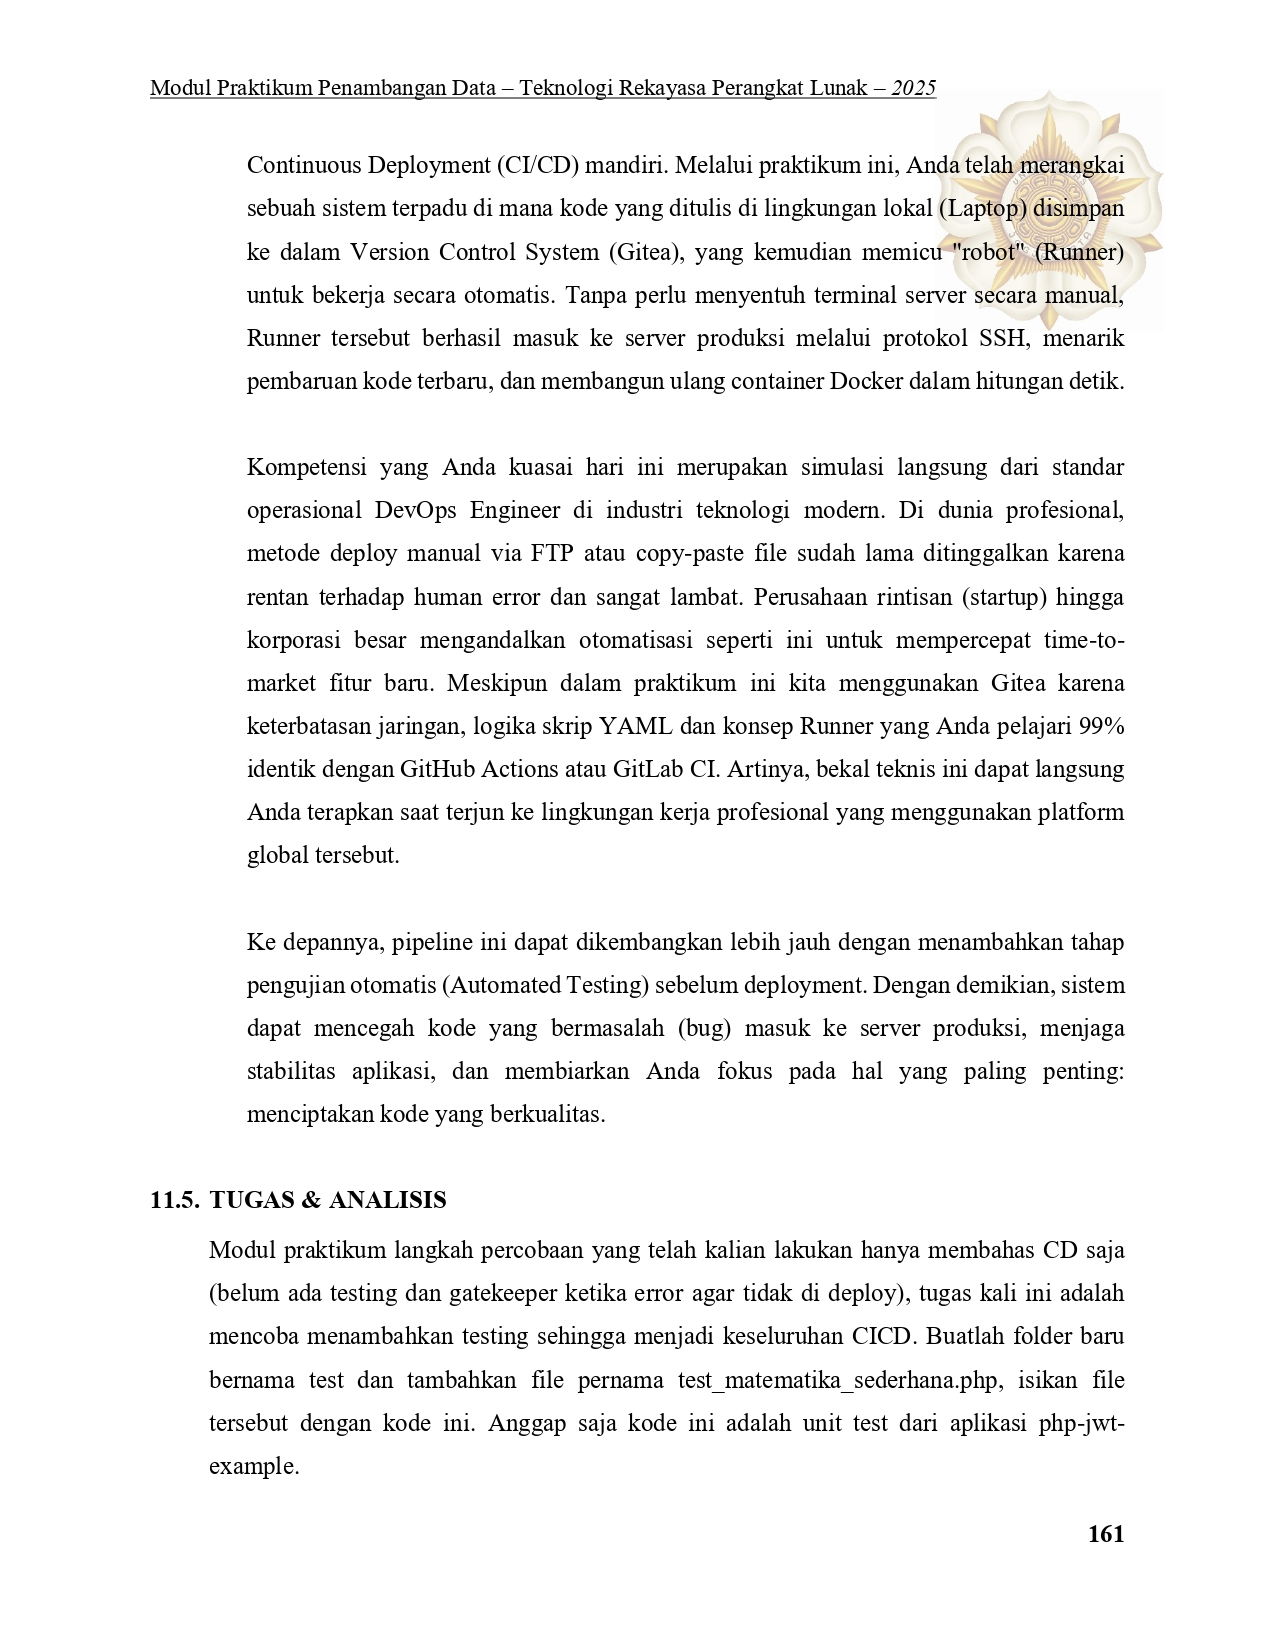
\includegraphics[width=0.95\textwidth]{resource/modul/Modul Praktikum Sistem Administrasi dan Informasi Terdistribusi 2026 v3_page-0161.jpg}
  \caption{Instruksi tugas pada modul praktikum - 1}
  \label{fig:p11-modul-161}
\end{figure}

\begin{figure}[H]
  \centering
  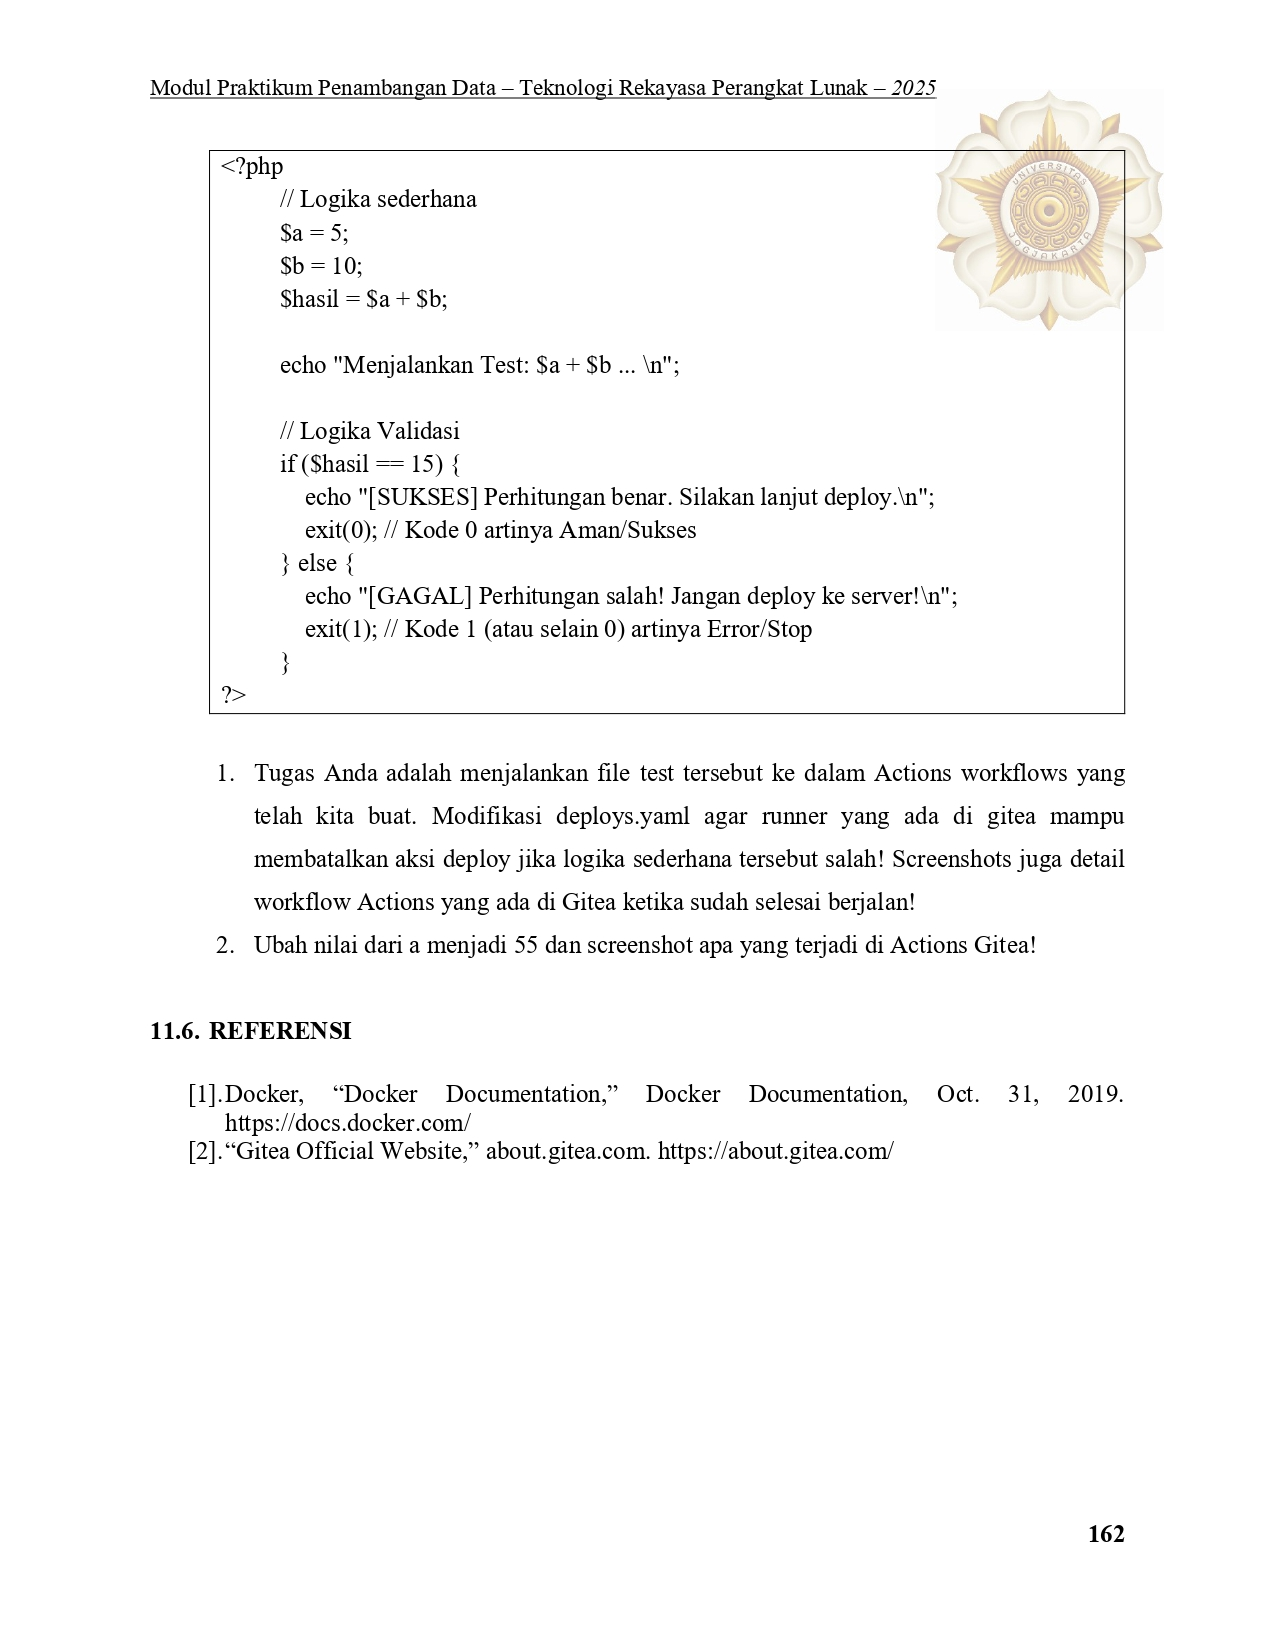
\includegraphics[width=0.95\textwidth]{resource/modul/Modul Praktikum Sistem Administrasi dan Informasi Terdistribusi 2026 v3_page-0162.jpg}
  \caption{Instruksi tugas pada modul praktikum - 2}
  \label{fig:p11-modul-162}
\end{figure}

\subsection{Perubahan Docker Compose untuk Deployment Aplikasi}

\par Aplikasi yang digunakan sebagai objek deployment adalah REST API JWT dari pertemuan sebelumnya. Pada tahap ini saya melakukan beberapa penyesuaian pada aplikasi agar lebih sesuai dengan proses deployment yang akan dilakukan melalui Gitea Actions. Penyesuaian tersebut meliputi penyederhanaan konfigurasi Docker Compose dan penyesuaian variabel environment untuk koneksi database MySQL yang sudah berjalan di VPS.

\par Perubahan yang saya lakukan adalah menyederhanakan stack Docker Compose pada versi baru. Pada kode lama, file \texttt{docker-compose.yml} menjalankan tiga service sekaligus (\texttt{be-jwt}, \texttt{database\_mysql}, dan \texttt{phpmyadmin}) serta menggunakan \texttt{depends\_on} untuk memastikan service API menunggu database. Pada versi baru, service database dan phpMyAdmin dikomentari karena database MySQL sudah berjalan sebagai service terpisah di VPS, sehingga proses deployment cukup fokus pada rebuild dan restart service API. Proses penyederhanaan ini ditunjukkan pada Gambar \ref{fig:p11-01-compose-comment}.

\begin{figure}[H]
  \centering
  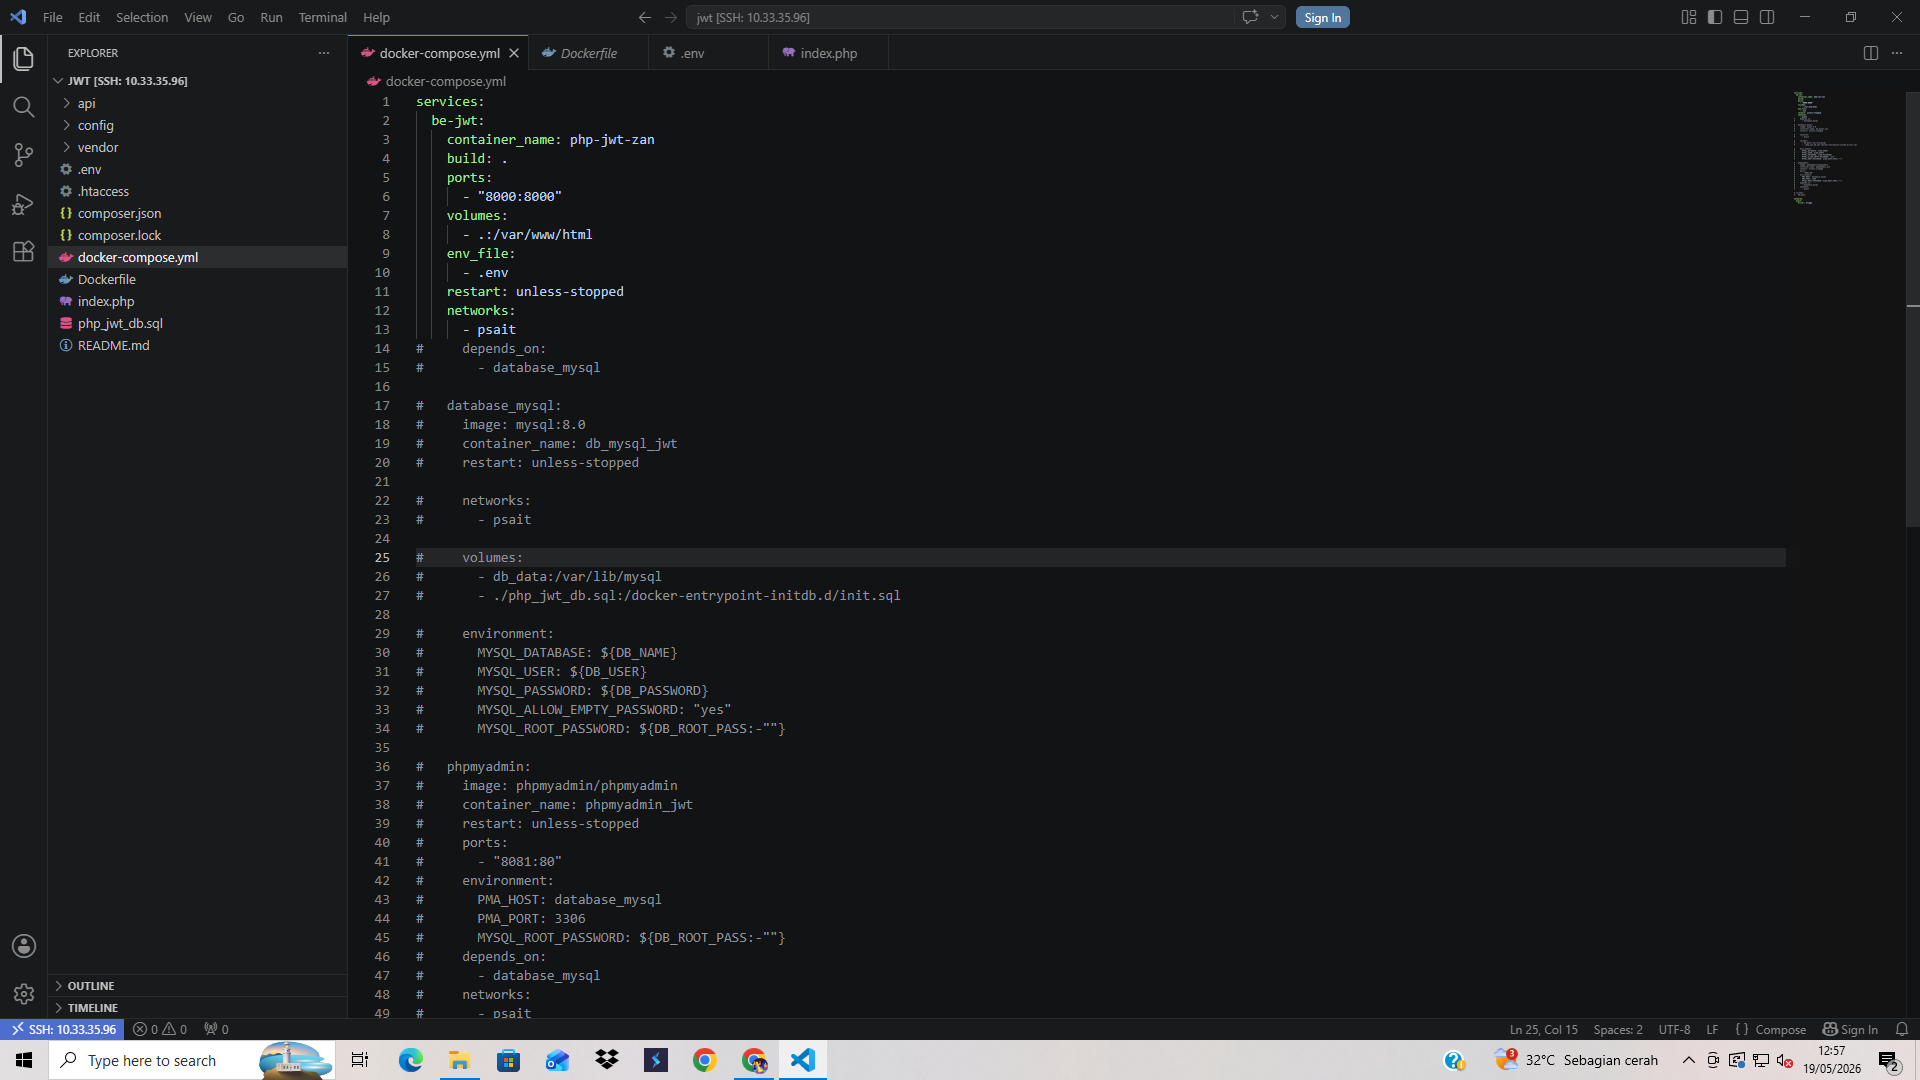
\includegraphics[width=0.95\textwidth]{resource/dokumentasi/1 - Edit file docker compose yml dengan mencoment beberapa baeis yang tidak diperlukan.png}
  \caption{Menyederhanakan \texttt{docker-compose.yml} dengan mengomentari service yang tidak diperlukan}
  \label{fig:p11-01-compose-comment}
\end{figure}

\par Perbandingan konfigurasi \texttt{docker-compose.yml} pada kode lama dan kode baru dirangkum pada Kode \ref{lst:p11-compose-old} dan Kode \ref{lst:p11-compose-new}.

\lstinputlisting[caption={Konfigurasi \texttt{docker-compose.yml} pada kode lama}, label={lst:p11-compose-old}]{resource/code/kodelama/docker-compose.yml}

\lstinputlisting[caption={Konfigurasi \texttt{docker-compose.yml} pada kode baru}, label={lst:p11-compose-new}]{resource/code/kodebaru/docker-compose.yml}

\par Terlihat bahwa pada kode baru, service \texttt{database\_mysql} dan \texttt{phpmyadmin} dikomentari, sehingga hanya service \texttt{be-jwt} yang akan dijalankan. Hal ini memungkinkan proses deployment menjadi lebih sederhana dan fokus pada aplikasi API saja, sementara database MySQL tetap berjalan secara terpisah di VPS.

\subsection{Menyiapkan Environment MySQL pada Host}

\par Karena service database MySQL telah dipisahkan dari \texttt{docker-compose.yml} milik aplikasi API, maka saya perlu memastikan bahwa MySQL pada VPS dapat diakses. Langkah yang dilakukan adalah dengan mengubah variabel environment host database agar mengarah langsung ke VPS dan mengecek status service MySQL tersebut. Proses ini ditunjukkan pada Gambar \ref{fig:p11-02-env-mysql} dan Gambar \ref{fig:p11-03-status-mysql}.

\par Perubahannya sebagai berikut pada listing \ref{lst:p11-check-mysql}, di mana nilai \texttt{DB\_HOST} diubah menjadi alamat IP VPS, sehingga aplikasi API nantinya akan terhubung ke MySQL yang berjalan di VPS.

\begin{lstlisting}[caption={Konfigurasi variabel environment database pada file \texttt{.env}}, label={lst:p11-check-mysql}]
DB_HOST=http://10.33.35.96 # Sebelumnya database_mysql
DB_PORT=3306
DB_NAME=sait_db
DB_USER=fauzan
DB_PASSWORD=fauzan123
\end{lstlisting}

\begin{figure}[H]
  \centering
  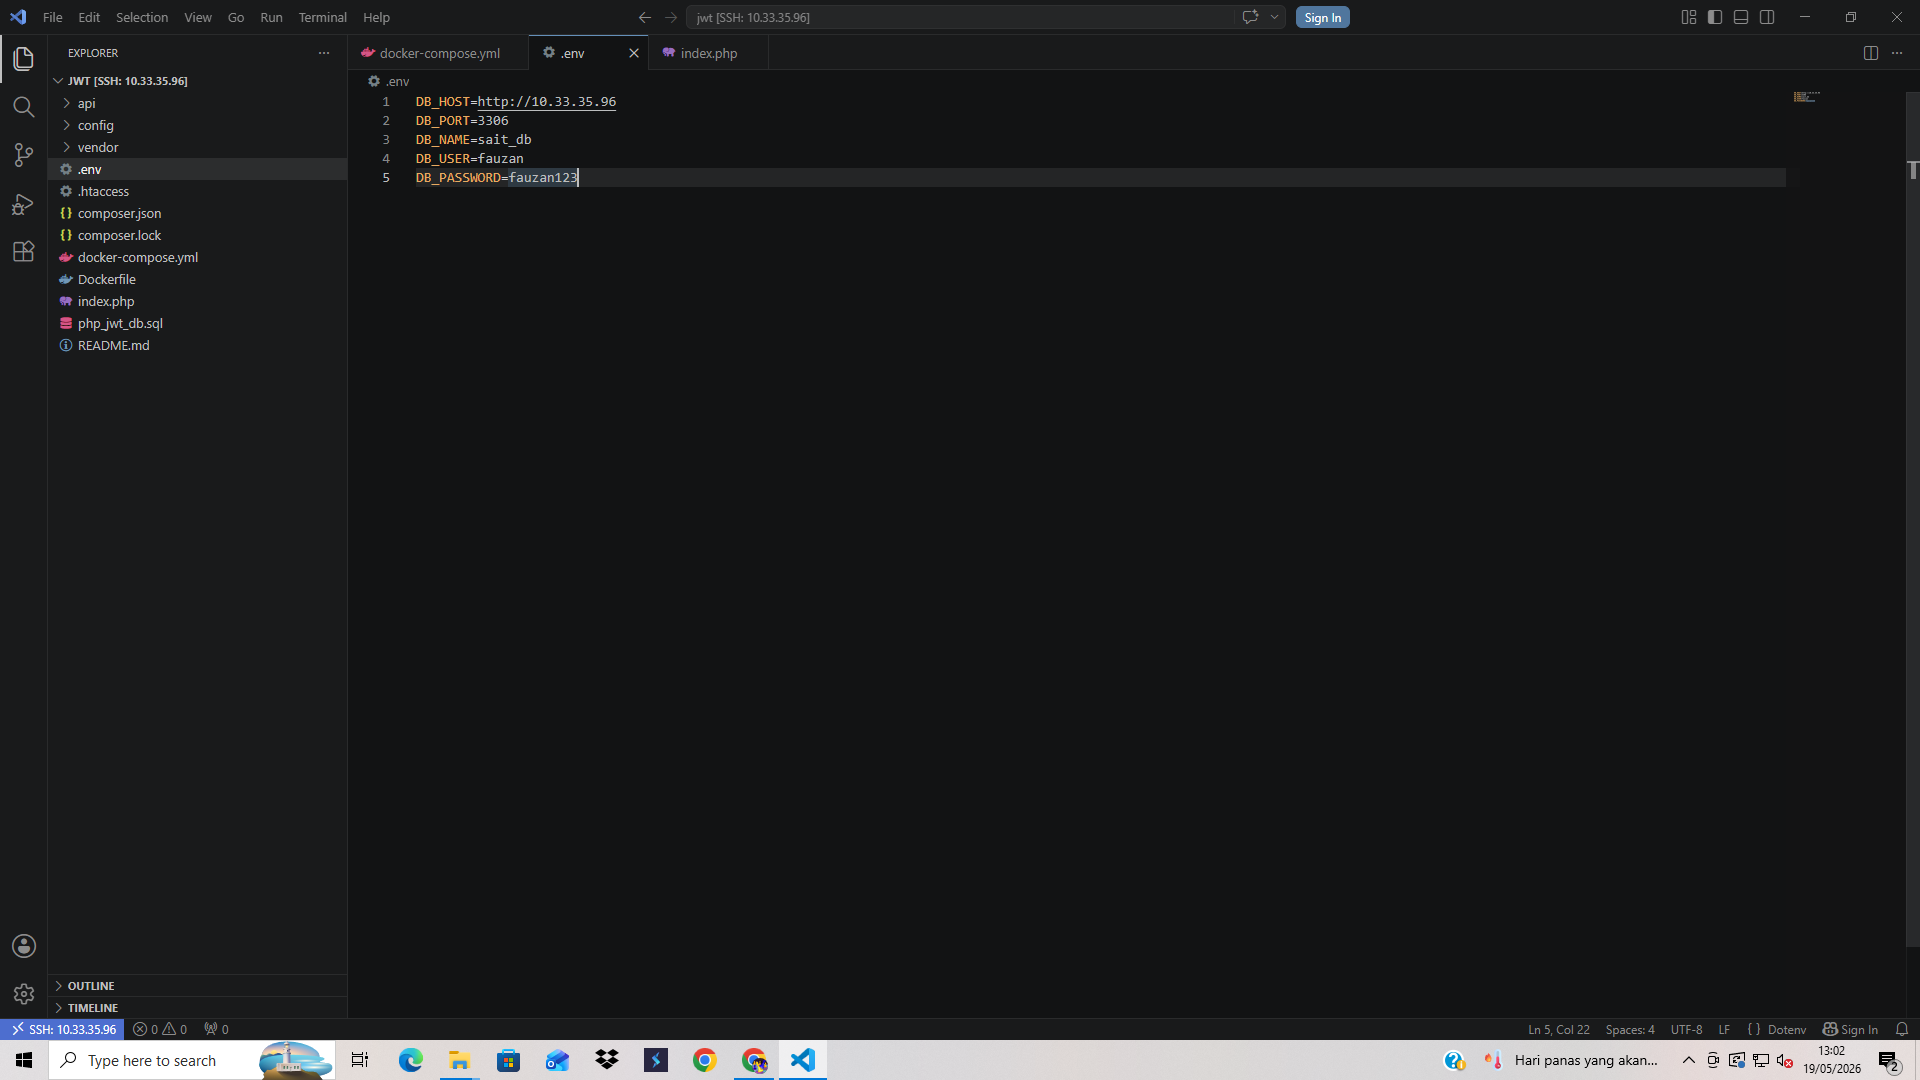
\includegraphics[width=0.95\textwidth]{resource/dokumentasi/2 - Ganti Env untuk mysql ke server.png}
  \caption{Mengubah file \texttt{.env} agar \texttt{DB\_HOST} menggunakan alamat VPS}
  \label{fig:p11-02-env-mysql}
\end{figure}

\par Terlihat pada Gambar \ref{fig:p11-02-env-mysql} bahwa nilai \texttt{DB\_HOST} diubah menjadi alamat IP VPS, sehingga aplikasi API nantinya akan terhubung ke MySQL yang berjalan di VPS. Setelah perubahan ini dilakukan, saya menjalankan perintah untuk mengecek status layanan MySQL di VPS guna memastikan bahwa layanan tersebut aktif dan siap menerima koneksi (Gambar \ref{fig:p11-03-status-mysql}).

\begin{figure}[H]
  \centering
  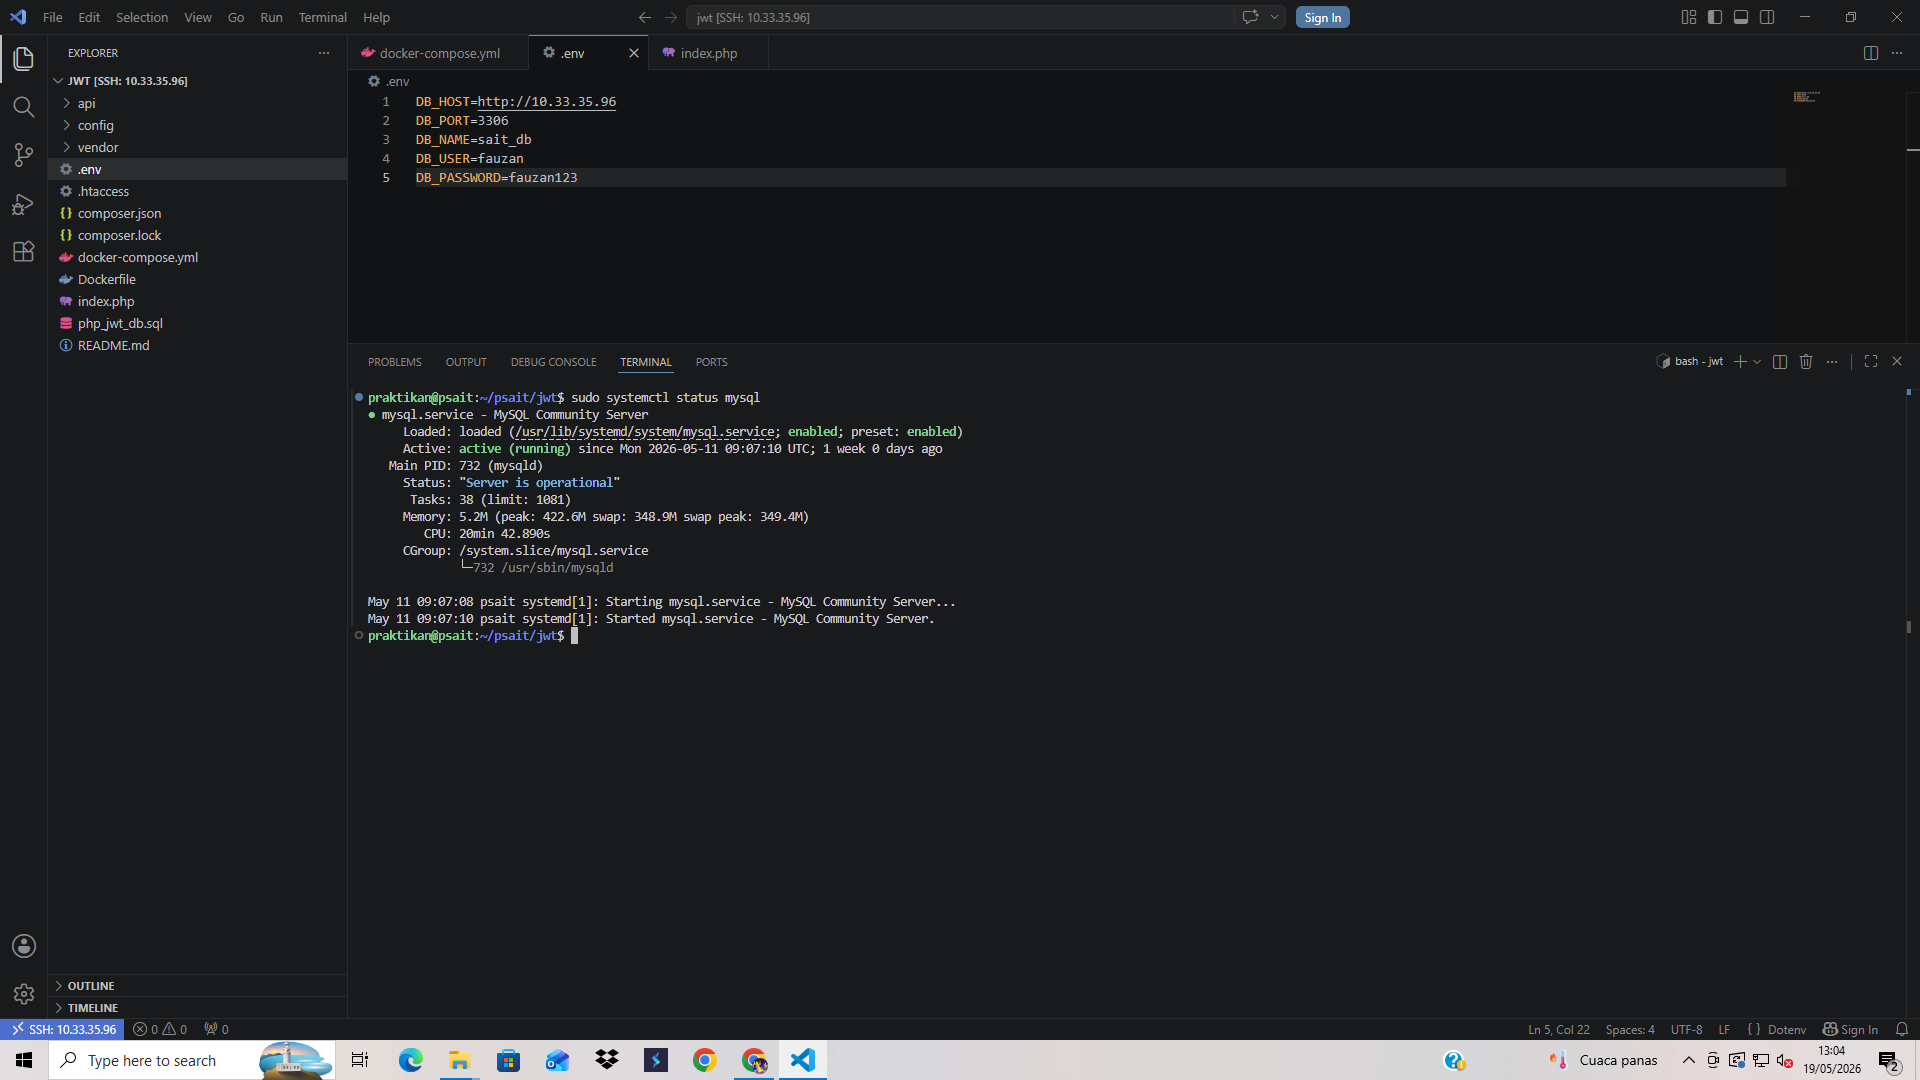
\includegraphics[width=0.95\textwidth]{resource/dokumentasi/3 - Cek status mysql.png}
  \caption{Mengecek status layanan MySQL di server VPS}
  \label{fig:p11-03-status-mysql}
\end{figure}

\par Terlihat pada Gambar \ref{fig:p11-03-status-mysql} bahwa layanan MySQL sedang berjalan dengan status \texttt{active (running)}, sehingga siap digunakan sebagai database untuk aplikasi API yang akan dideploy melalui Gitea Actions.

\subsection{Instalasi Gitea menggunakan Docker Compose di VPS}

\par Setelah aplikasi siap, langkah selanjutnya adalah menyiapkan infrastruktur CI/CD menggunakan Gitea. Gitea merupakan layanan Git \textit{self-hosted} yang ringan dan mudah dijalankan melalui Docker. Di server VPS, saya membuat direktori kerja khusus untuk Gitea (Gambar \ref{fig:p11-04-folder-gitea}). Perintah pembuatan direktori dan perpindahan direktori ditunjukkan pada Listing \ref{lst:p11-mkdir-gitea}.

\begin{lstlisting}[caption={Membuat direktori kerja Gitea di VPS}, label={lst:p11-mkdir-gitea}]
mkdir gitea
cd gitea
\end{lstlisting}

\par Setelah berada di dalam direktori tersebut, saya membuat file \texttt{docker-compose.yml} untuk menjalankan service Gitea (Gambar \ref{fig:p11-05-compose-gitea}). Secara garis besar, konfigurasi tersebut menjalankan container Gitea pada port web \texttt{3000} dan port SSH pada \texttt{222}, serta menyimpan data persistent pada volume lokal. Konfigurasi \texttt{docker-compose.yml} yang digunakan ditunjukkan pada Listing \ref{lst:p11-compose-gitea}.

\begin{lstlisting}[caption={Konfigurasi Docker Compose untuk service Gitea}, label={lst:p11-compose-gitea}]
version: "3.8"

networks:
  gitea:
    external: false

services:
  server:
    image: docker.gitea.com/gitea:1.25.3
    container_name: gitea
    restart: always
    environment:
      - USER_UID=1000
      - USER_GID=1000
      - HTTP_LISTEN=0.0.0.0
    networks:
      - gitea
    volumes:
      - ./gitea:/data
      - /etc/timezone:/etc/timezone:ro
      - /etc/localtime:/etc/localtime:ro
    ports:
      - "3000:3000"
      - "222:22"
\end{lstlisting}

\begin{figure}[H]
  \centering
  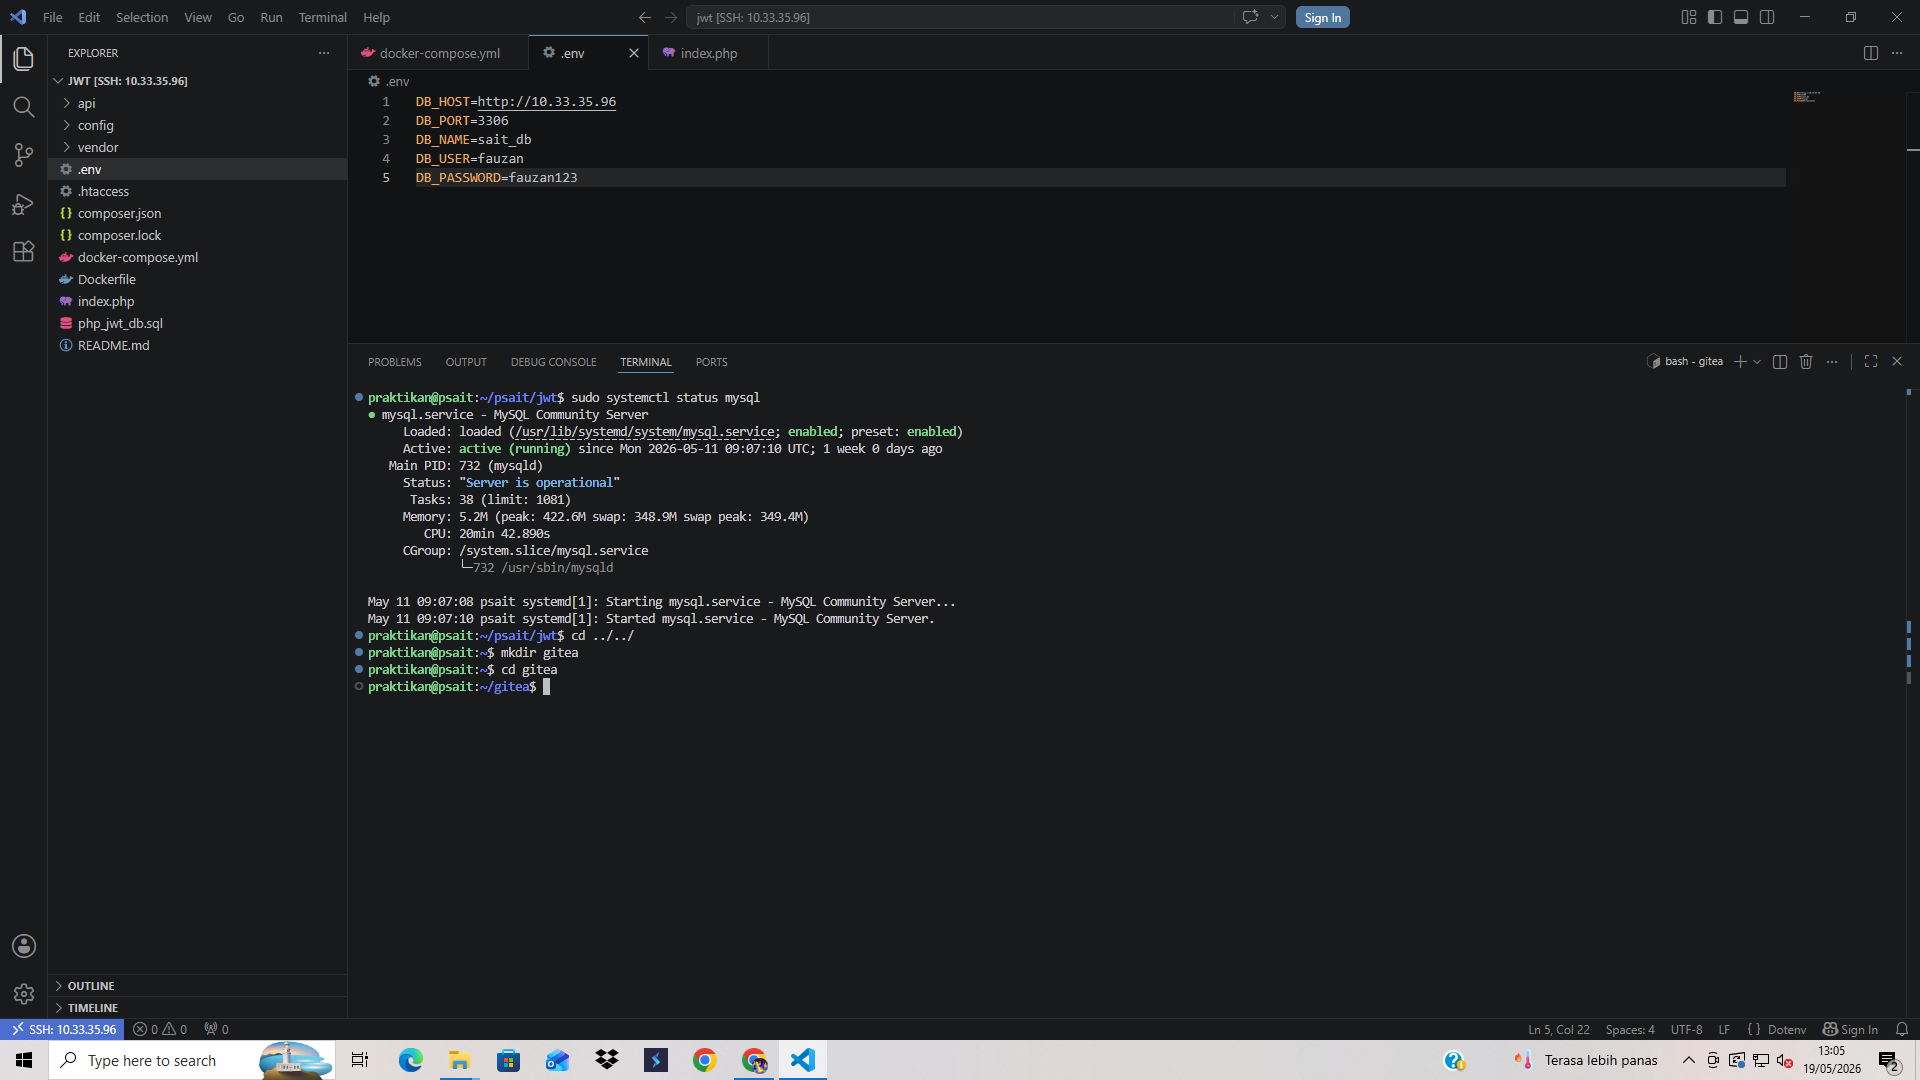
\includegraphics[width=0.95\textwidth]{resource/dokumentasi/4 - Buat folder gitea.png}
  \caption{Membuat direktori khusus untuk Gitea di VPS}
  \label{fig:p11-04-folder-gitea}
\end{figure}

\begin{figure}[H]
  \centering
  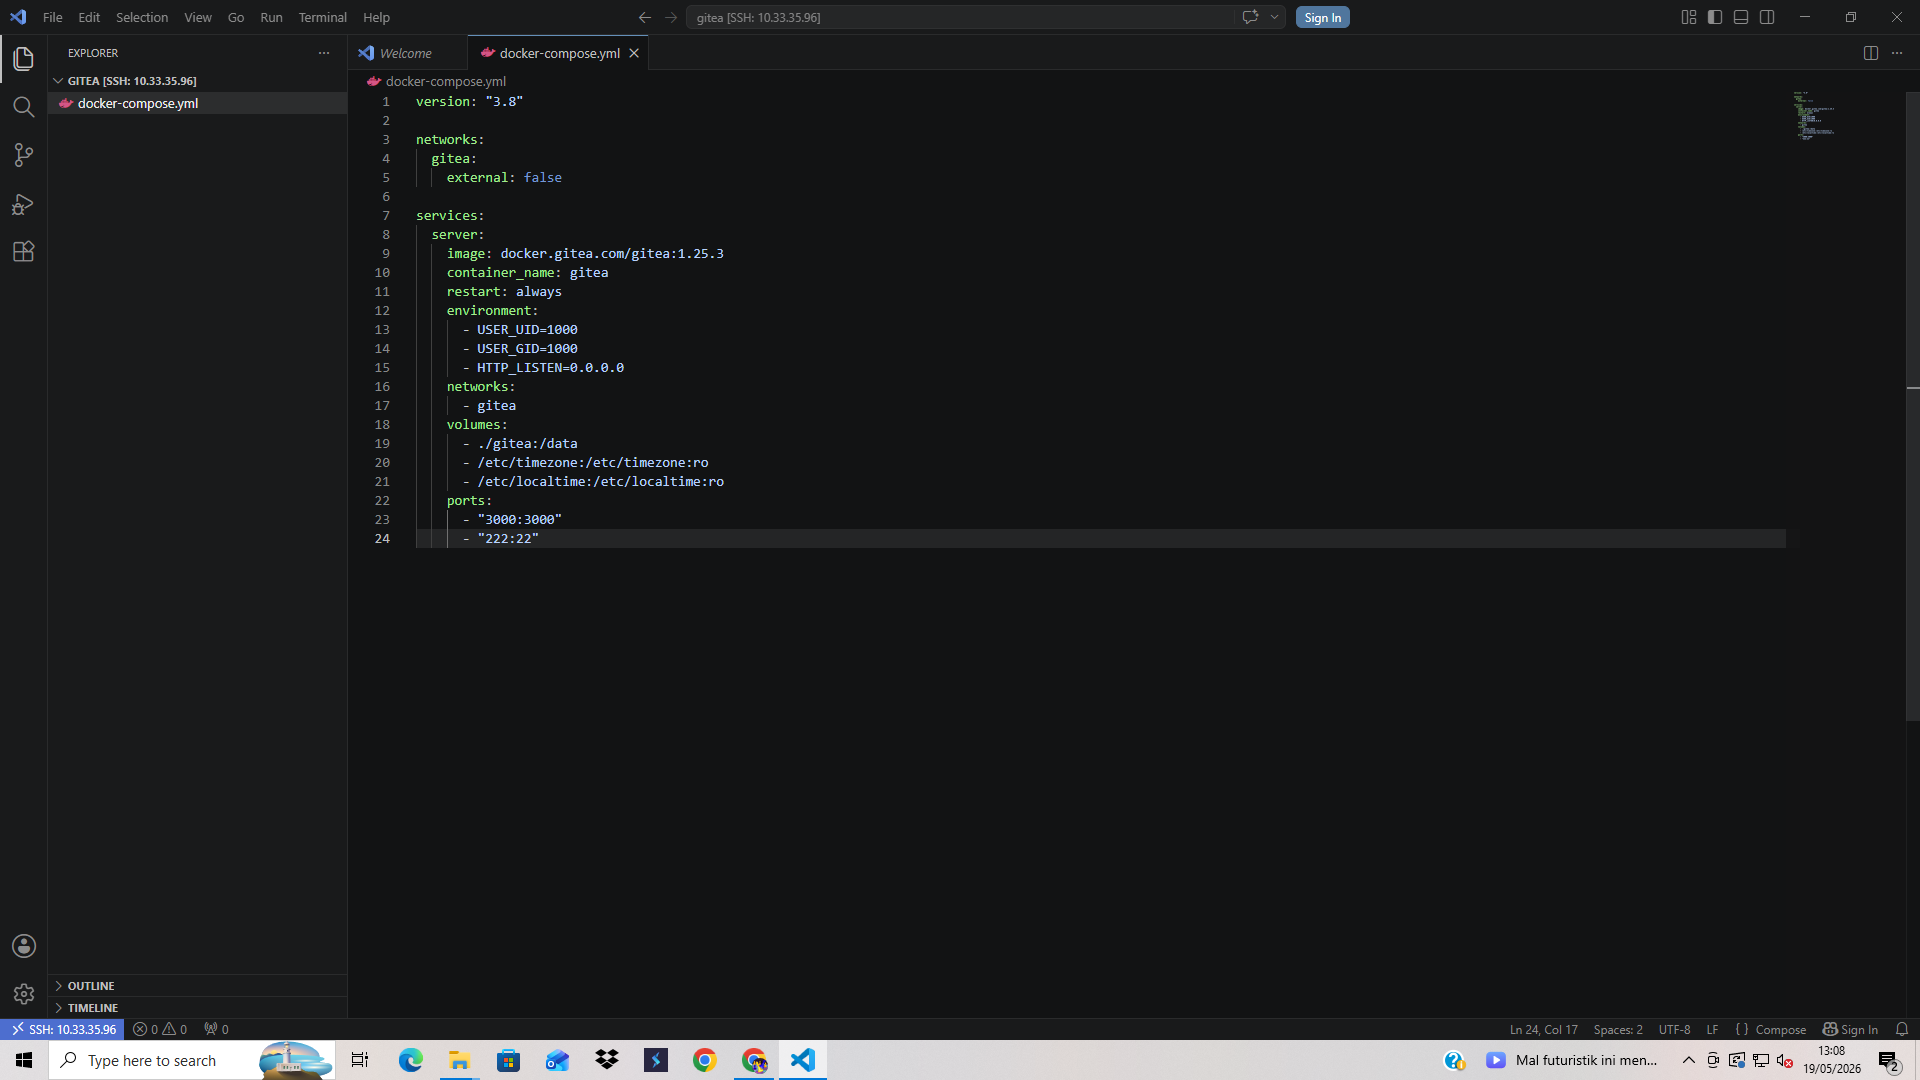
\includegraphics[width=0.95\textwidth]{resource/dokumentasi/5 - Buat docker compose yml di folder gitea.png}
  \caption{Membuat konfigurasi \texttt{docker-compose.yml} untuk menjalankan Gitea}
  \label{fig:p11-05-compose-gitea}
\end{figure}

\par Setelah file \texttt{docker-compose.yml} dibuat, layanan Gitea dijalankan menggunakan perintah \texttt{docker compose up -d} (Gambar \ref{fig:p11-06-gitea-up}). Perintah untuk menjalankan service ditunjukkan pada Listing \ref{lst:p11-compose-up-gitea}.

\begin{lstlisting}[caption={Menjalankan container Gitea dengan Docker Compose}, label={lst:p11-compose-up-gitea}]
docker compose up -d
\end{lstlisting}

\par Layanan Gitea kemudian diakses melalui web browser menggunakan alamat ip vps dengan format \texttt{http://<IP-VPS>:3000}. Pada halaman awal, saya melakukan konfigurasi instalasi dasar Gitea (Gambar \ref{fig:p11-07-install-gitea}) dan dilanjutkan dengan pendaftaran akun administrator baru (Gambar \ref{fig:p11-08-register-gitea}). Setelah seluruh konfigurasi awal selesai, dashboard utama Gitea akan tampil dan siap digunakan (Gambar \ref{fig:p11-09-dashboard-gitea}).

\begin{figure}[H]
  \centering
  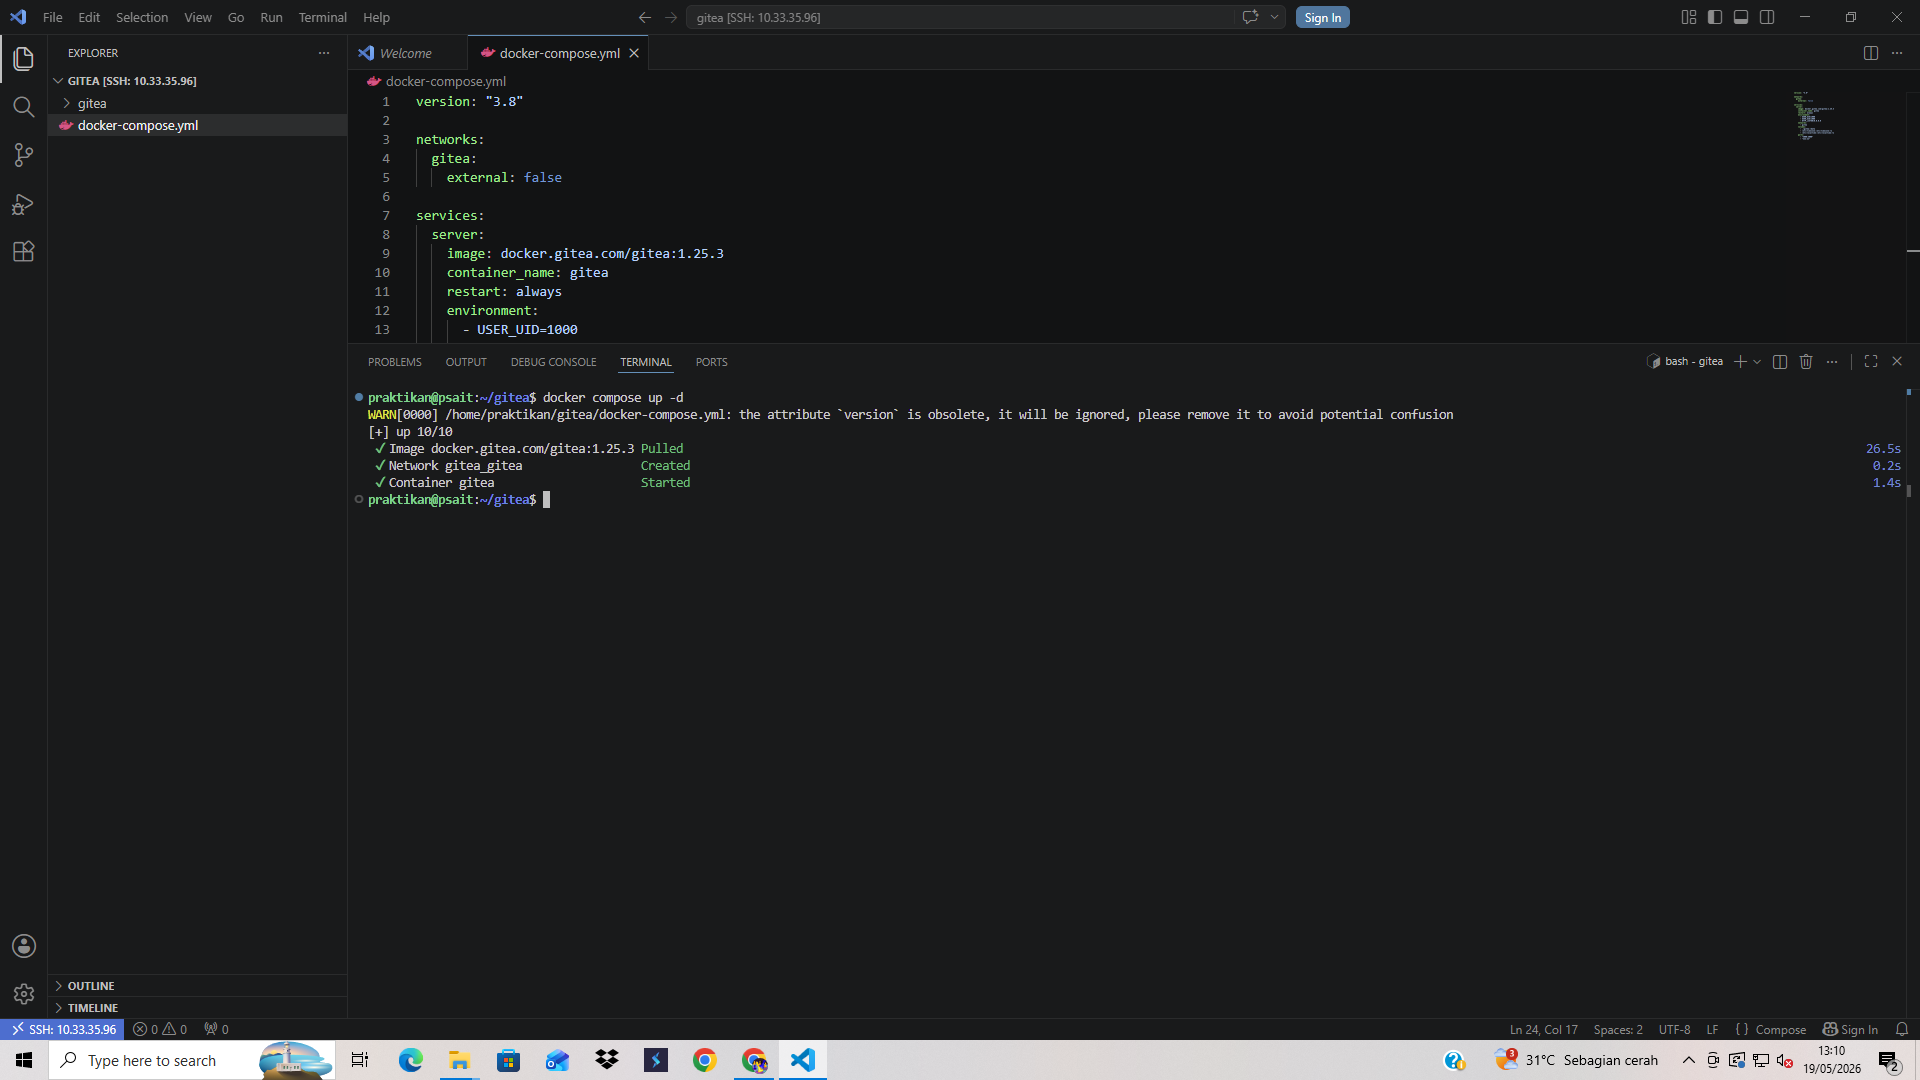
\includegraphics[width=0.95\textwidth]{resource/dokumentasi/6 - Docker compose up.png}
  \caption{Menjalankan service Gitea menggunakan \texttt{docker compose up -d}}
  \label{fig:p11-06-gitea-up}
\end{figure}

\begin{figure}[H]
  \centering
  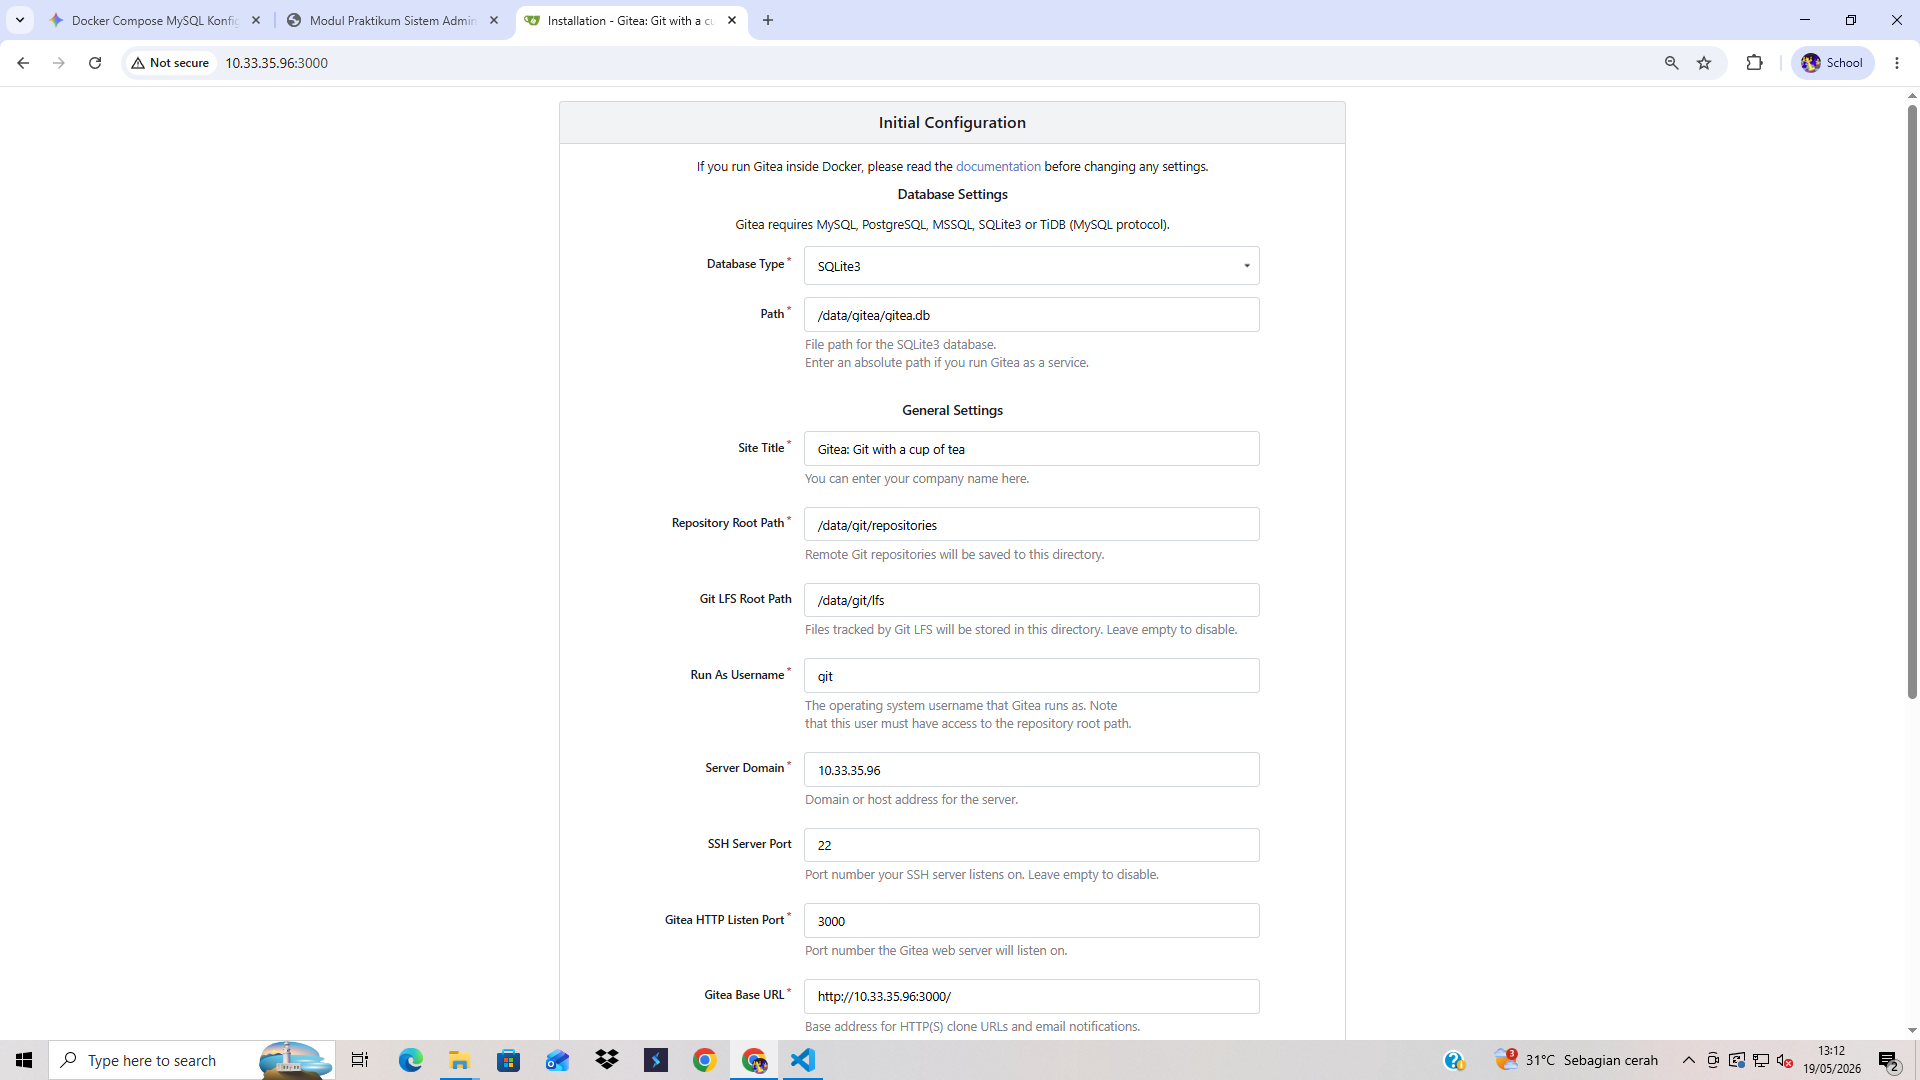
\includegraphics[width=0.95\textwidth]{resource/dokumentasi/7 - Tampilan isntalasi gitea.png}
  \caption{Halaman awal instalasi Gitea di browser}
  \label{fig:p11-07-install-gitea}
\end{figure}

\begin{figure}[H]
  \centering
  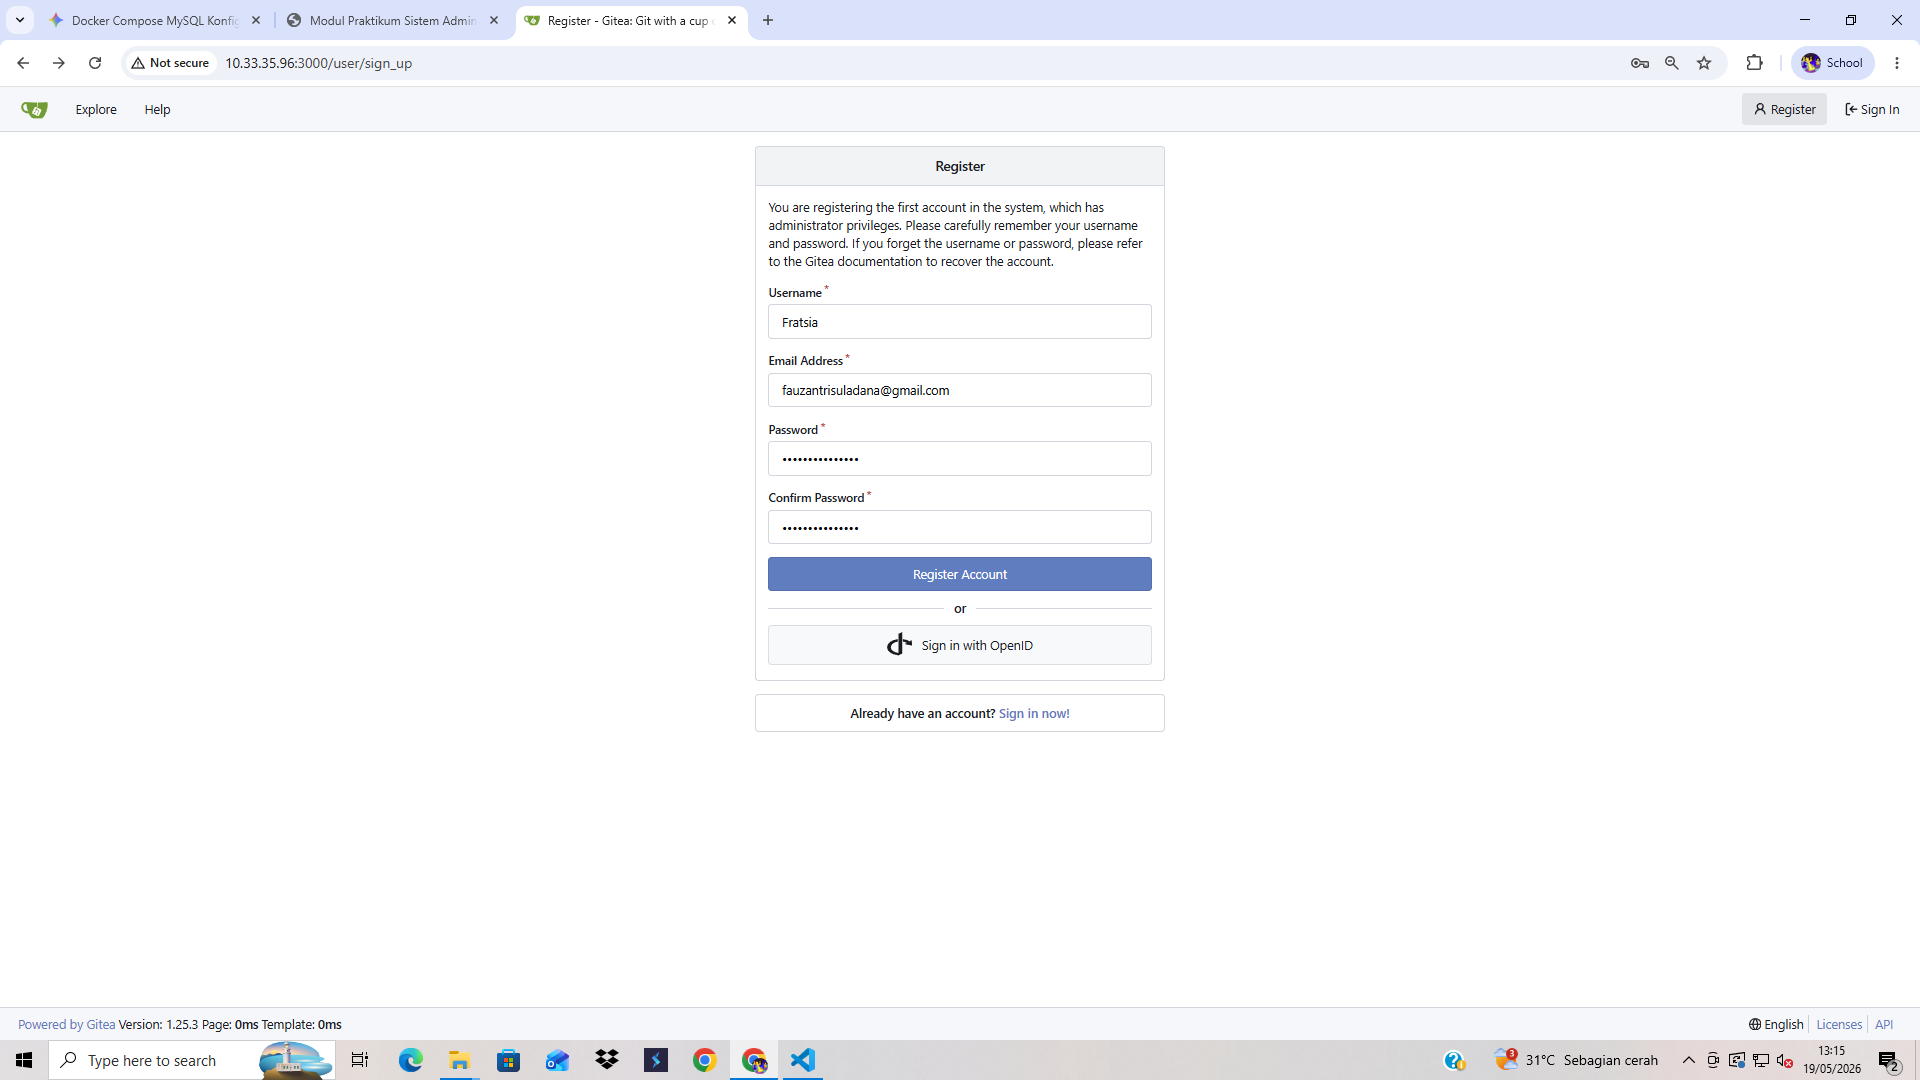
\includegraphics[width=0.95\textwidth]{resource/dokumentasi/8 - pendaftaran akun gitea.png}
  \caption{Pendaftaran akun administrator Gitea}
  \label{fig:p11-08-register-gitea}
\end{figure}

\par Setelah proses instalasi dan pendaftaran selesai, Gitea siap digunakan untuk menyimpan \textit{source code} aplikasi.

\begin{figure}[H]
  \centering
  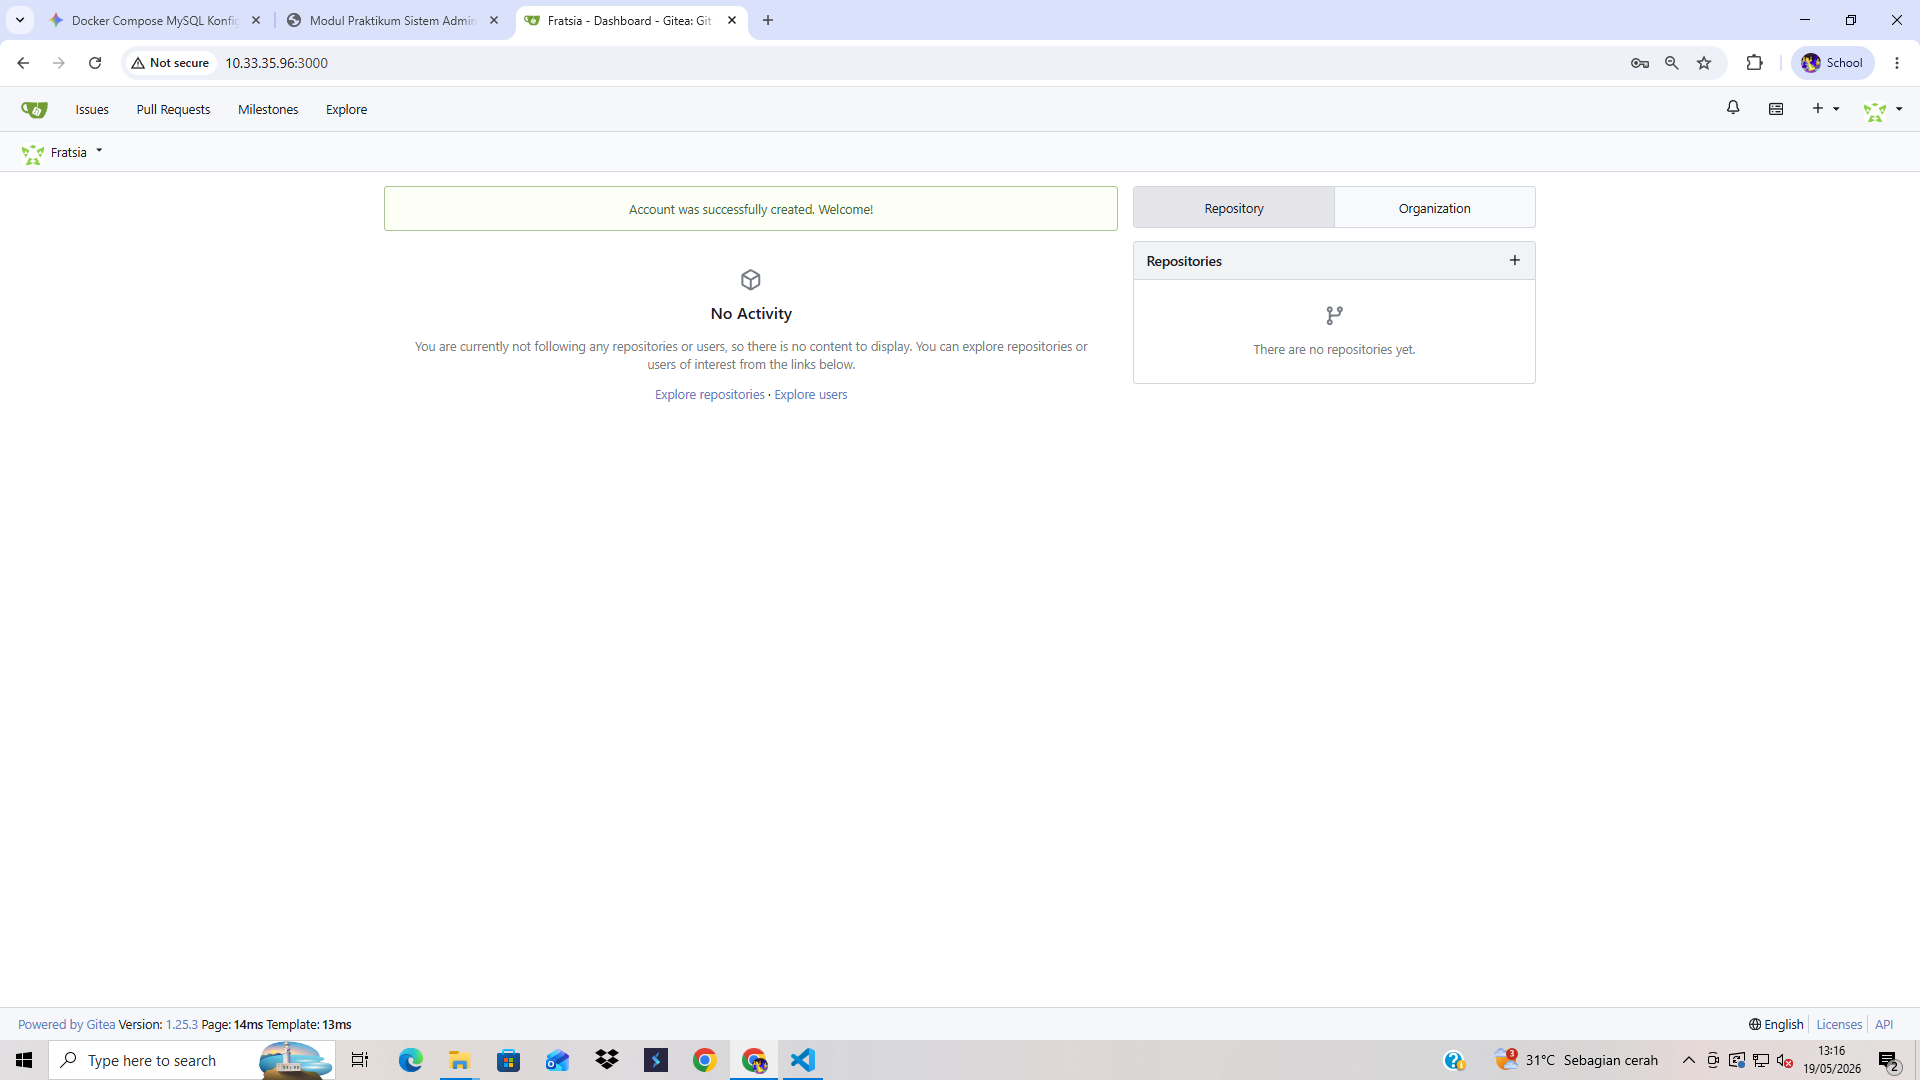
\includegraphics[width=0.95\textwidth]{resource/dokumentasi/9 - Halaman utama gitea.png}
  \caption{Halaman dashboard utama Gitea setelah login}
  \label{fig:p11-09-dashboard-gitea}
\end{figure}

\par Agar layanan Gitea dapat menjalankan workflow pipeline (Gitea Actions), diperlukan komponen tambahan berupa Gitea Runner. Pendaftaran runner baru dimulai dengan mengakses menu \textit{Site Administration} pada Gitea (Gambar \ref{fig:p11-10-site-admin}), kemudian membuka bagian \textit{Actions} $\rightarrow$ \textit{Runners} untuk membuat instance runner baru dan memperoleh \textit{registration token} (Gambar \ref{fig:p11-11-new-runner}).

\begin{figure}[H]
  \centering
  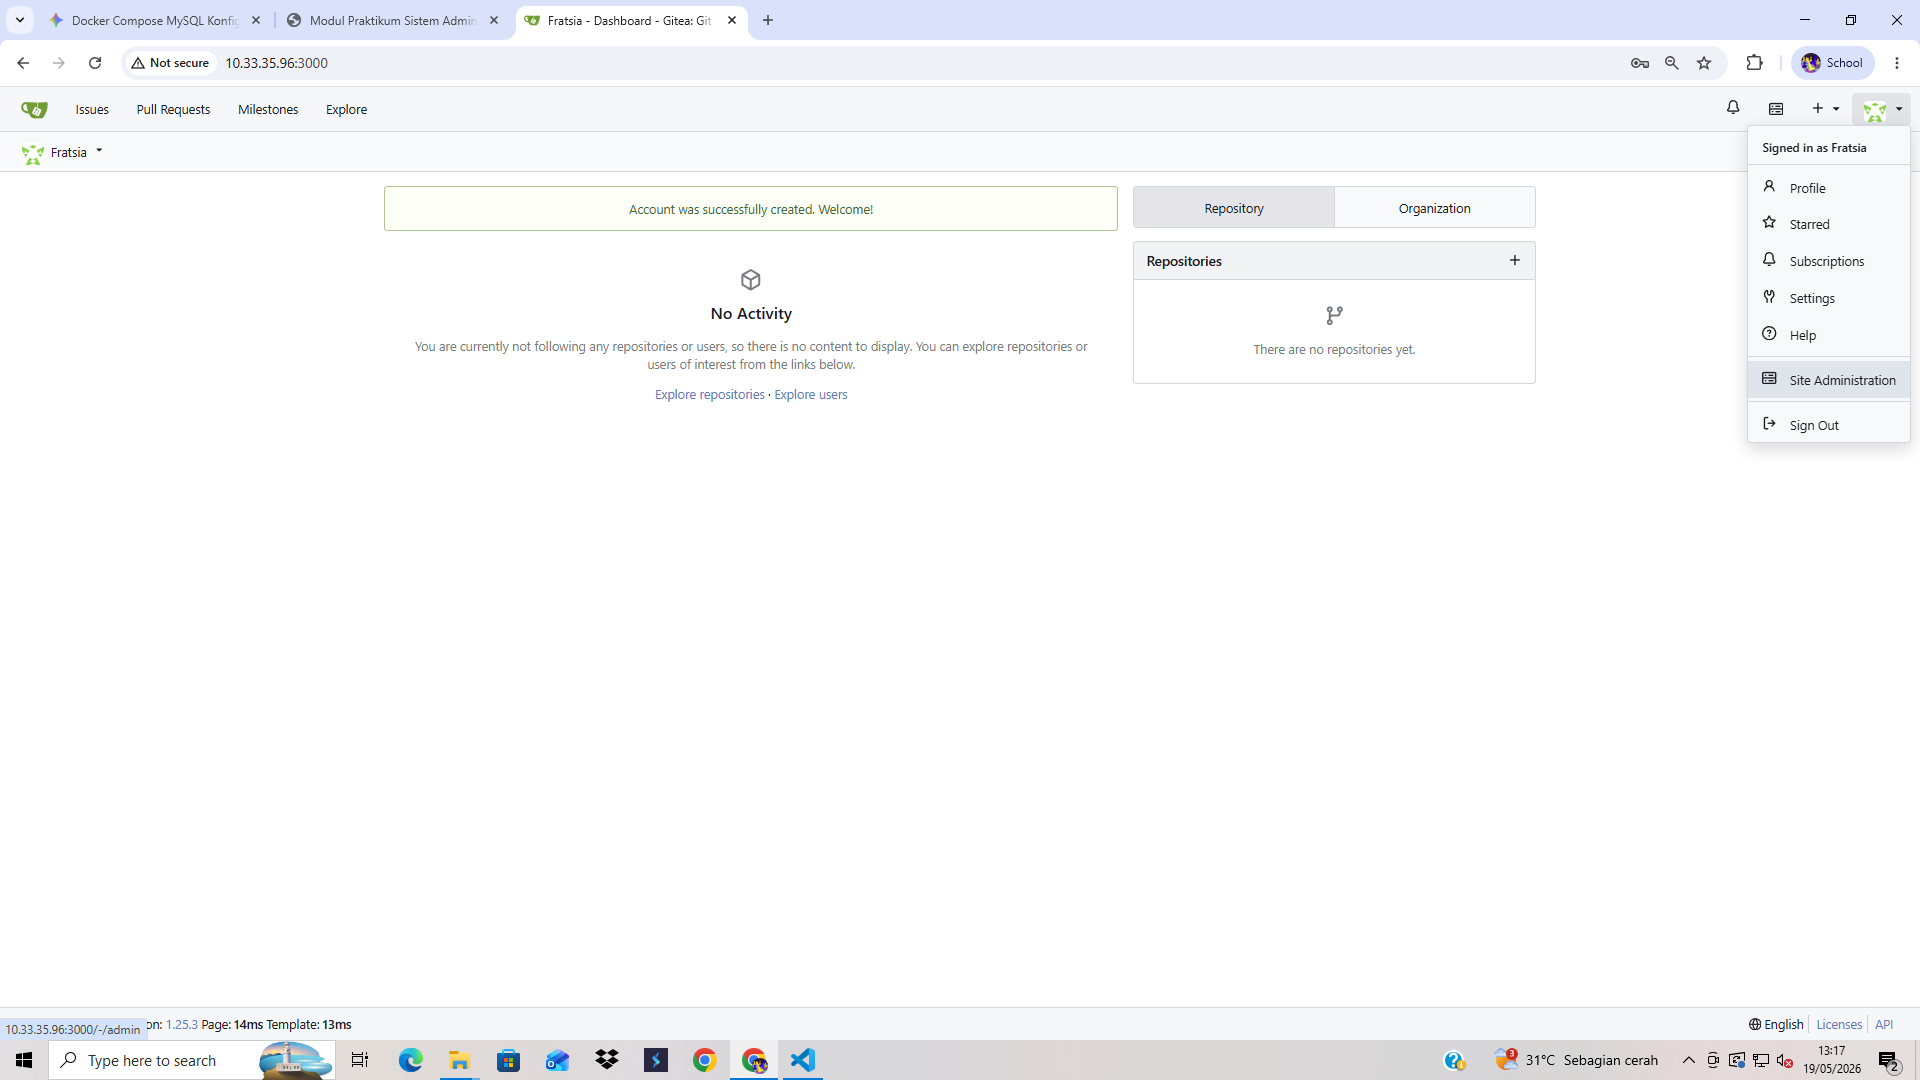
\includegraphics[width=0.95\textwidth]{resource/dokumentasi/10 - ke halaman site administration.png}
  \caption{Mengakses halaman Site Administration pada Gitea}
  \label{fig:p11-10-site-admin}
\end{figure}

\begin{figure}[H]
  \centering
  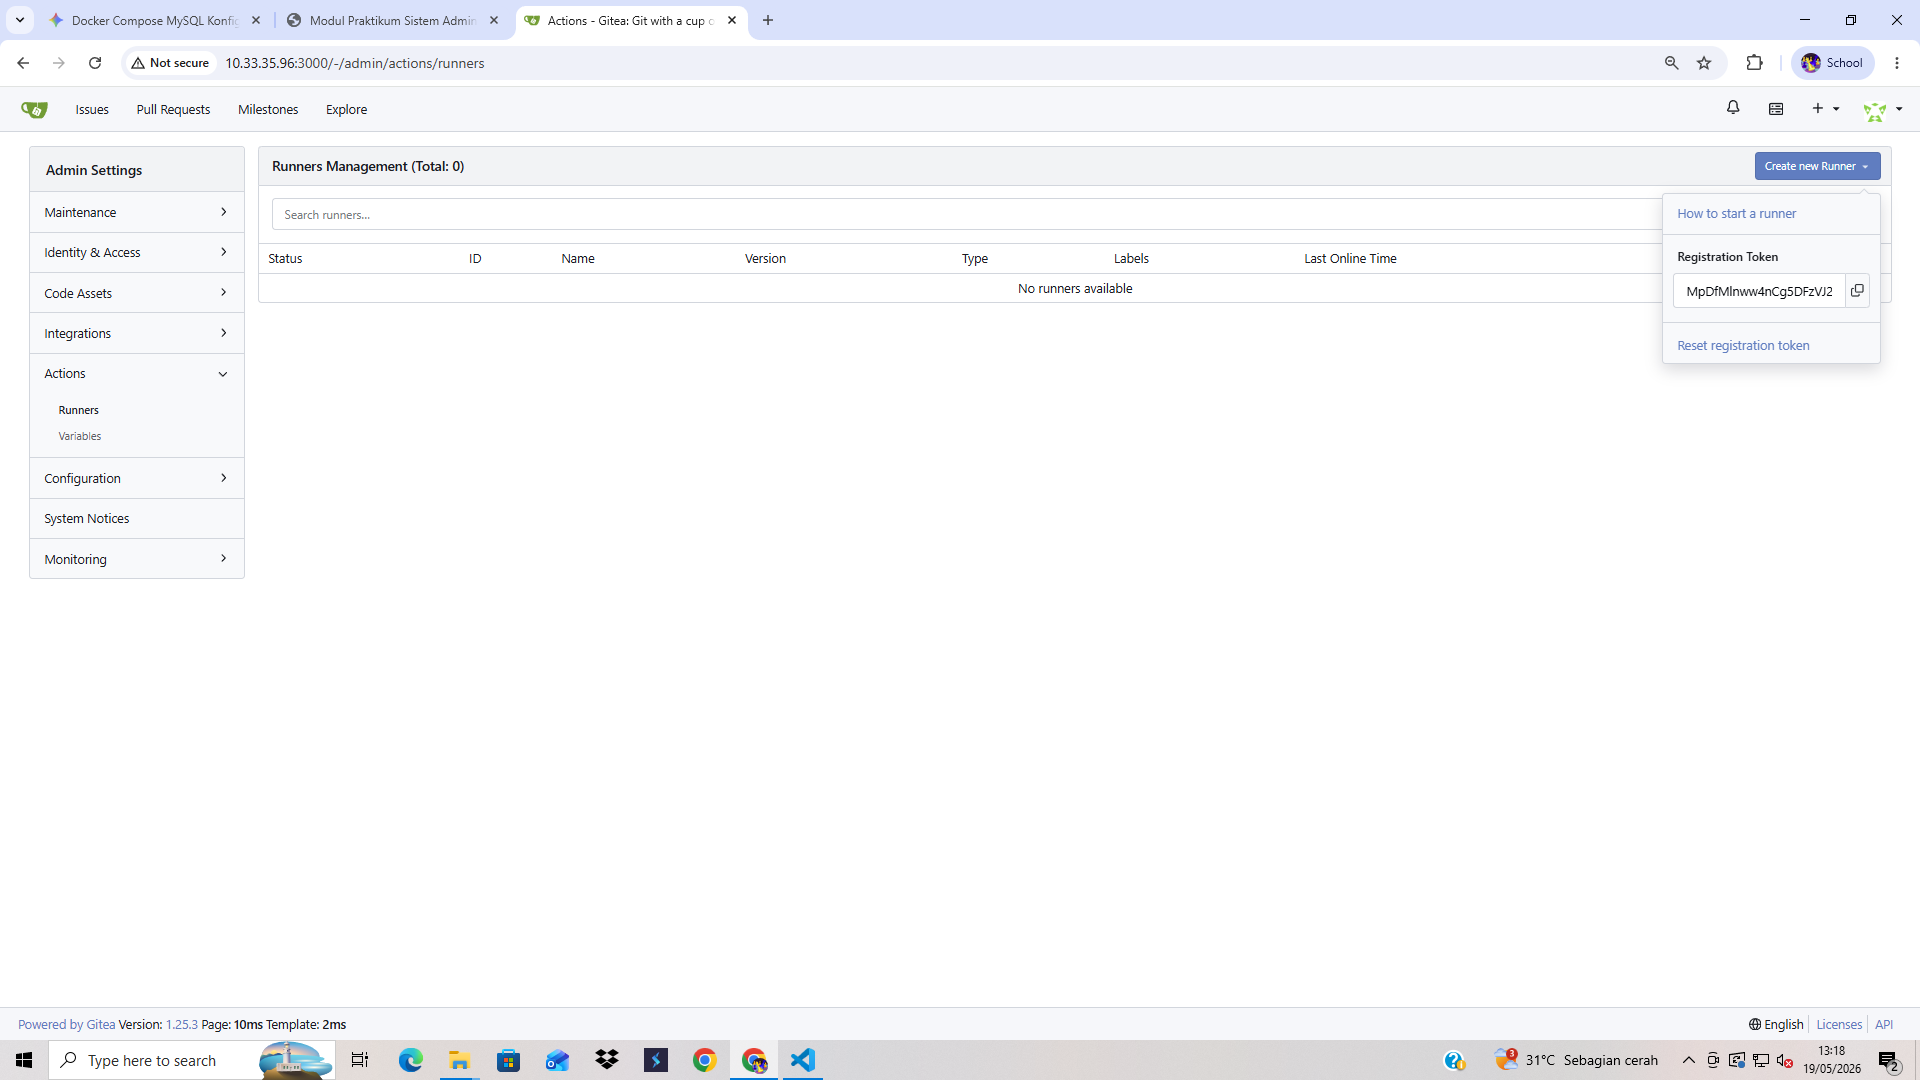
\includegraphics[width=0.95\textwidth]{resource/dokumentasi/11 - new runner.png}
  \caption{Membuat \textit{Runner} baru untuk mendapatkan token pendaftaran}
  \label{fig:p11-11-new-runner}
\end{figure}

\par Setelah registrasi token diperoleh, file \texttt{docker-compose.yml} milik Gitea dimodifikasi untuk menambahkan service runner baru dan mendefinisikan token tersebut sebagai salah satu \textit{environment variable} (Gambar \ref{fig:p11-12-modifikasi-compose}). Nilai token disamarkan menggunakan placeholder pada Listing \ref{lst:p11-compose-runner} untuk alasan keamanan data kredensial.

\begin{lstlisting}[caption={Menambahkan service runner pada Docker Compose (token disamarkan)}, label={lst:p11-compose-runner}]
runner:
  image: gitea/act_runner:latest
  container_name: gitea_runner
  restart: unless-stopped
  networks:
    - gitea
  depends_on:
    - server
  volumes:
    - /var/run/docker.sock:/var/run/docker.sock
    - ./runner-data:/data
  environment:
    - GITEA_INSTANCE_URL=http://gitea:3000
    - GITEA_RUNNER_REGISTRATION_TOKEN=<TOKEN_DARI_GITEA>
    - GITEA_RUNNER_NAME=jwt
    - GITEA_RUNNER_LABELS=ubuntu-latest:docker://node:16-alpine
\end{lstlisting}

\begin{figure}[H]
  \centering
  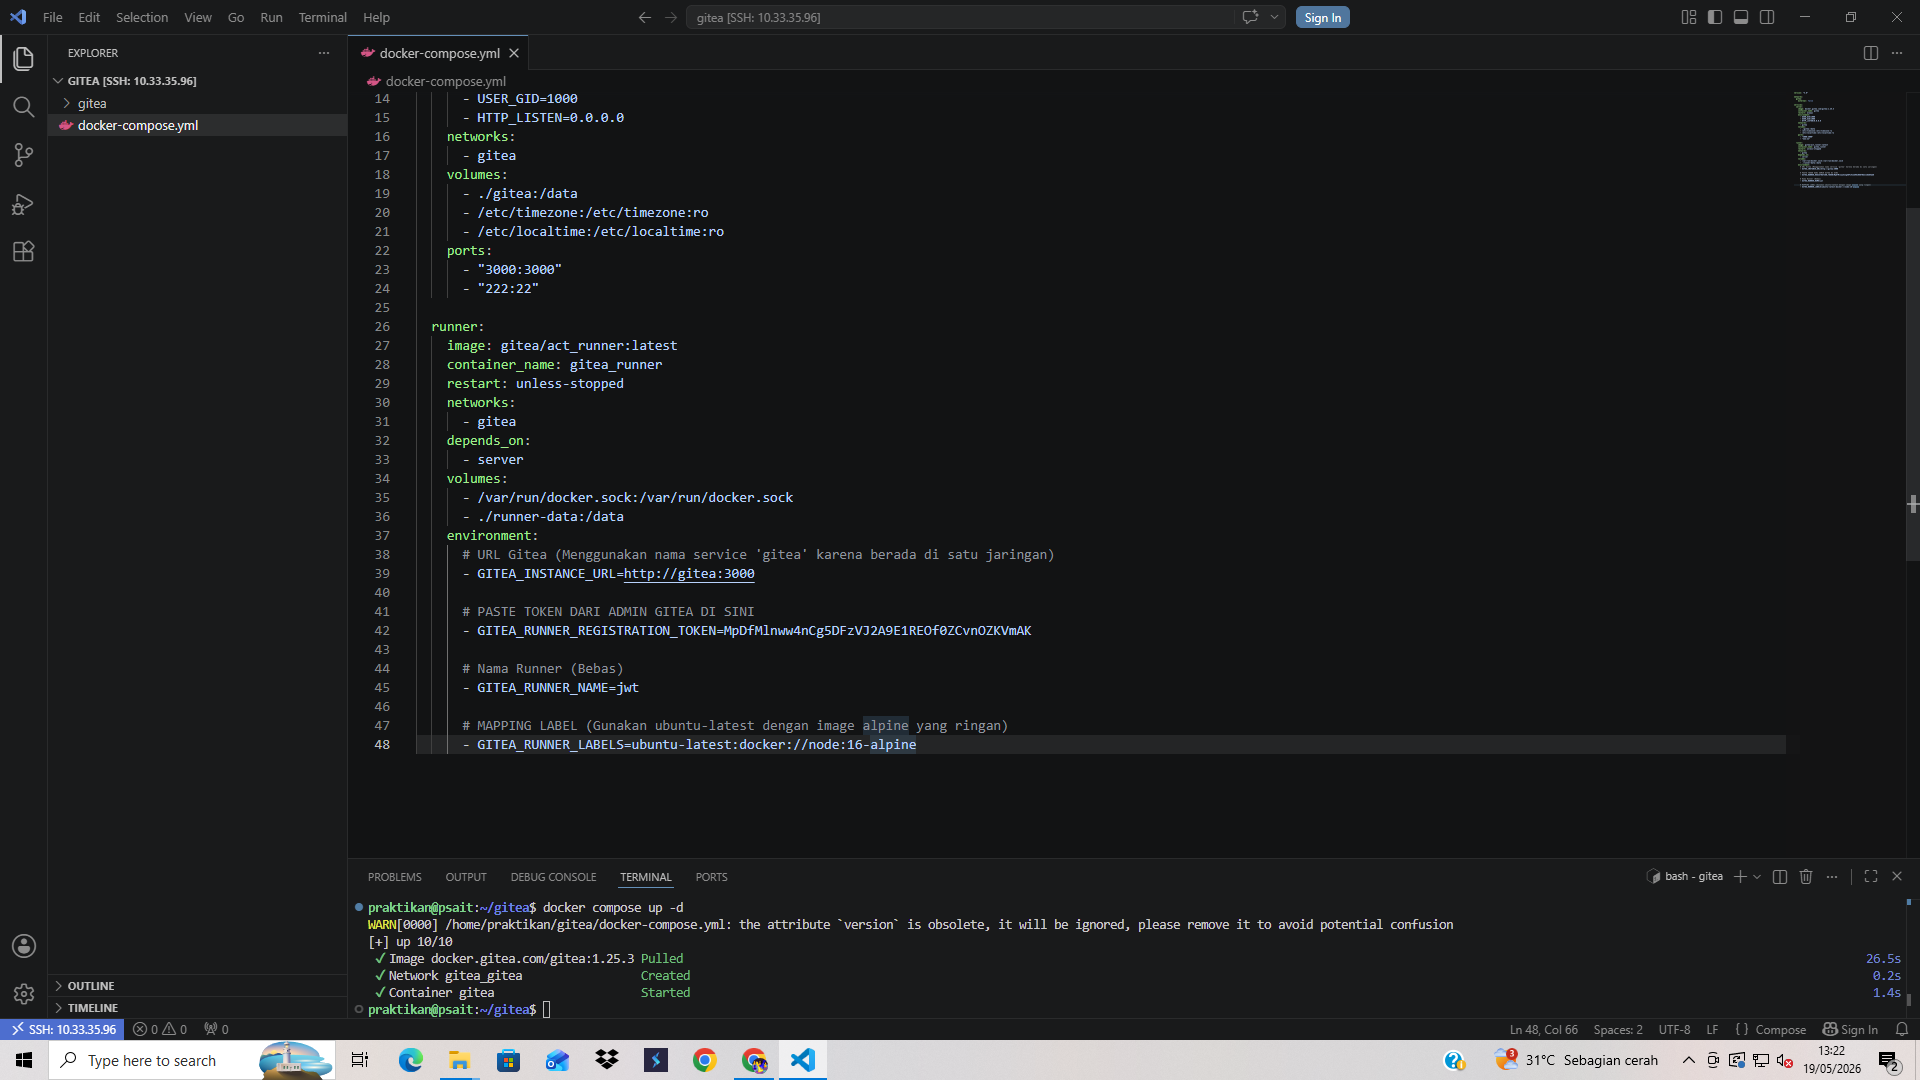
\includegraphics[width=0.95\textwidth]{resource/dokumentasi/12 - modifikasi docker compose yml.png}
  \caption{Menambahkan service \texttt{gitea-runner} pada \texttt{docker-compose.yml}}
  \label{fig:p11-12-modifikasi-compose}
\end{figure}

\par Selanjutnya, perintah \texttt{docker compose up -d} dijalankan kembali untuk menerapkan perubahan dan mengaktifkan service runner (Gambar \ref{fig:p11-13-runner-up}). Status koneksi runner diverifikasi melalui halaman administrator Gitea, yang menunjukkan bahwa runner telah aktif dengan status \textit{idle/online} dan siap menerima instruksi workflow (Gambar \ref{fig:p11-14-runner-online}).

\begin{figure}[H]
  \centering
  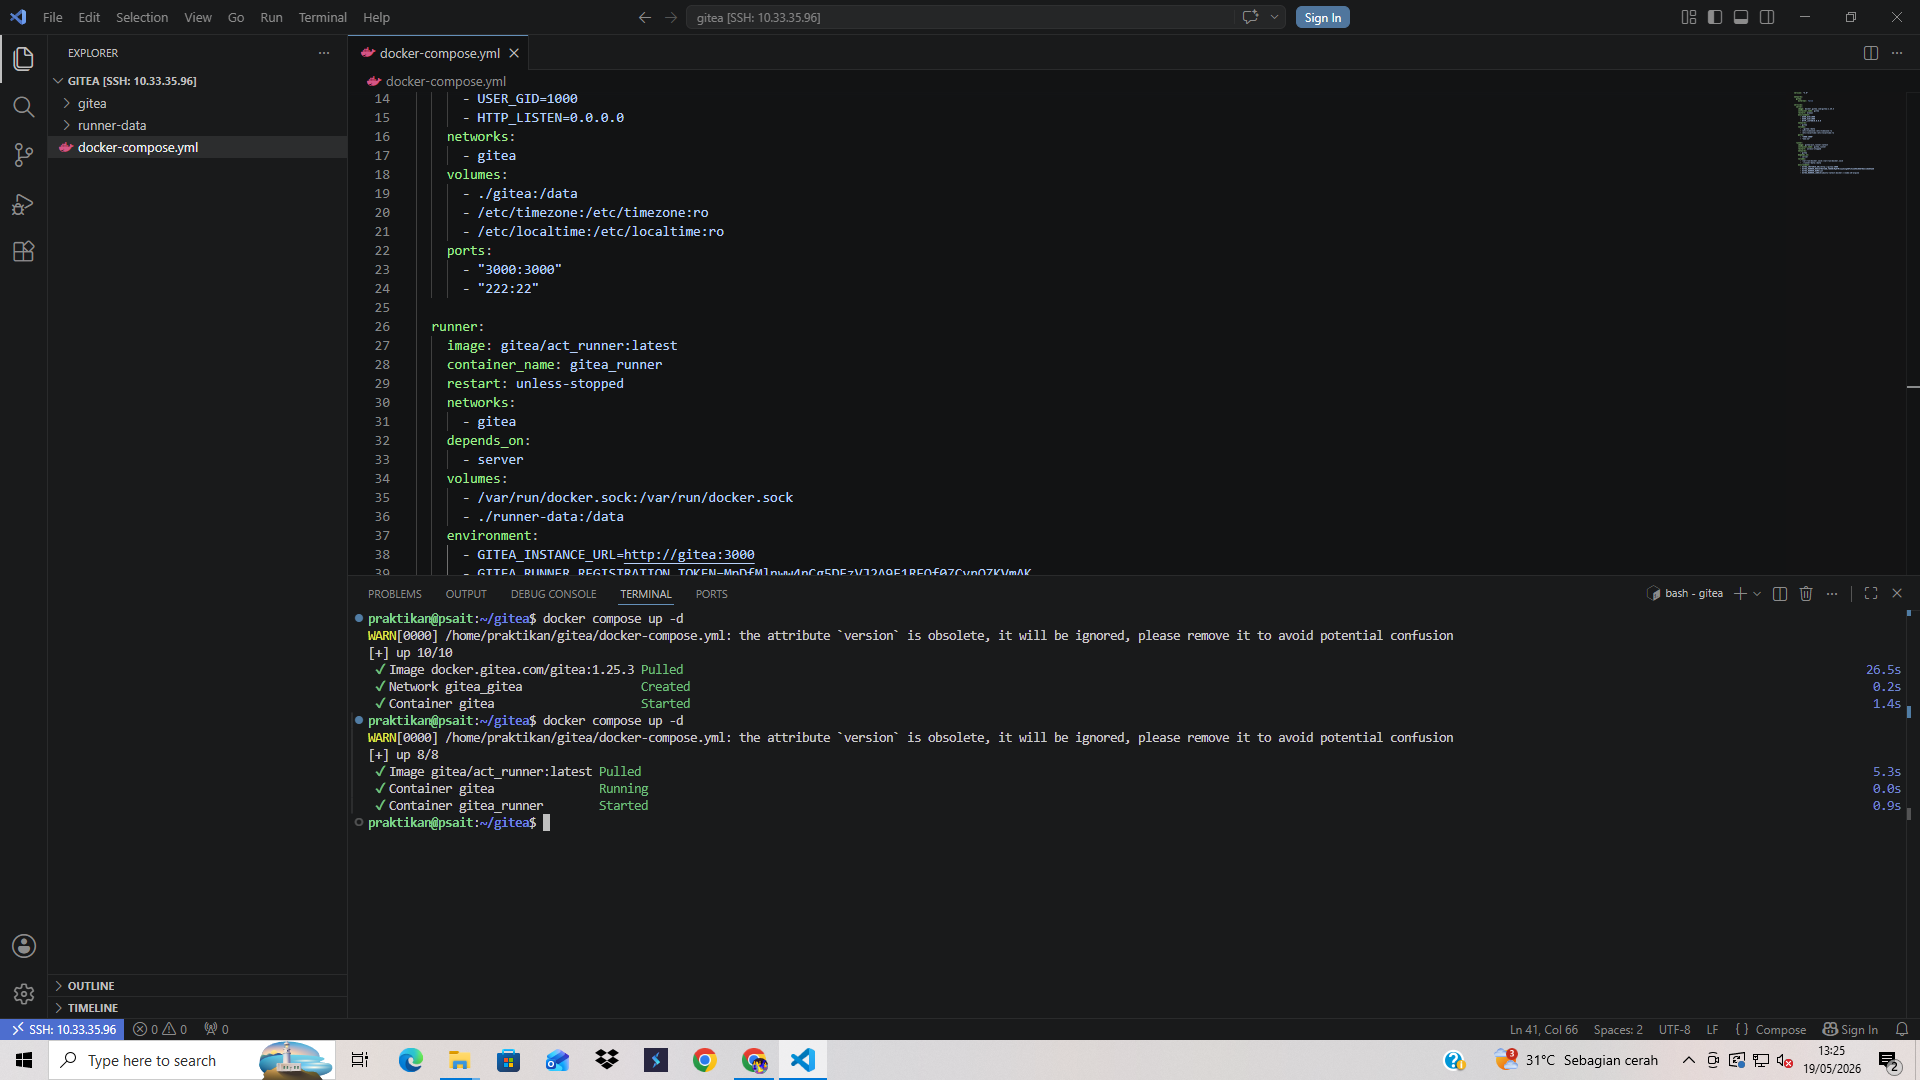
\includegraphics[width=0.95\textwidth]{resource/dokumentasi/13 - jalankan docker compose lagi.png}
  \caption{Menjalankan ulang Docker Compose untuk mengaktifkan Runner}
  \label{fig:p11-13-runner-up}
\end{figure}

\begin{figure}[H]
  \centering
  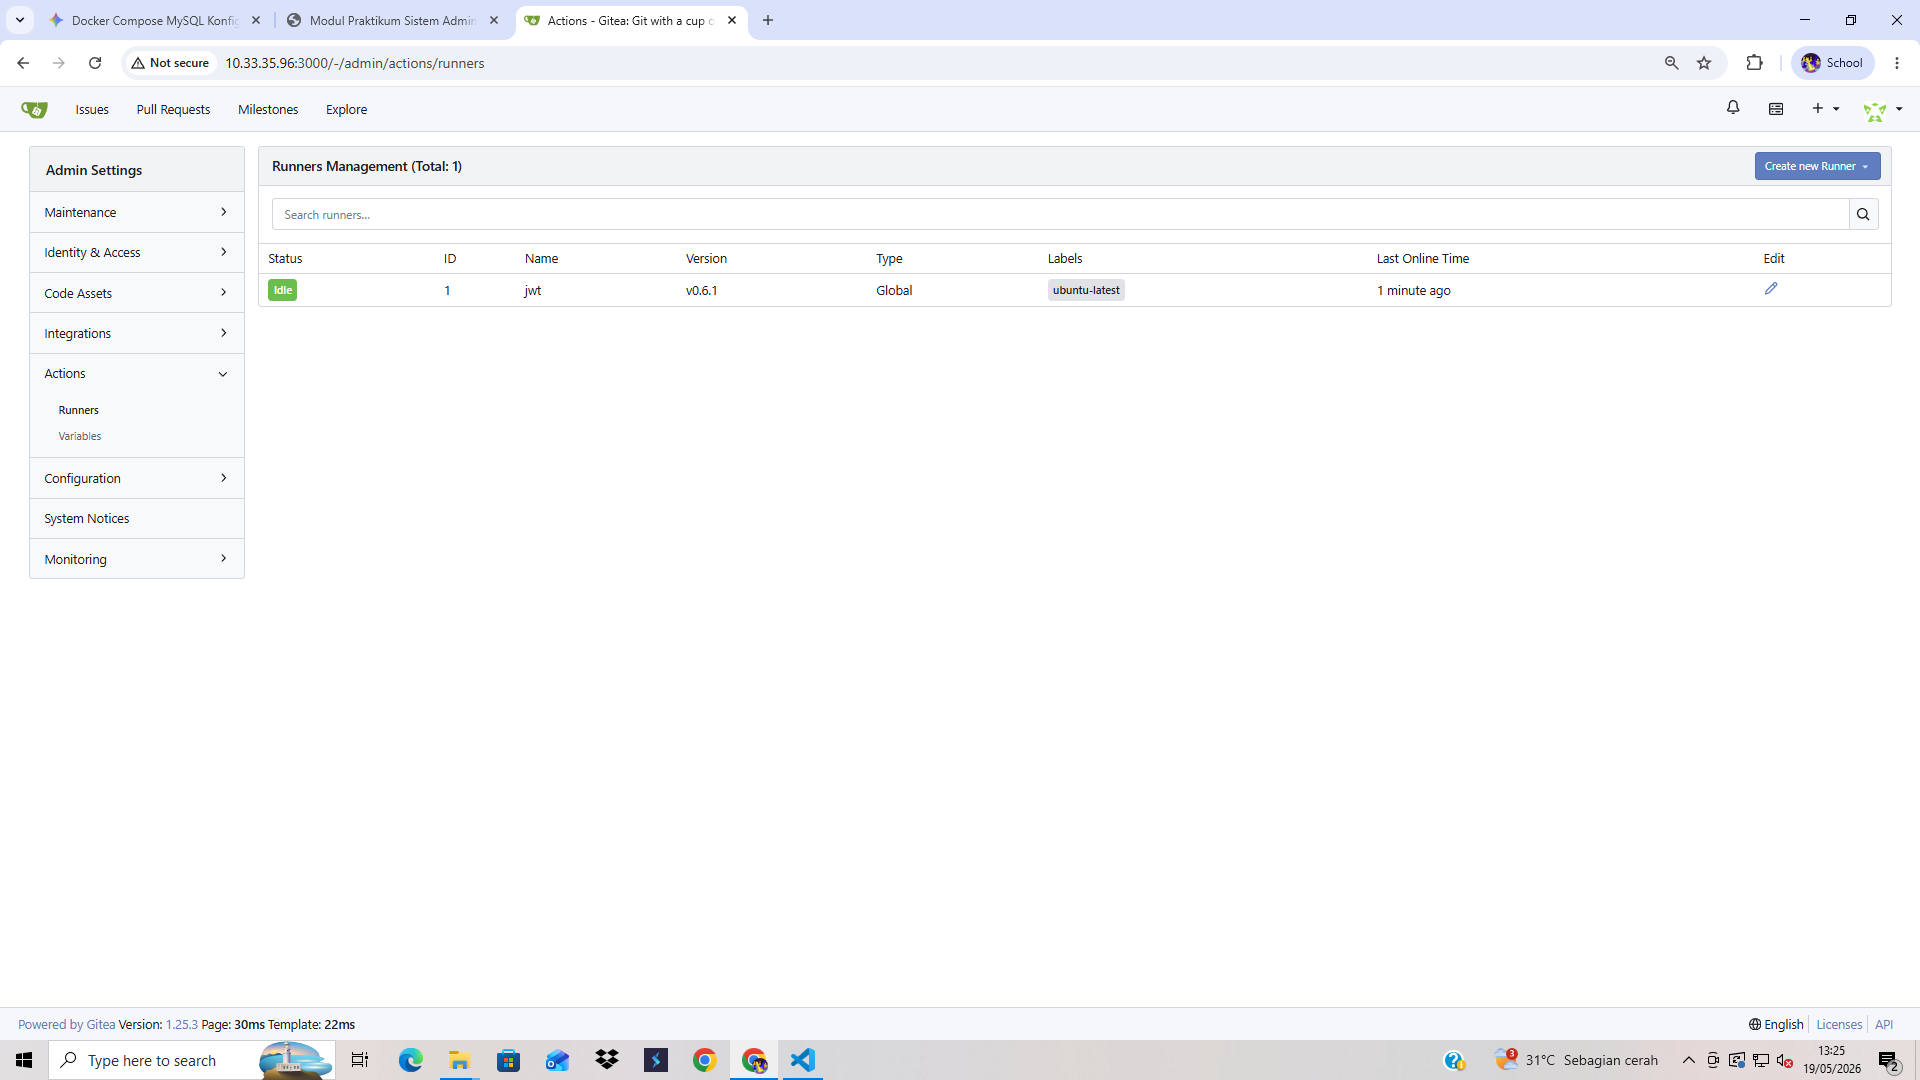
\includegraphics[width=0.95\textwidth]{resource/dokumentasi/14 - hasilnya di gitea.png}
  \caption{Status Runner yang telah berhasil \textit{online} di Gitea}
  \label{fig:p11-14-runner-online}
\end{figure}

\par Langkah berikutnya adalah membuat repositori Git baru di Gitea untuk menampung seluruh berkas source code aplikasi (Gambar \ref{fig:p11-15-new-repo} dan Gambar \ref{fig:p11-16-fill-repo}). Repositori ini dibuat dengan nama \texttt{JWT} menggunakan default branch bernama \texttt{main}. Ketika pembuatan repositori selesai dilakukan (Gambar \ref{fig:p11-17-repo-created}), halaman panduan cepat (\textit{Quick Guide}) akan menyajikan URL remote repository untuk proses deployment awal.

\begin{figure}[H]
  \centering
  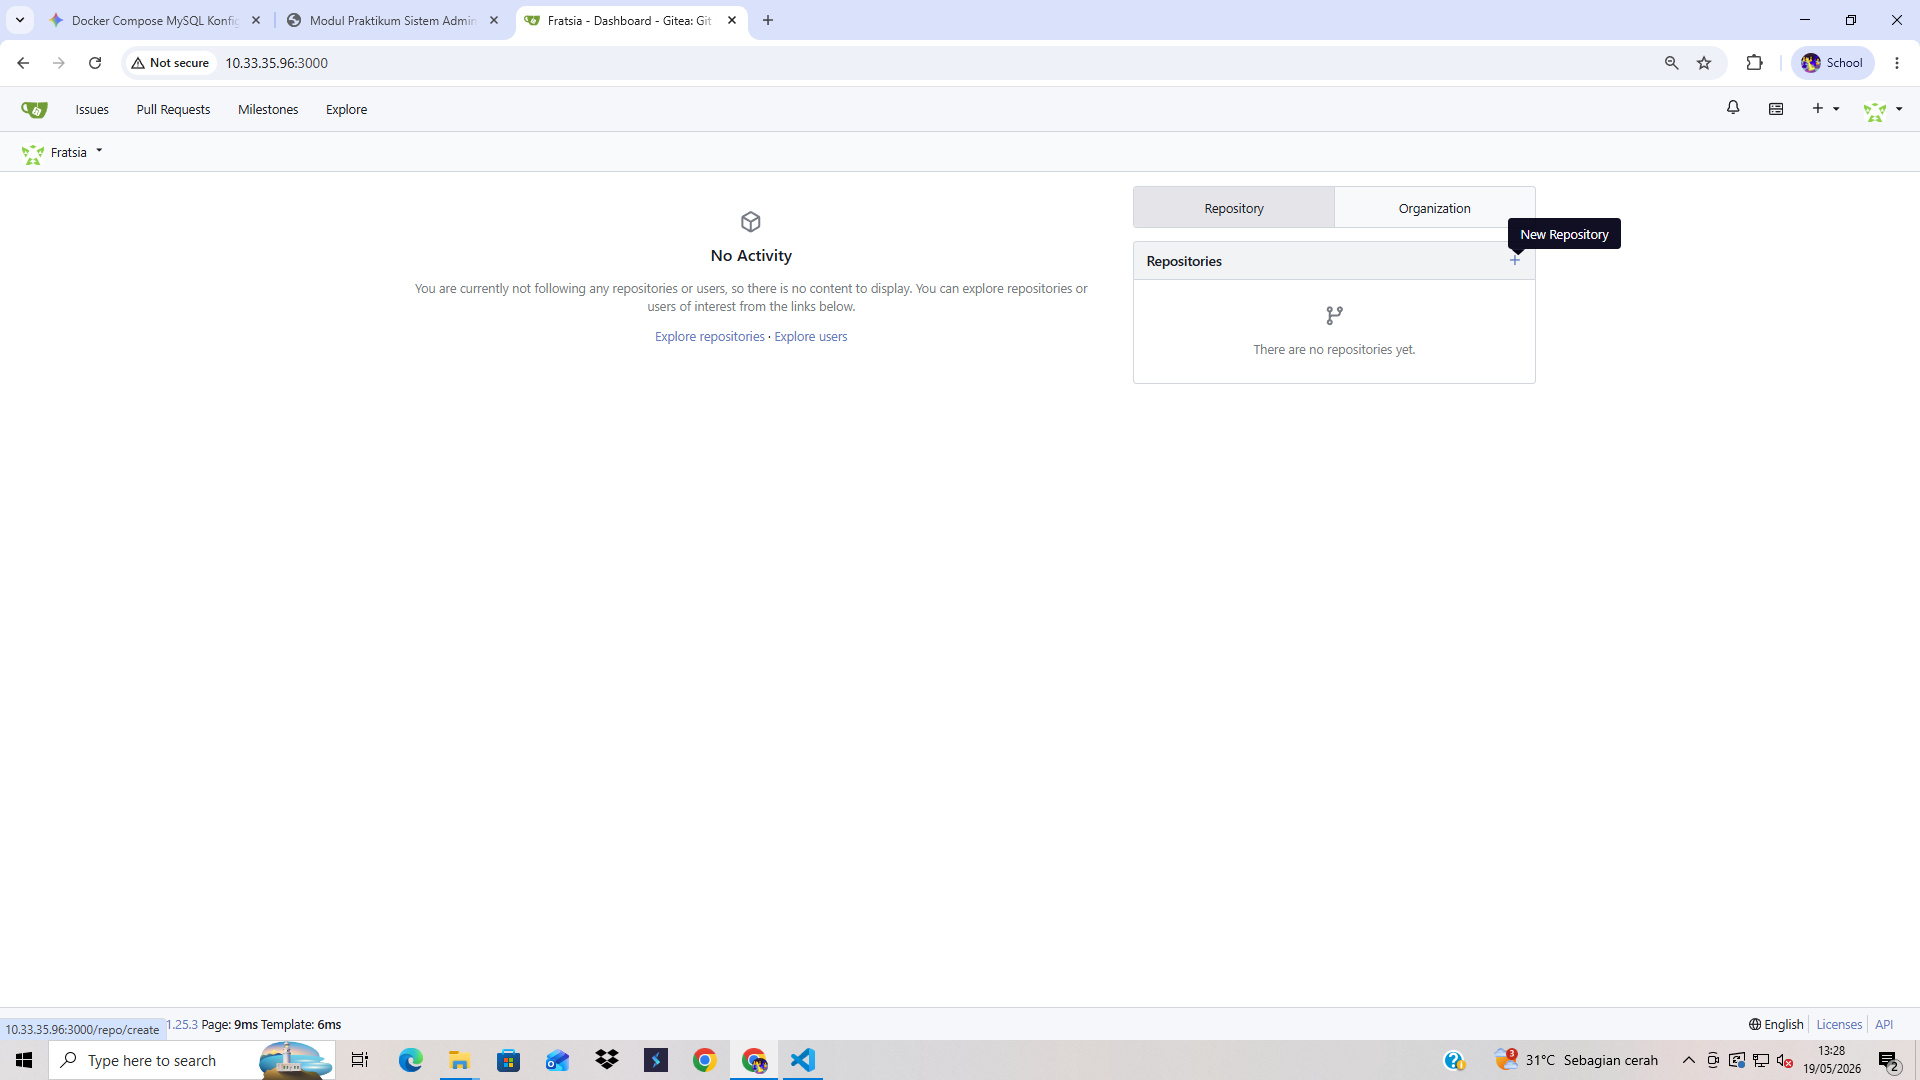
\includegraphics[width=0.95\textwidth]{resource/dokumentasi/15 - klik new repositori.png}
  \caption{Membuat repositori baru melalui antarmuka Gitea}
  \label{fig:p11-15-new-repo}
\end{figure}

\begin{figure}[H]
  \centering
  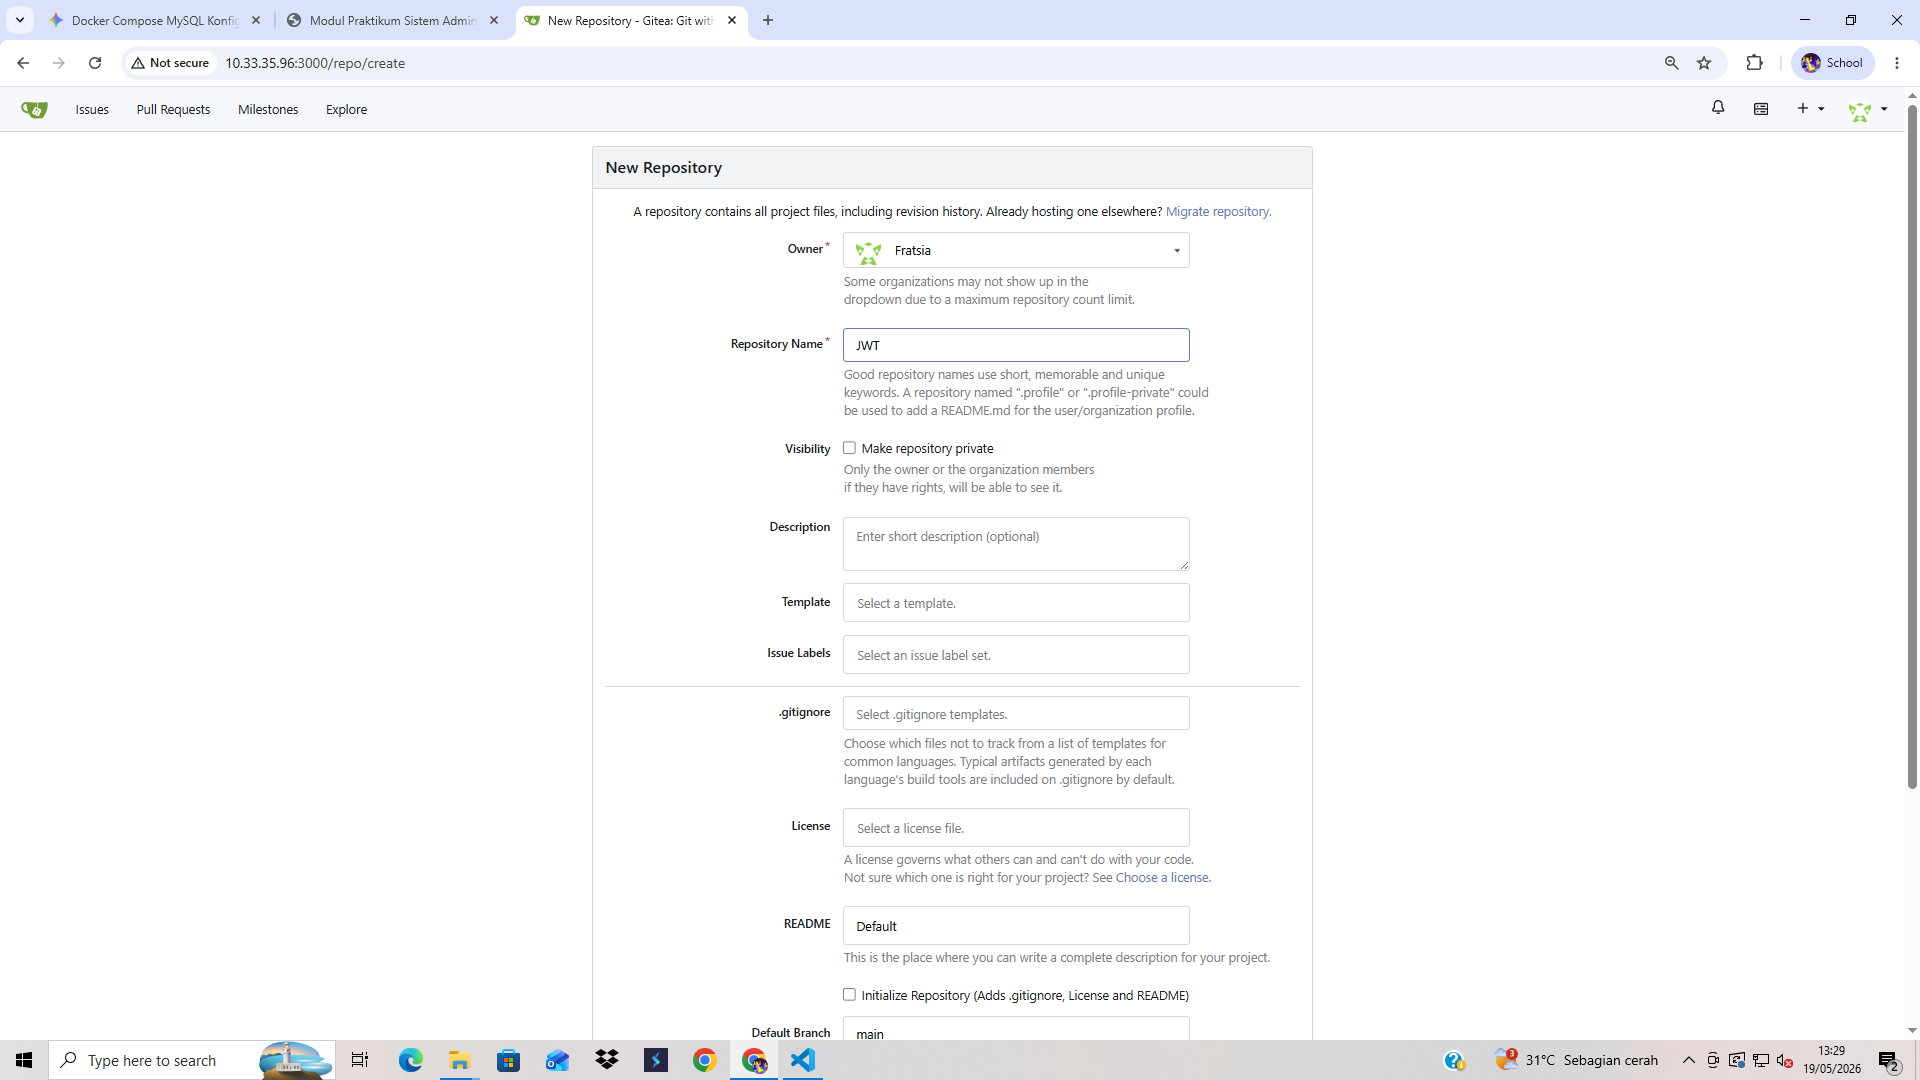
\includegraphics[width=0.95\textwidth]{resource/dokumentasi/16 - pengisian repo baru.png}
  \caption{Mengisi detail repositori baru}
  \label{fig:p11-16-fill-repo}
\end{figure}

\begin{figure}[H]
  \centering
  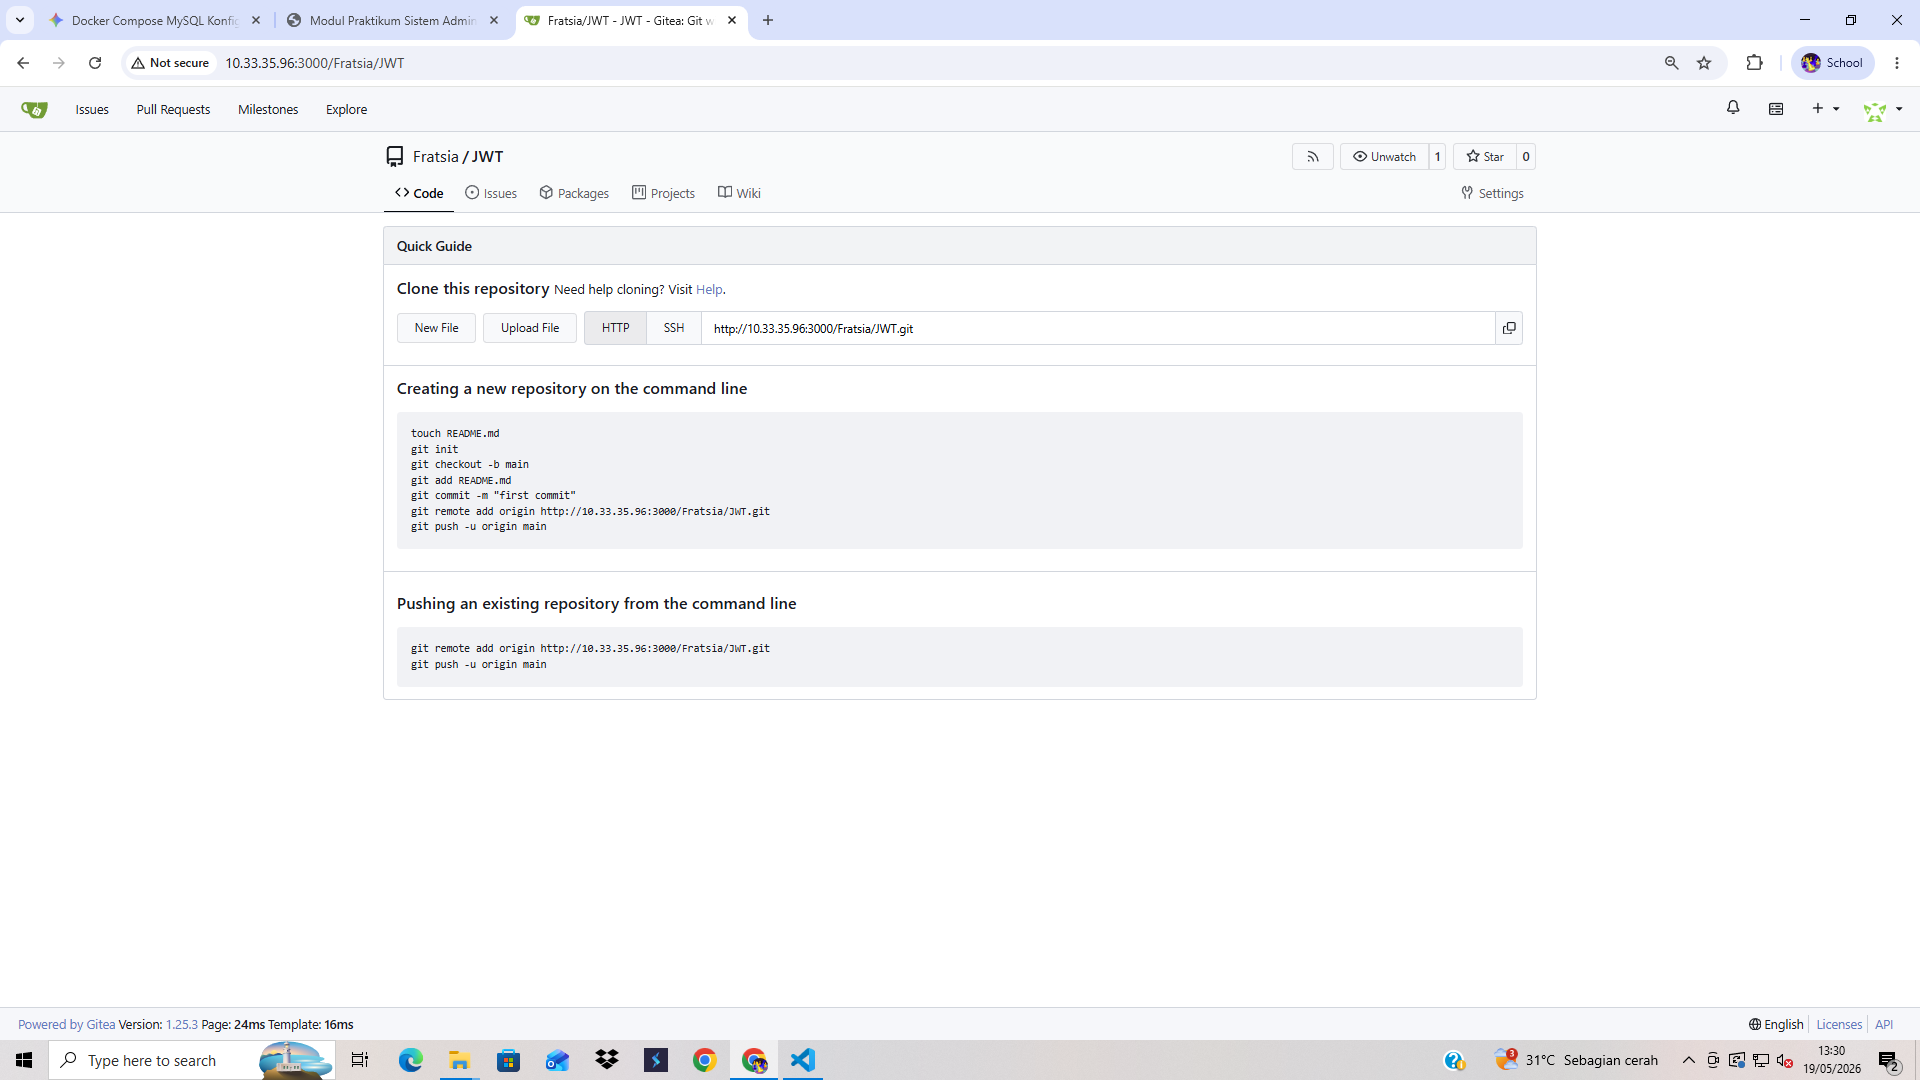
\includegraphics[width=0.95\textwidth]{resource/dokumentasi/17 - Hasil create.png}
  \caption{Repositori aplikasi kosong yang berhasil dibuat}
  \label{fig:p11-17-repo-created}
\end{figure}

\begin{figure}[H]
  \centering
  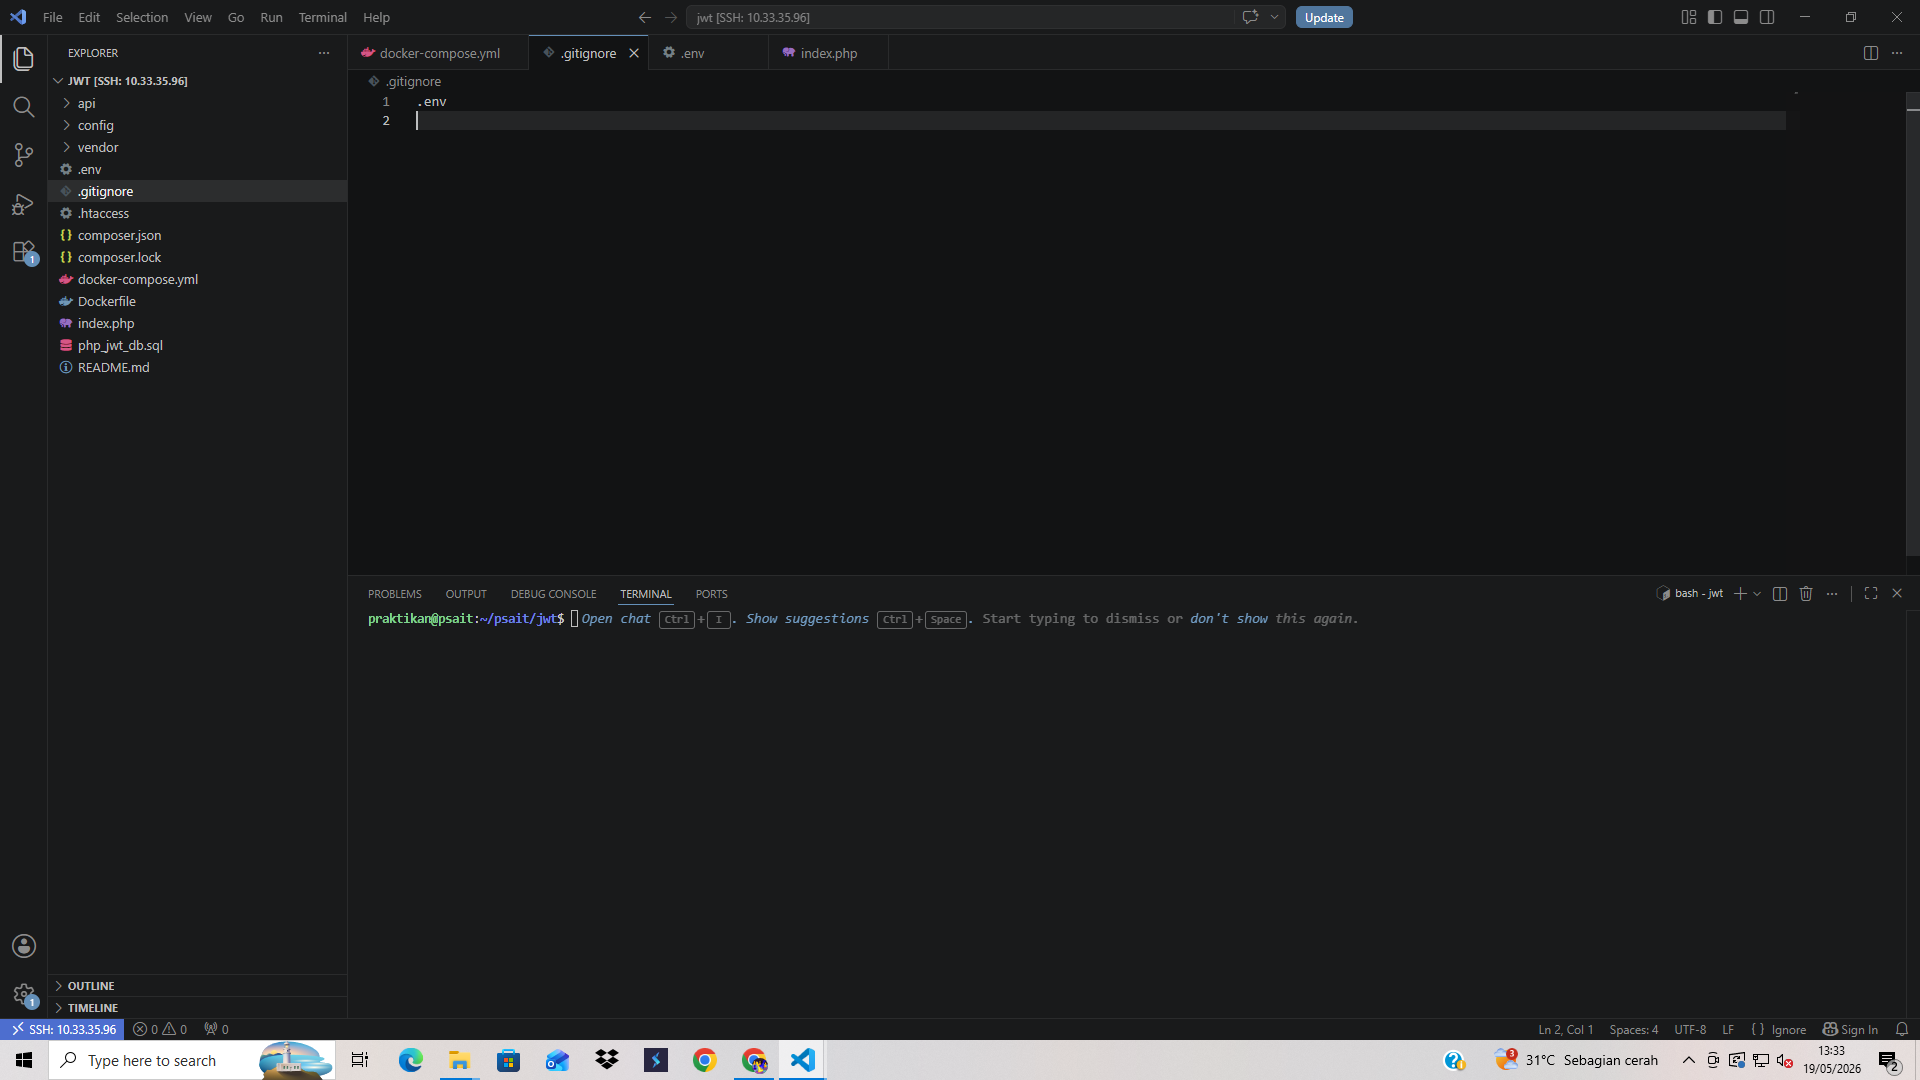
\includegraphics[width=0.95\textwidth]{resource/dokumentasi/18 - tambahkan gitignore.png}
  \caption{Menambahkan file \texttt{.gitignore} untuk mengamankan file \texttt{.env}}
  \label{fig:p11-18-gitignore}
\end{figure}

\par Agar informasi kredensial yang sensitif pada file \texttt{.env} tidak terunggah ke repositori publik, saya mendaftarkan nama file tersebut ke dalam file pengabaian \texttt{.gitignore} (Gambar \ref{fig:p11-18-gitignore}) dengan format konfigurasi seperti pada Listing \ref{lst:p11-gitignore-env}.

\begin{lstlisting}[caption={Isi \texttt{.gitignore} untuk mengabaikan file \texttt{.env}}, label={lst:p11-gitignore-env}]
.env
\end{lstlisting}

\par Proses pengunggahan kode aplikasi ke Gitea dilakukan dengan melakukan inisialisasi git local, menambahkan berkas ke area \textit{staging}, melakukan \textit{commit}, mendaftarkan remote server Gitea, dan menjalankan perintah \texttt{git push} (Gambar \ref{fig:p11-19-push}). Rincian langkah-langkah Git tersebut dirangkum pada Listing \ref{lst:p11-git-push-gitea}. Saat otentikasi push berjalan, akun kredensial administrator Gitea digunakan untuk memberikan izin akses penulisan.

\begin{lstlisting}[caption={Perintah Git untuk \textit{commit} dan \textit{push} ke Gitea}, label={lst:p11-git-push-gitea}]
git init
git add .
git commit -m "first commit"
git branch -M main
git remote add origin http://10.33.35.96:3000/Fratsia/JWT.git
git push -u origin main
\end{lstlisting}

\par Setelah proses push berhasil diselesaikan, struktur direktori beserta berkas source code aplikasi akan langsung tersaji pada antarmuka repositori Gitea (Gambar \ref{fig:p11-20-push-result}).

\begin{figure}[H]
  \centering
  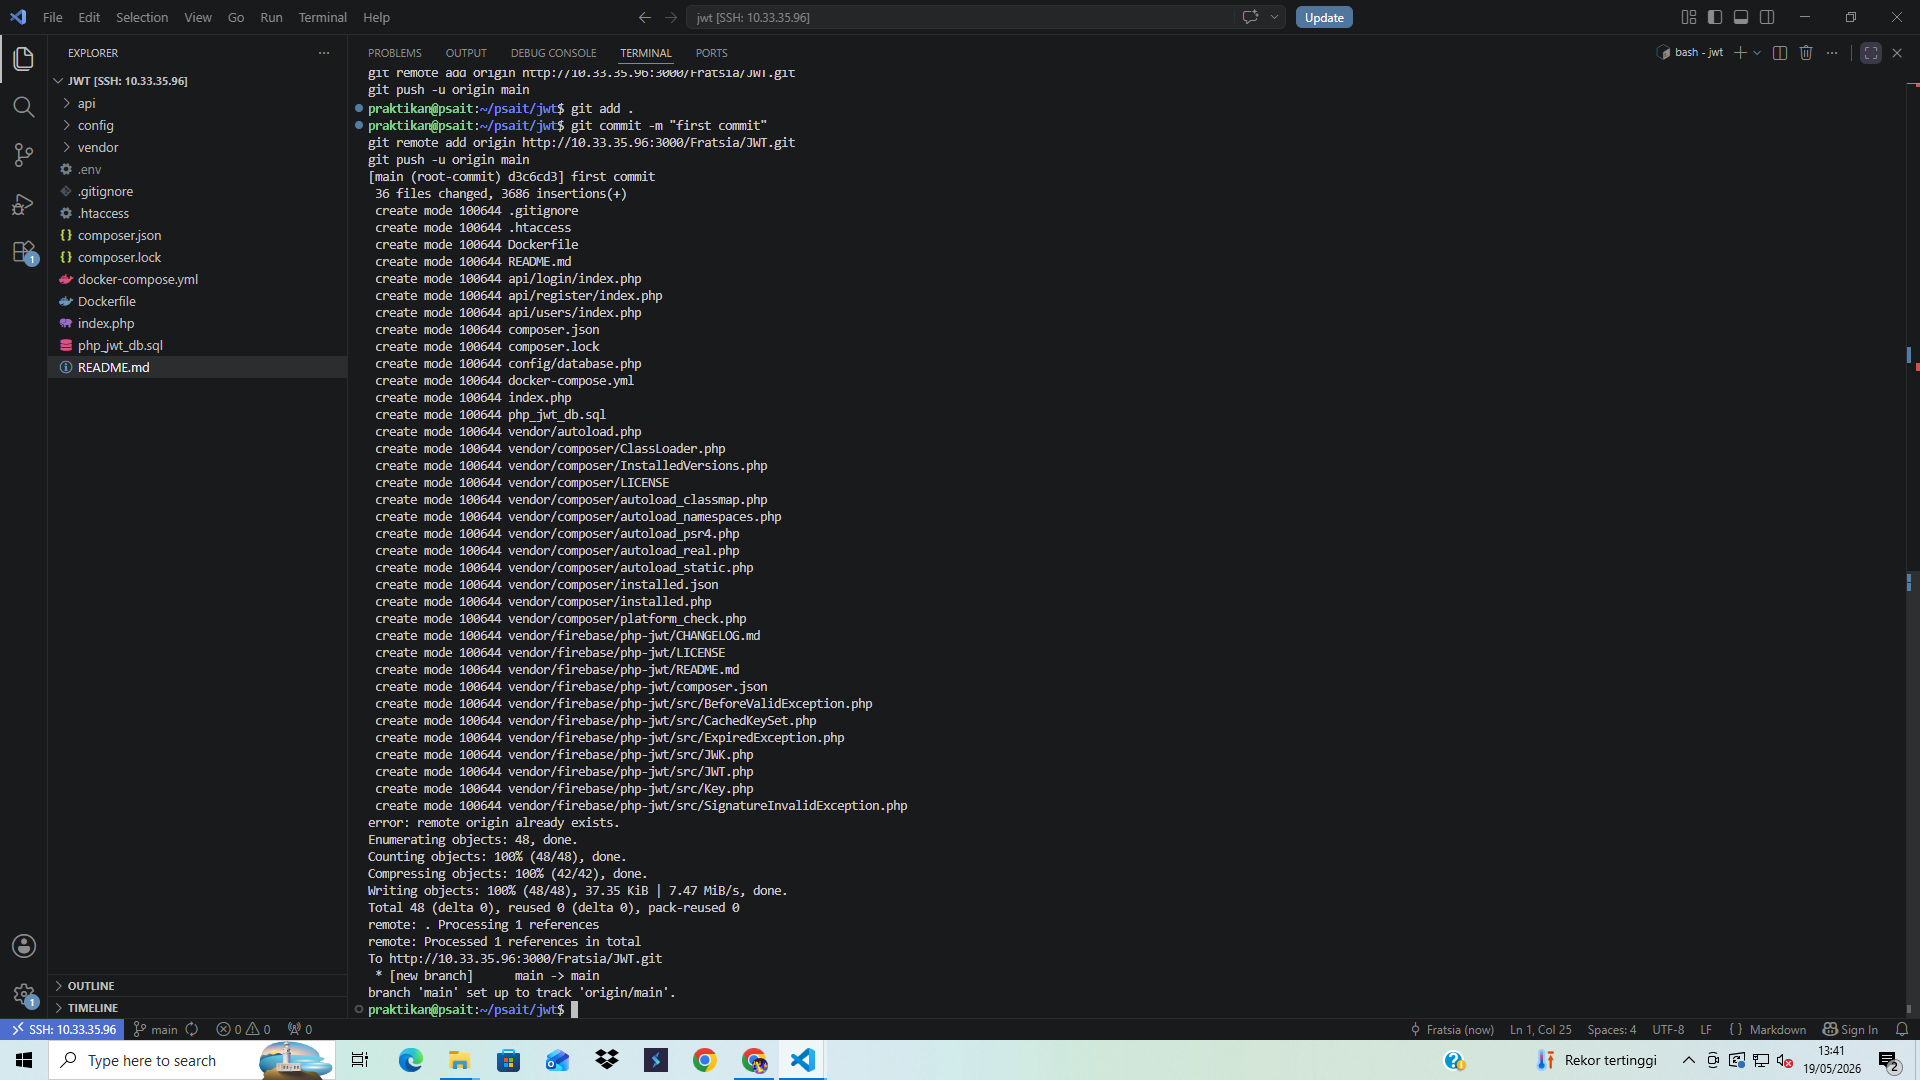
\includegraphics[width=0.95\textwidth]{resource/dokumentasi/19 - Push ke gitea.png}
  \caption{Melakukan push source code lokal ke Gitea}
  \label{fig:p11-19-push}
\end{figure}

\begin{figure}[H]
  \centering
  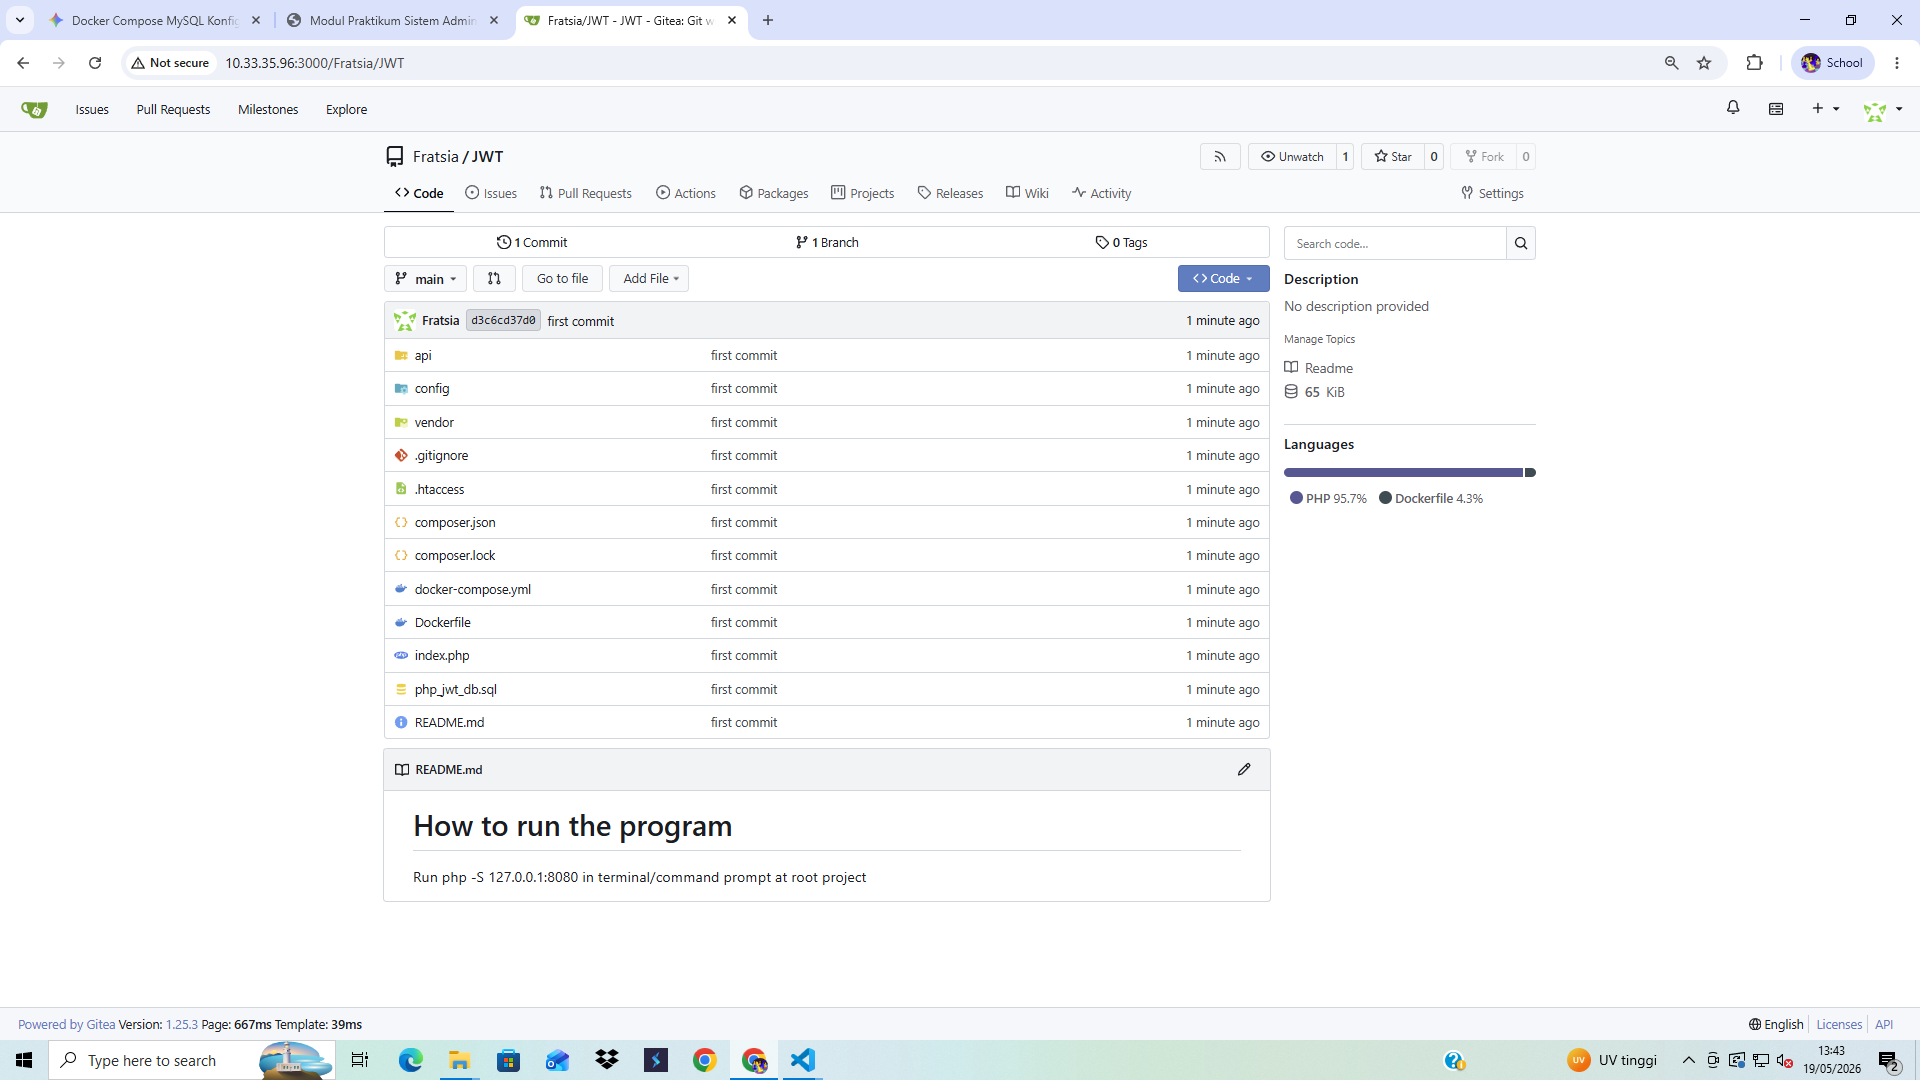
\includegraphics[width=0.95\textwidth]{resource/dokumentasi/20 - hasil gitea.png}
  \caption{Hasil source code yang berhasil terunggah ke Gitea}
  \label{fig:p11-20-push-result}
\end{figure}

\subsection{Clone repository jwt di local pc}

\par Setelah repositori berhasil dibuat pada platform Gitea di VPS, langkah berikutnya adalah menduplikasi (kloning) kode sumber tersebut ke komputer lokal agar proses pengembangan berkas dapat dilakukan. Proses ini dilakukan dengan menyalin URL repositori yang tersedia di Gitea (Gambar \ref{fig:p11-21-clone}).

\begin{figure}[H]
  \centering
  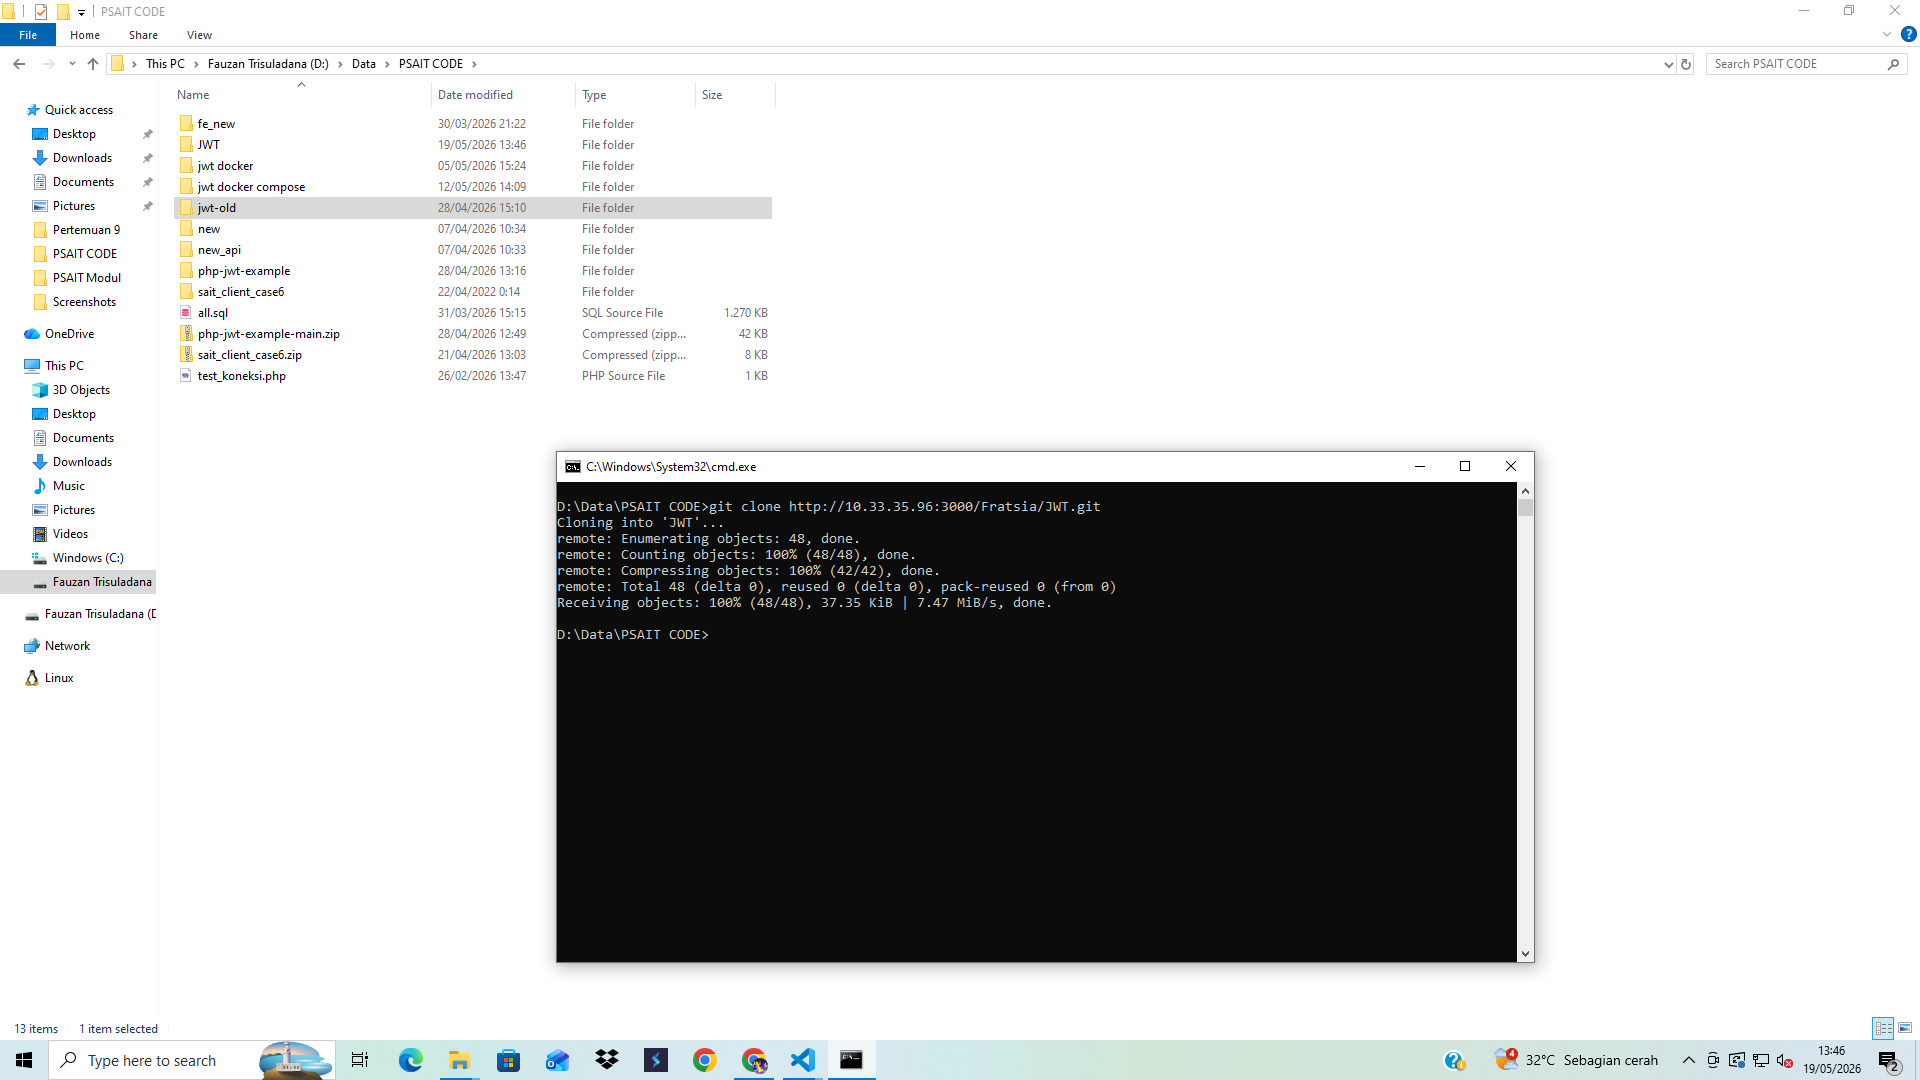
\includegraphics[width=0.95\textwidth]{resource/dokumentasi/21 - clone di local.png}
  \caption{Melakukan kloning repositori ke komputer lokal}
  \label{fig:p11-21-clone}
\end{figure}

\par Selanjutnya, terminal pada komputer lokal dijalankan dan perintah \texttt{git clone} dieksekusi menggunakan URL repositori tersebut. Setelah proses kloning selesai, direktori proyek dibuka menggunakan editor Visual Studio Code untuk mempermudah modifikasi kode (Gambar \ref{fig:p11-22-vscode}). Berkas konfigurasi sensitif seperti \texttt{.env} tidak ikut terunduh karena telah diabaikan menggunakan berkas \texttt{.gitignore} pada tahap sebelumnya.

\begin{figure}[H]
  \centering
  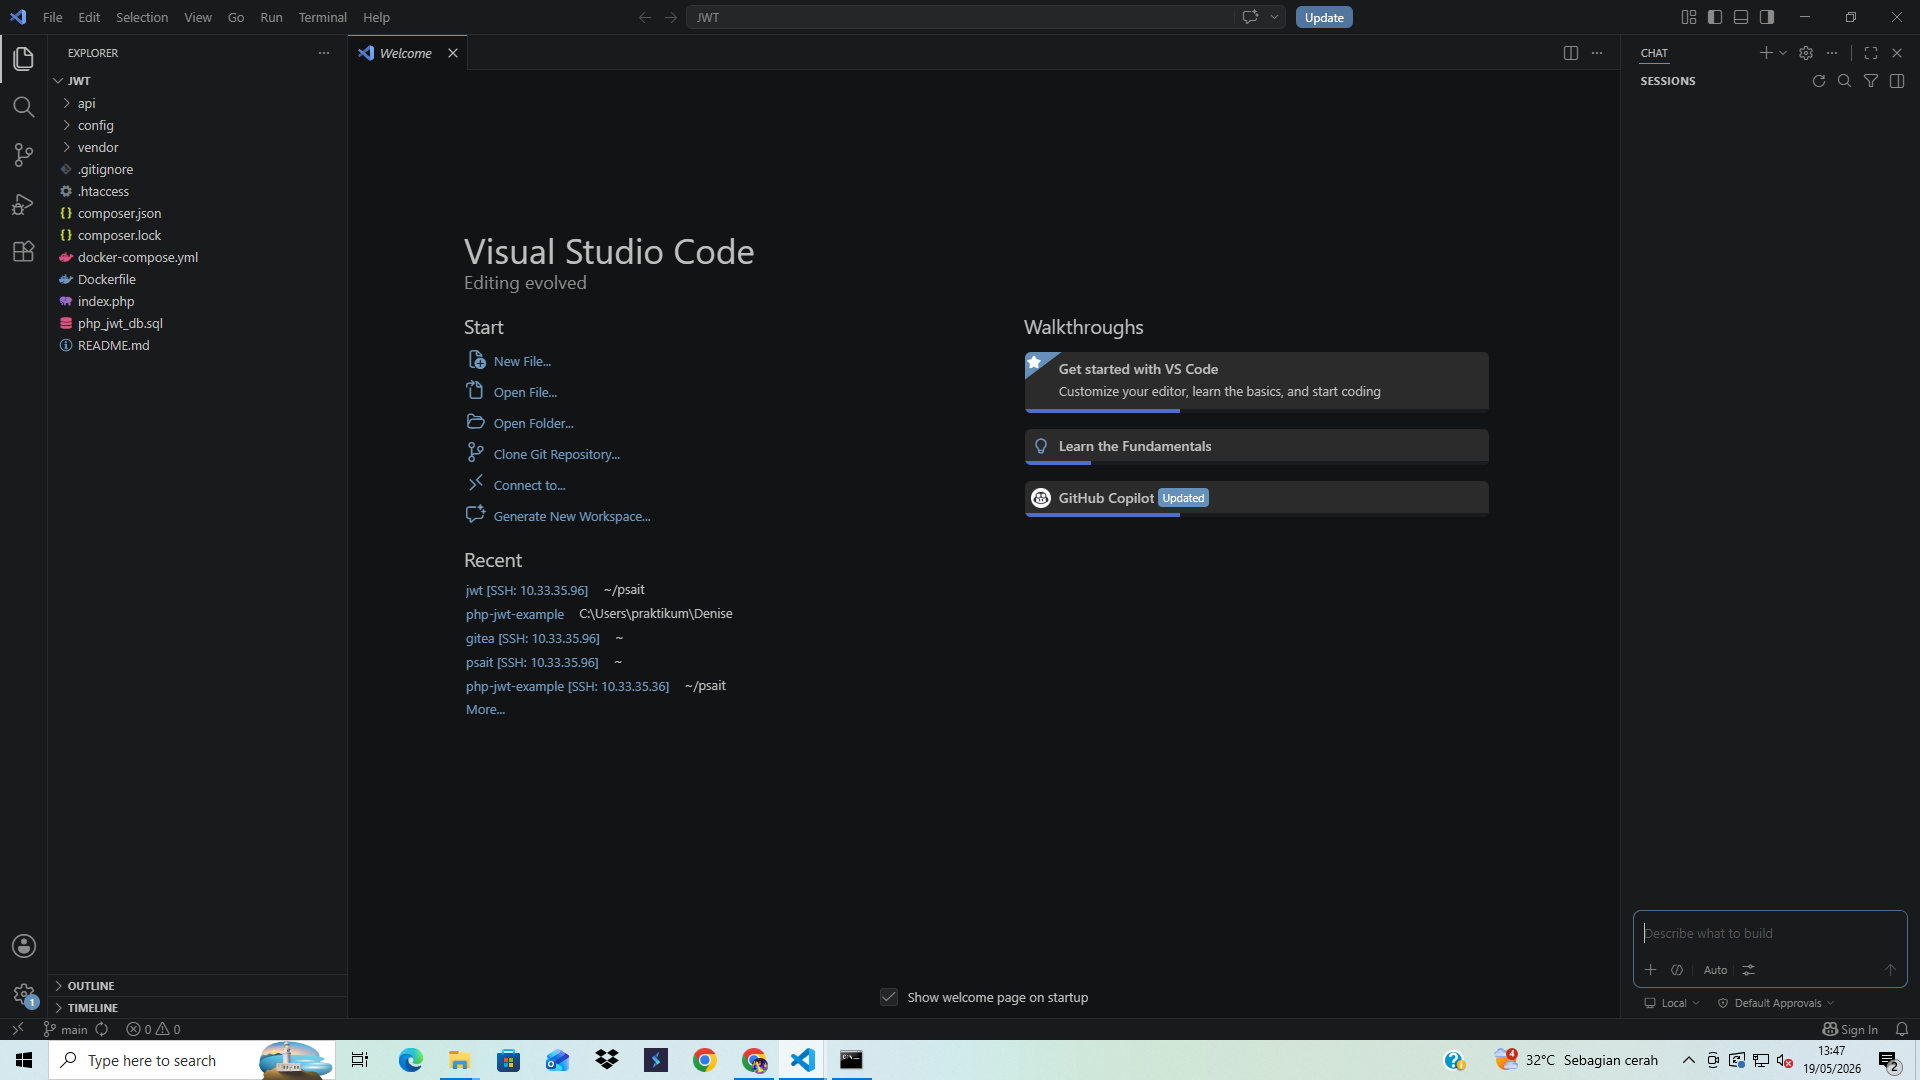
\includegraphics[width=0.95\textwidth]{resource/dokumentasi/22- buka folder hasil clone di vscode.png}
  \caption{Membuka hasil \textit{clone} di VS Code}
  \label{fig:p11-22-vscode}
\end{figure}

\subsection{Implementasi Gitea runner untuk CICD}

\par Agar proses deployment aplikasi pada VPS dapat berjalan secara otomatis, saya mengimplementasikan layanan Gitea Runner. Konfigurasi alur kerja (workflow) CI/CD didefinisikan dengan membuat berkas baru bernama \texttt{deploys.yaml} di dalam direktori khusus \texttt{.gitea/workflows/} pada komputer lokal (Gambar \ref{fig:p11-23-deploys}).

\begin{figure}[H]
  \centering
  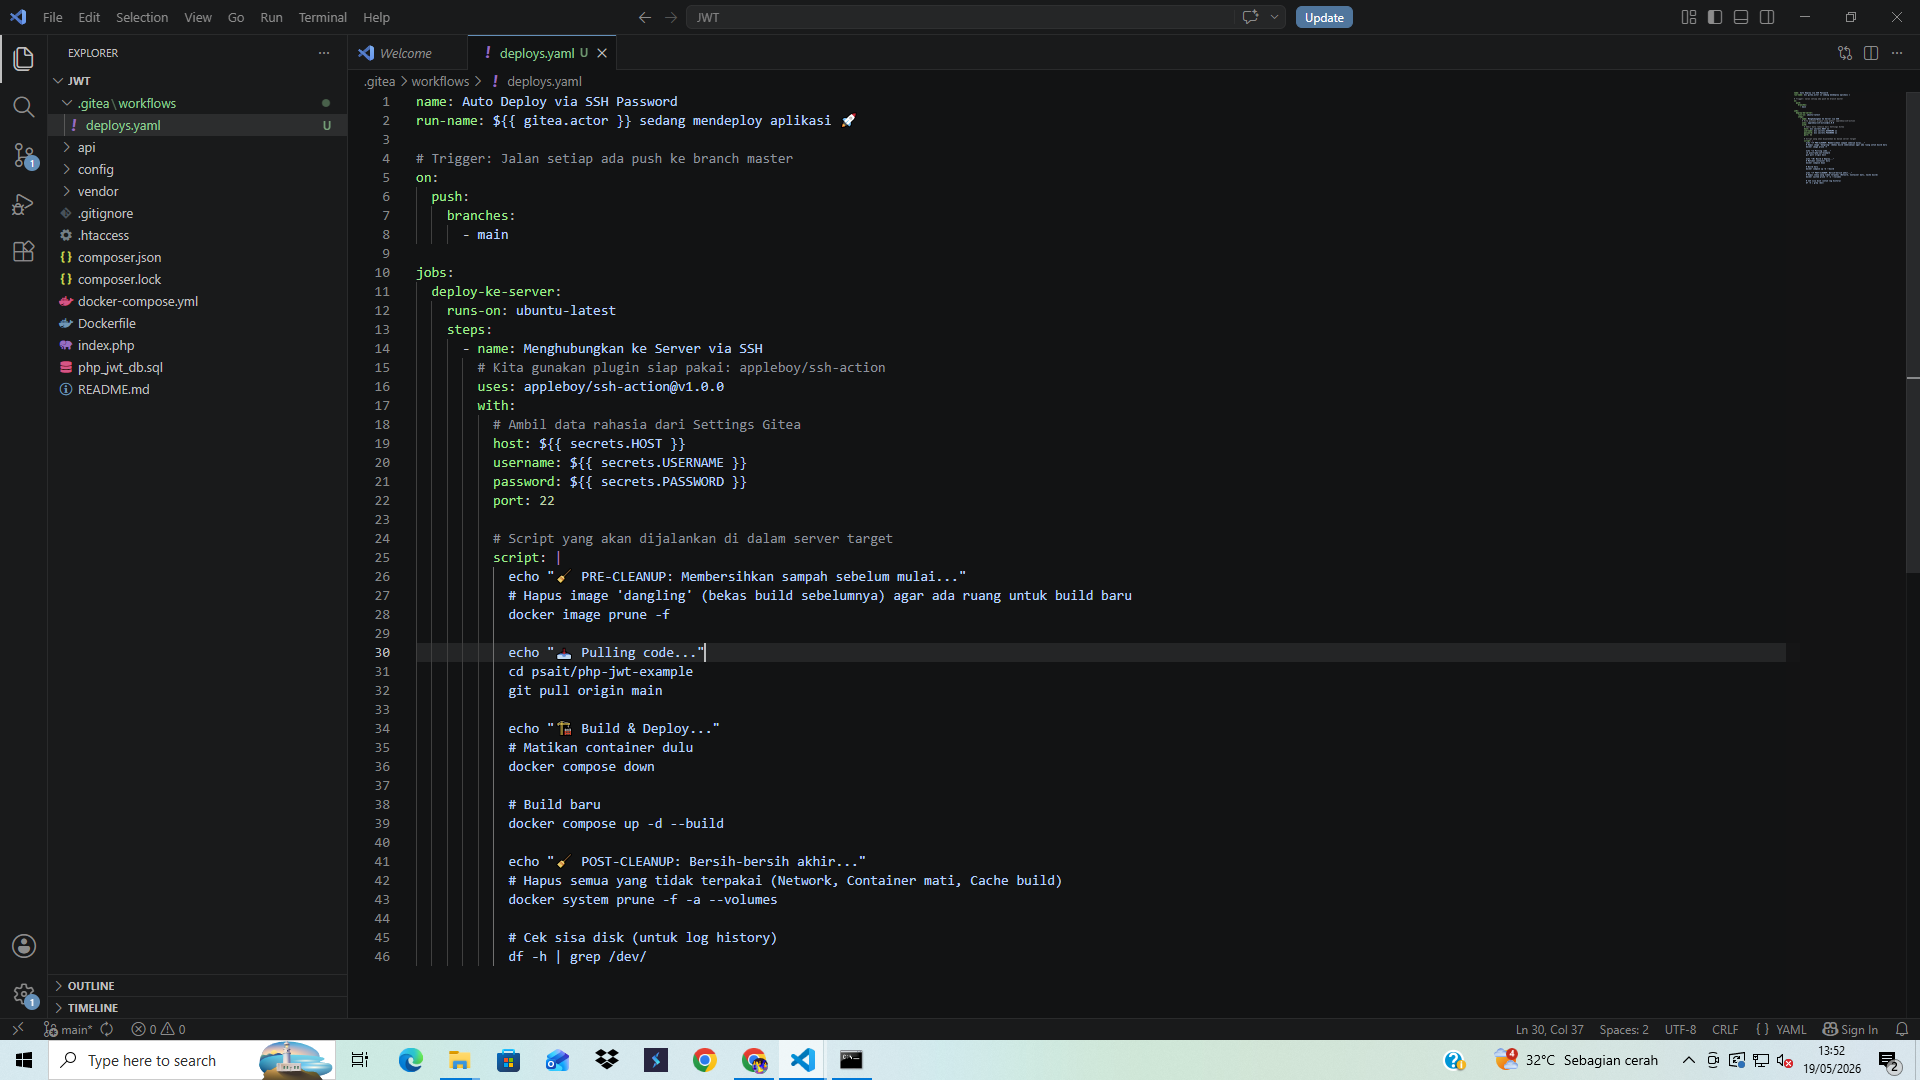
\includegraphics[width=0.95\textwidth]{resource/dokumentasi/23 - tambahkan file deploys.png}
  \caption{Membuat file \textit{workflow} \texttt{deploys.yaml} untuk otomatisasi CI/CD}
  \label{fig:p11-23-deploys}
\end{figure}

\par Alur kerja pada \texttt{deploys.yaml} diatur agar terpicu secara otomatis setiap ada aktivitas push ke branch \texttt{main}. Tahapan di dalamnya meliputi pembuatan koneksi SSH ke VPS menggunakan aksi pihak ketiga \texttt{appleboy/ssh-action}, yang kemudian mengeksekusi perintah untuk menarik kode terbaru (\texttt{git pull}), menghentikan container Docker yang sedang berjalan, membangun kembali image (\texttt{docker compose up -d --build}), dan membersihkan sisa ruang penyimpanan yang tidak terpakai.

\par Guna menjaga keamanan informasi kredensial yang sensitif seperti alamat IP, username, dan password SSH server VPS, data tersebut disimpan menggunakan fitur \textit{Secrets} pada pengaturan repositori Gitea. Saya menambahkan tiga variabel rahasia baru, yaitu \texttt{HOST} untuk alamat IP VPS (Gambar \ref{fig:p11-24-secret-host}), \texttt{USERNAME} untuk identitas pengguna SSH VPS (Gambar \ref{fig:p11-25-secret-user}), dan \texttt{PASSWORD} untuk kunci autentikasi masuk (Gambar \ref{fig:p11-26-secret-pass}).

\begin{figure}[H]
  \centering
  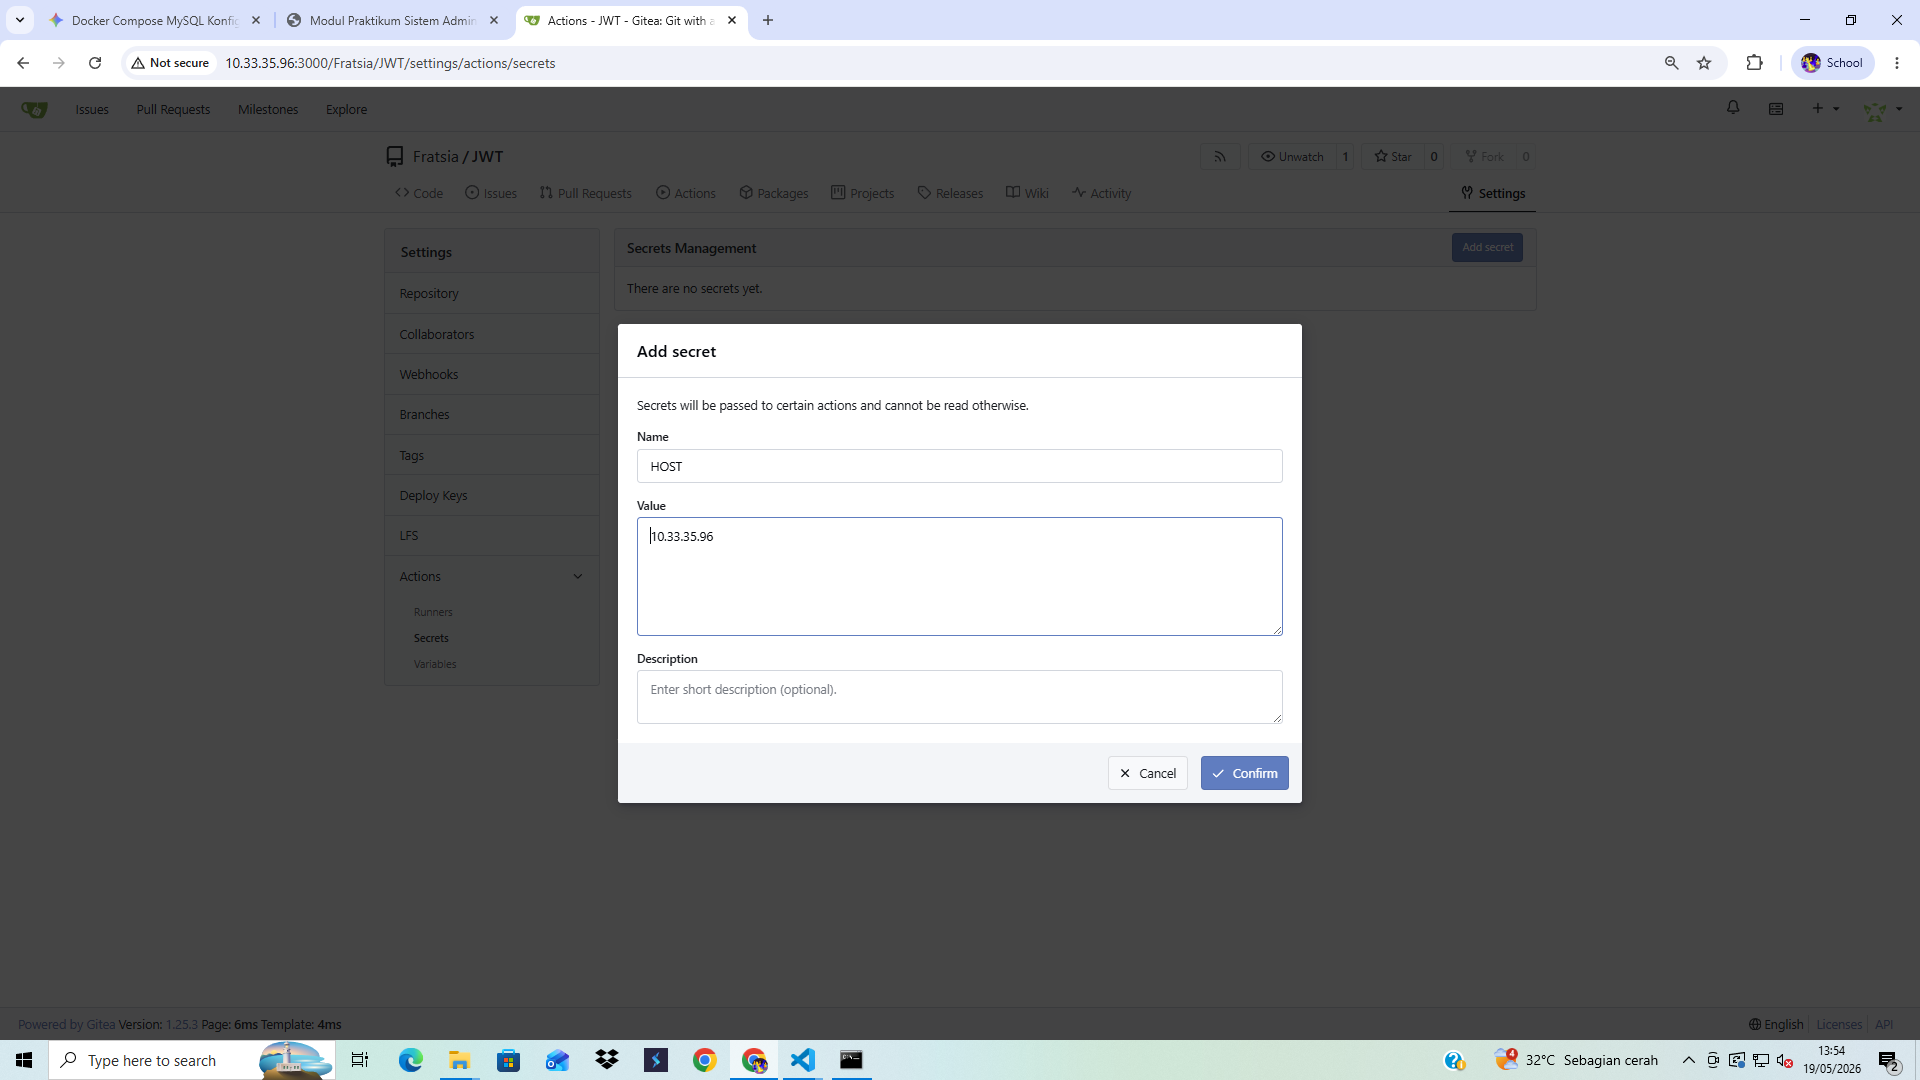
\includegraphics[width=0.95\textwidth]{resource/dokumentasi/24 - tambahkan secret host.png}
  \caption{Menambahkan Secret untuk \texttt{HOST} SSH}
  \label{fig:p11-24-secret-host}
\end{figure}

\begin{figure}[H]
  \centering
  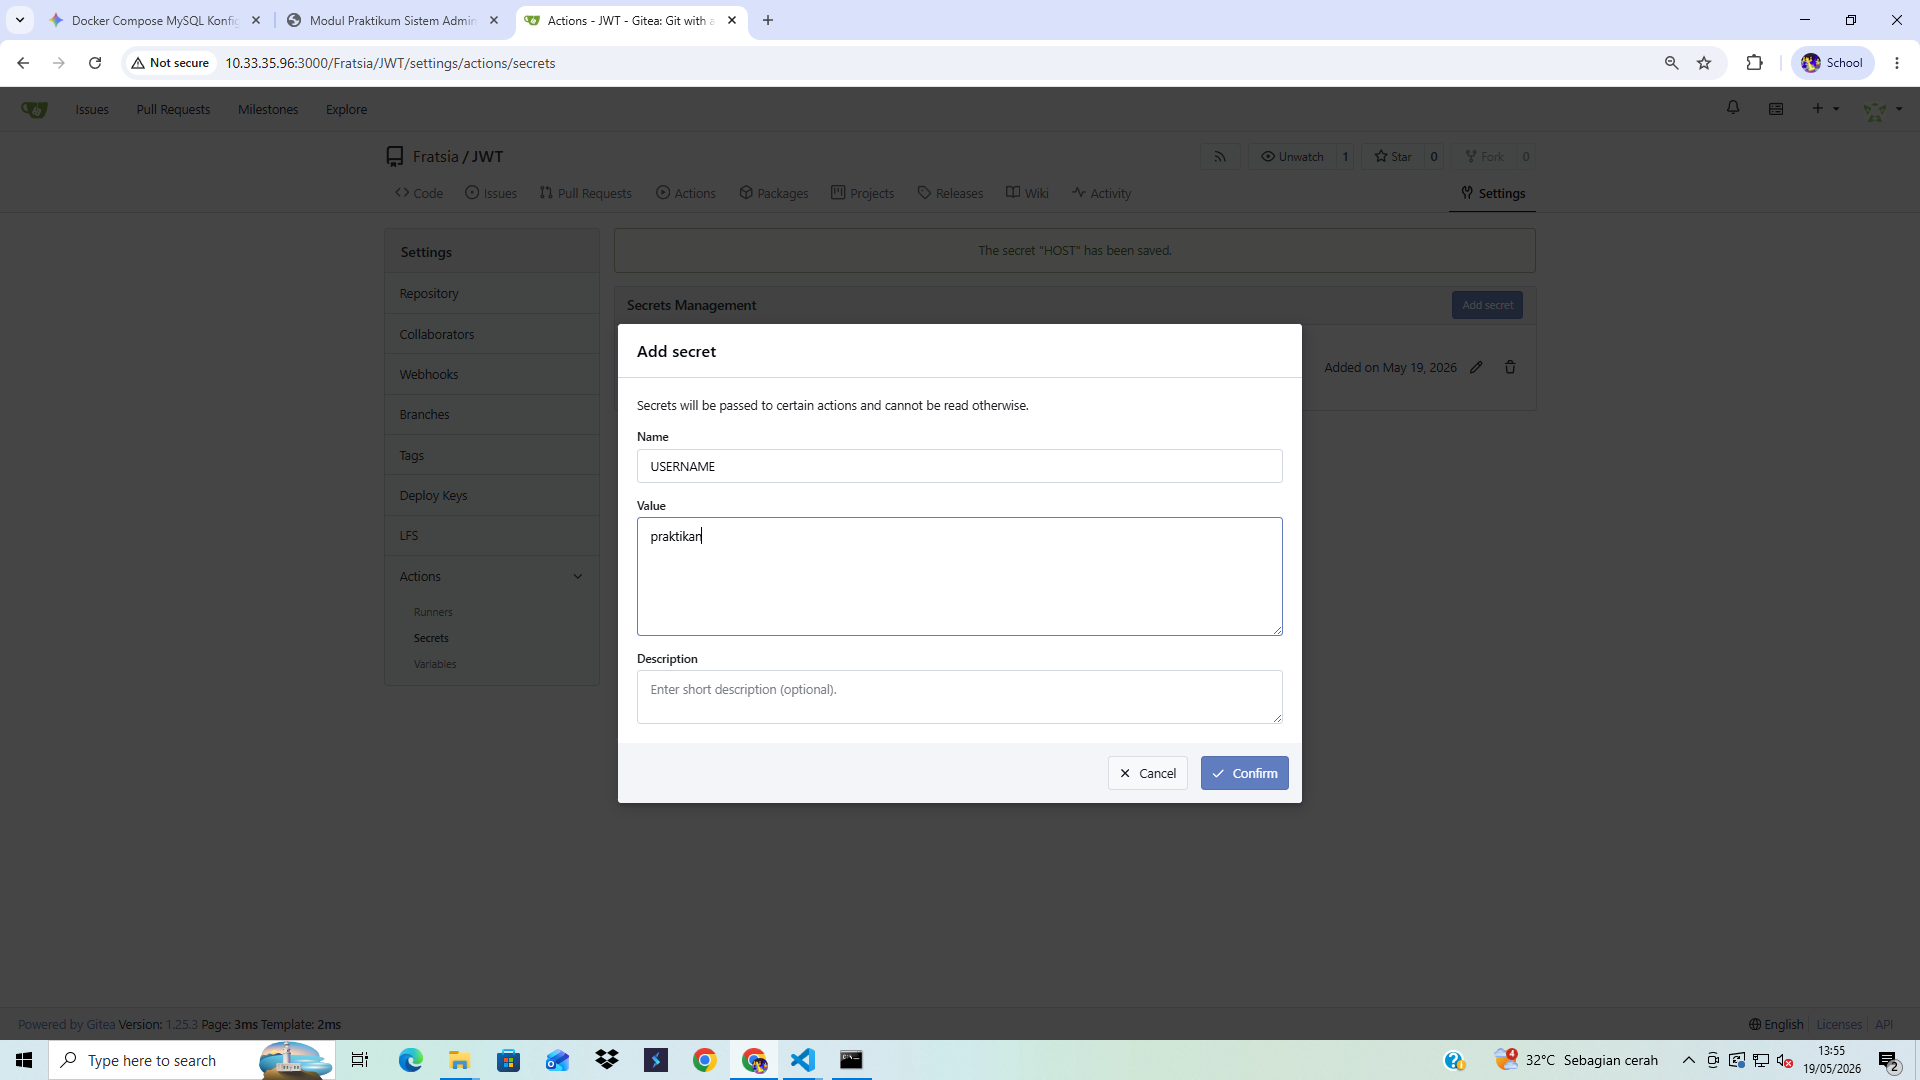
\includegraphics[width=0.95\textwidth]{resource/dokumentasi/25 - tambahkan secret username.png}
  \caption{Menambahkan Secret untuk \texttt{USERNAME} SSH}
  \label{fig:p11-25-secret-user}
\end{figure}

\begin{figure}[H]
  \centering
  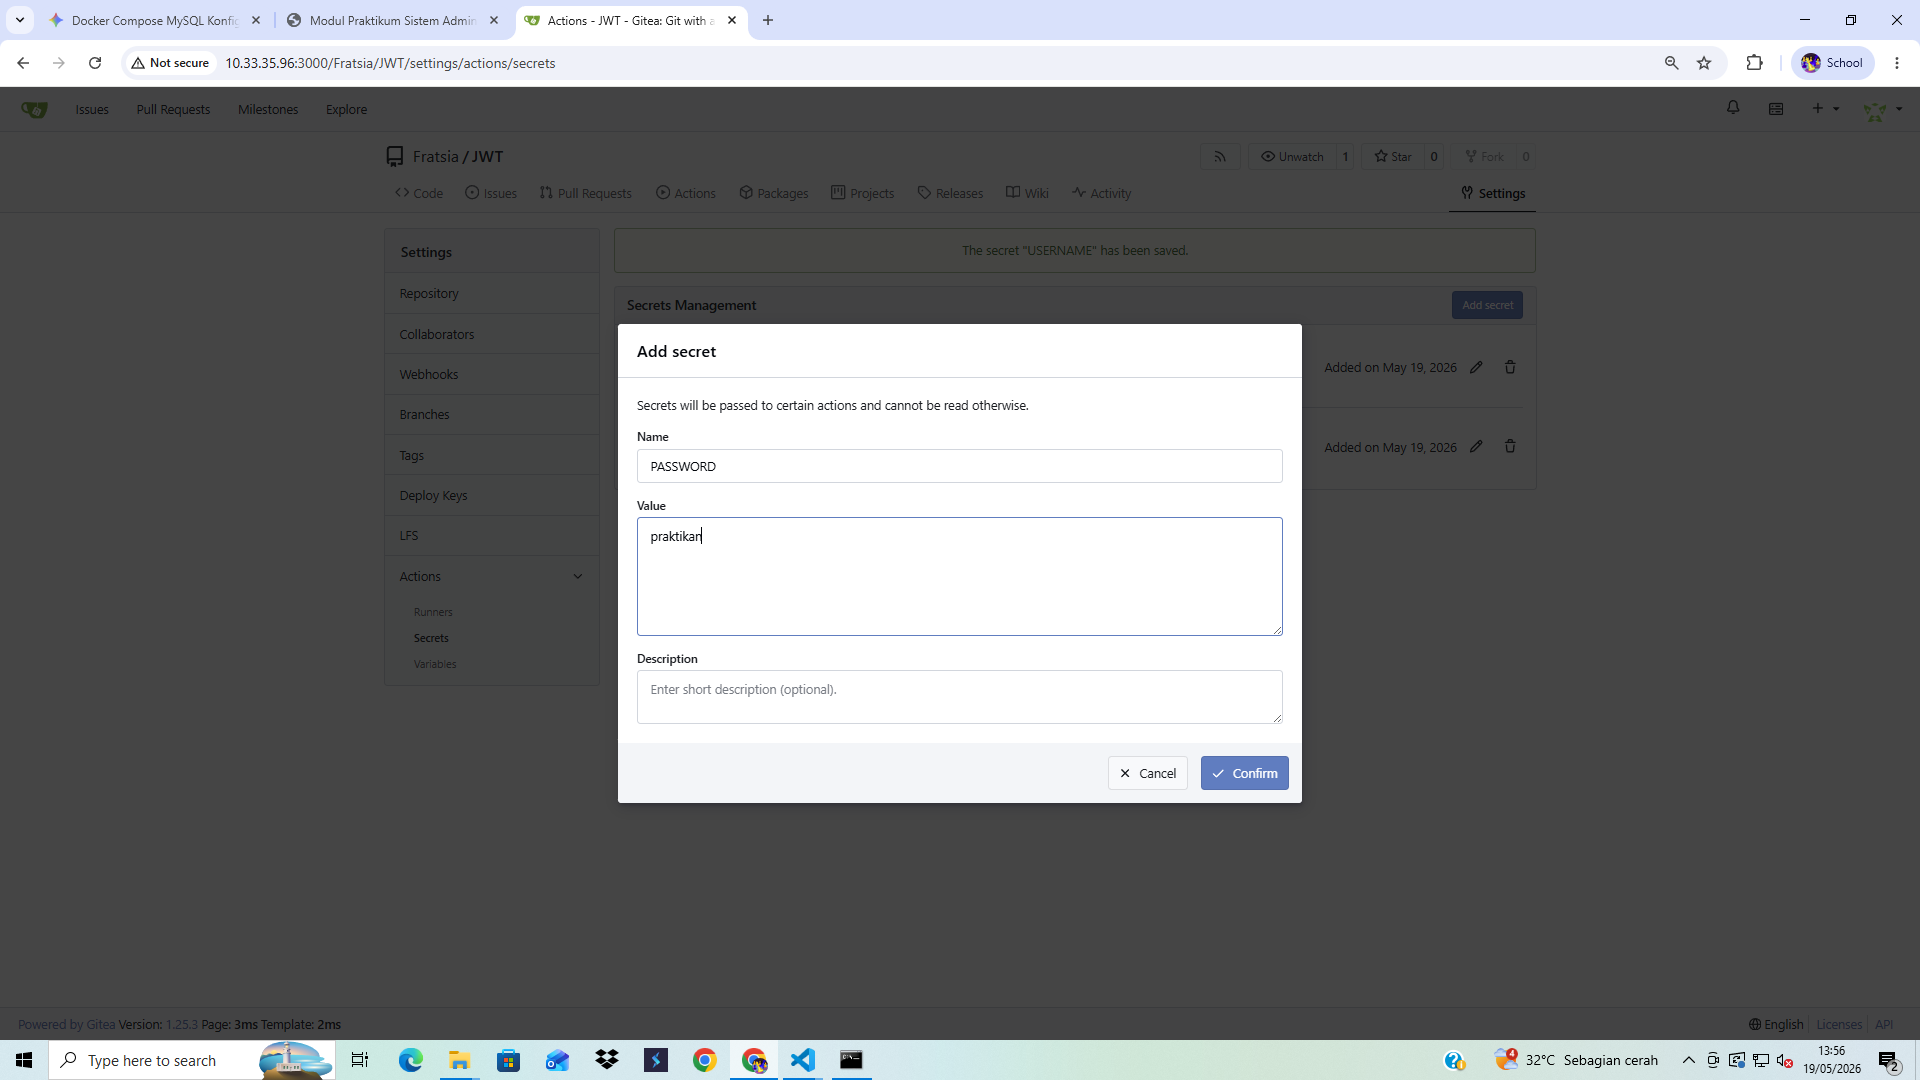
\includegraphics[width=0.95\textwidth]{resource/dokumentasi/26 - tambahkan secret password.png}
  \caption{Menambahkan Secret untuk \texttt{PASSWORD} SSH}
  \label{fig:p11-26-secret-pass}
\end{figure}

\subsection{Penambahan enpoint baru pada aplikasi untuk memudahkan verifikasi hasil deployment}

\par Sebelum melakukan pengujian otomatisasi deployment, saya menambahkan sebuah endpoint baru \texttt{/api/cicd} pada berkas \texttt{index.php} (Gambar \ref{fig:p11-27-route-cicd}). Endpoint ini berfungsi sebagai penanda visual untuk memverifikasi apakah pembaruan kode berhasil ter-deploy ke server setelah pipeline selesai dijalankan.

\begin{figure}[H]
  \centering
  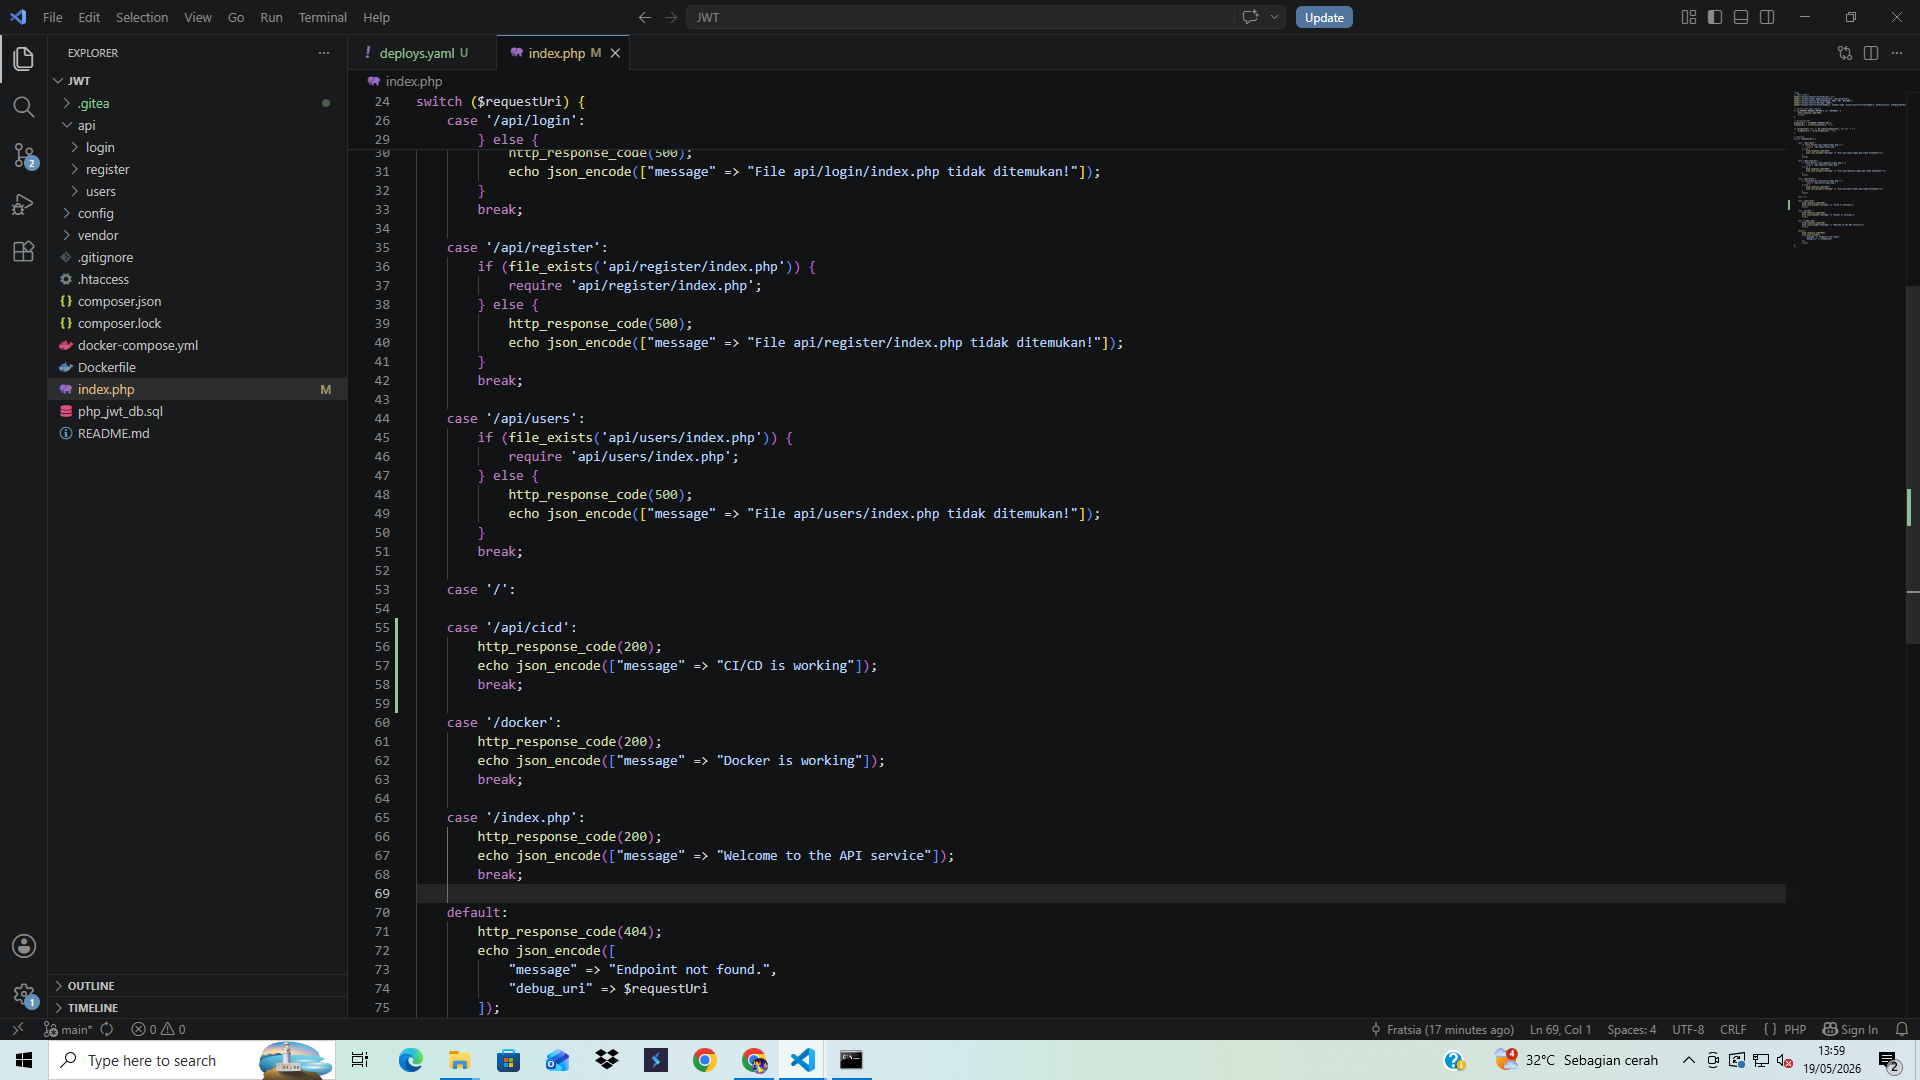
\includegraphics[width=0.95\textwidth]{resource/dokumentasi/27 - tambahkan route cicd.png}
  \caption{Menambahkan endpoint \texttt{/api/cicd} pada \texttt{index.php}}
  \label{fig:p11-27-route-cicd}
\end{figure}

\par Sebelum perubahan kode tersebut di-push ke Gitea, pengujian akses awal dilakukan ke alamat endpoint \texttt{/api/cicd} di web browser (Gambar \ref{fig:p11-28-cicd-notfound}). Hasilnya menunjukkan respons error \textit{Endpoint not found}, yang membuktikan bahwa endpoint baru tersebut belum aktif di server VPS sebelum sistem CI/CD memproses pembaruan.

\begin{figure}[H]
  \centering
  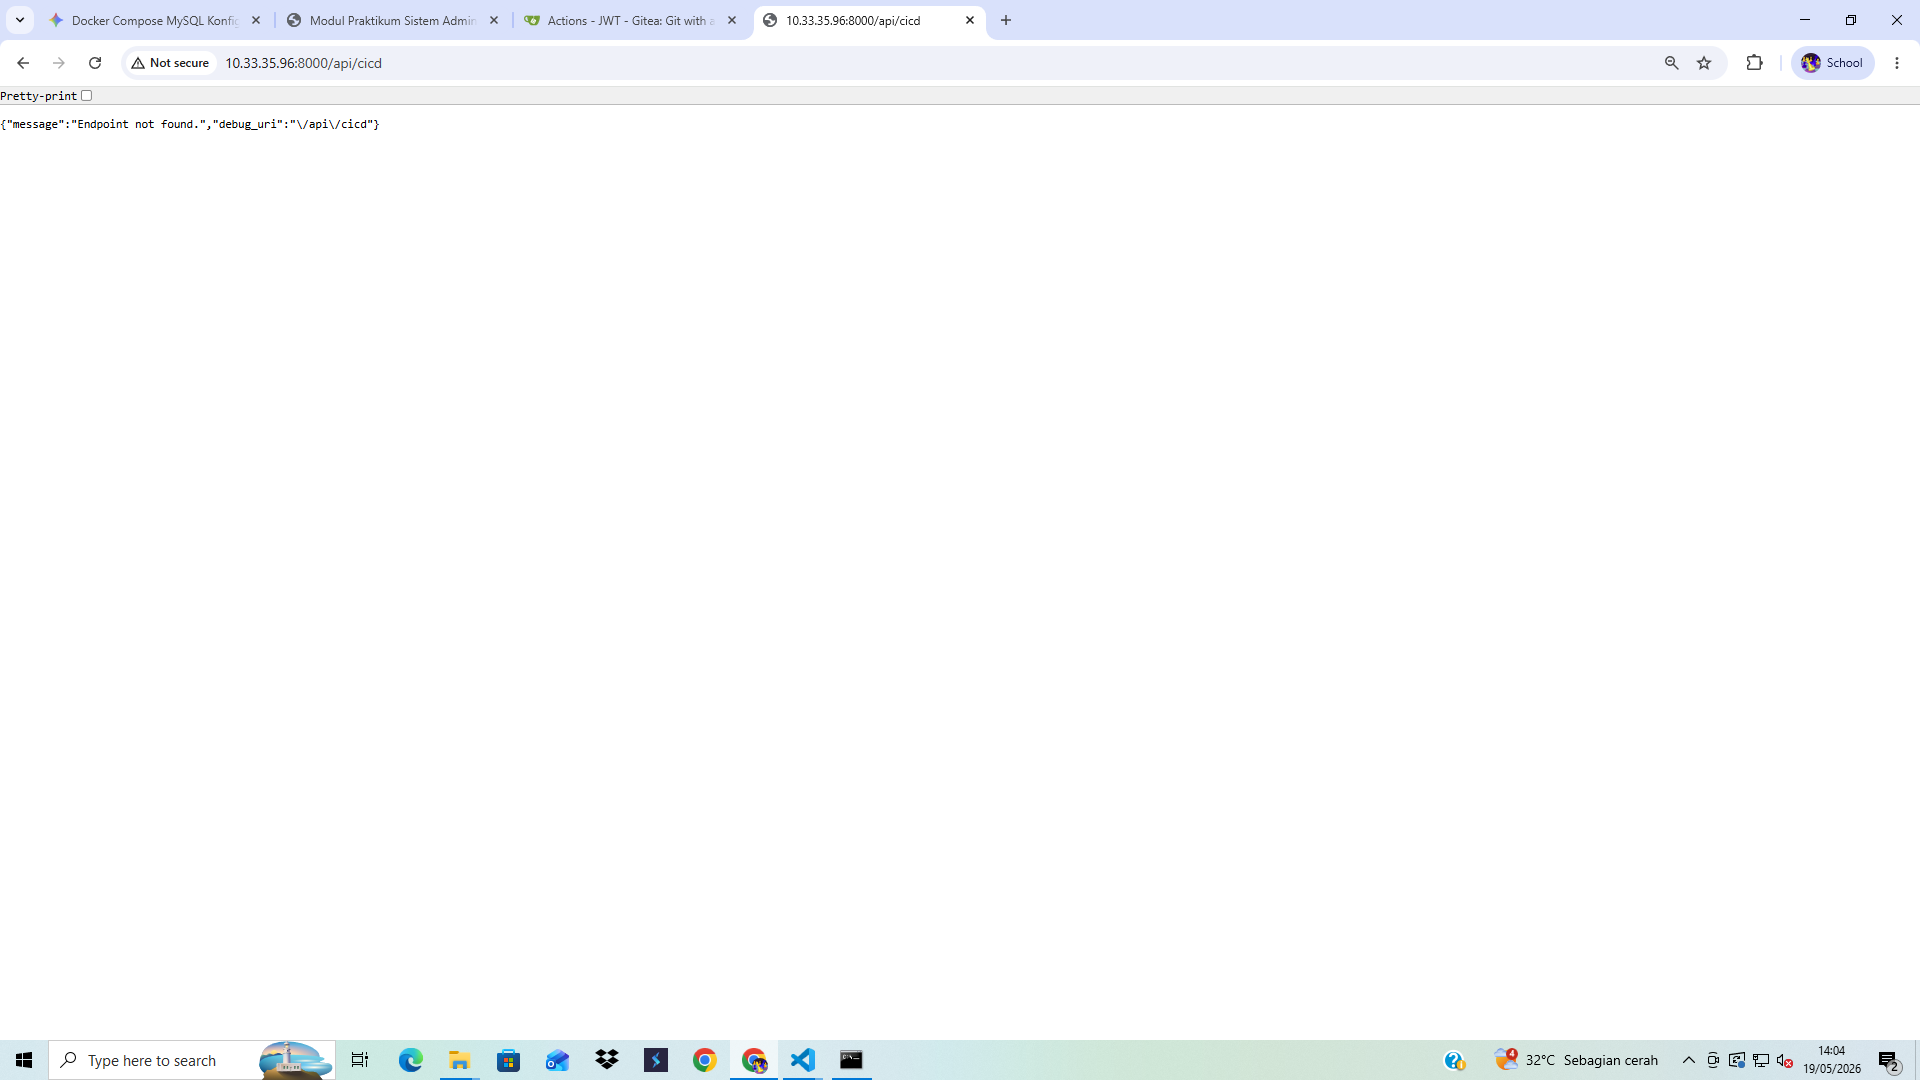
\includegraphics[width=0.95\textwidth]{resource/dokumentasi/28 - tidak ditemukan karena cicd belum di jalankan, belum di push.png}
  \caption{Endpoint \texttt{/api/cicd} belum tersedia sebelum deployment otomatis dilakukan}
  \label{fig:p11-28-cicd-notfound}
\end{figure}

\subsection{Push Aplikasi ke Gitea dan menjalankan pipeline untuk memverifikasi hasil deployment}

\par Setelah penambahan file workflow dan modifikasi kode selesai dilakukan, saya melakukan perintah \texttt{git add .}, \texttt{git commit}, dan \texttt{git push} untuk mengirimkan pembaruan tersebut ke repositori utama Gitea (Gambar \ref{fig:p11-29-push-app}). Jika diminta kredensial keamanan oleh sistem, autentikasi dilakukan menggunakan akun Gitea yang valid.

\begin{figure}[H]
  \centering
  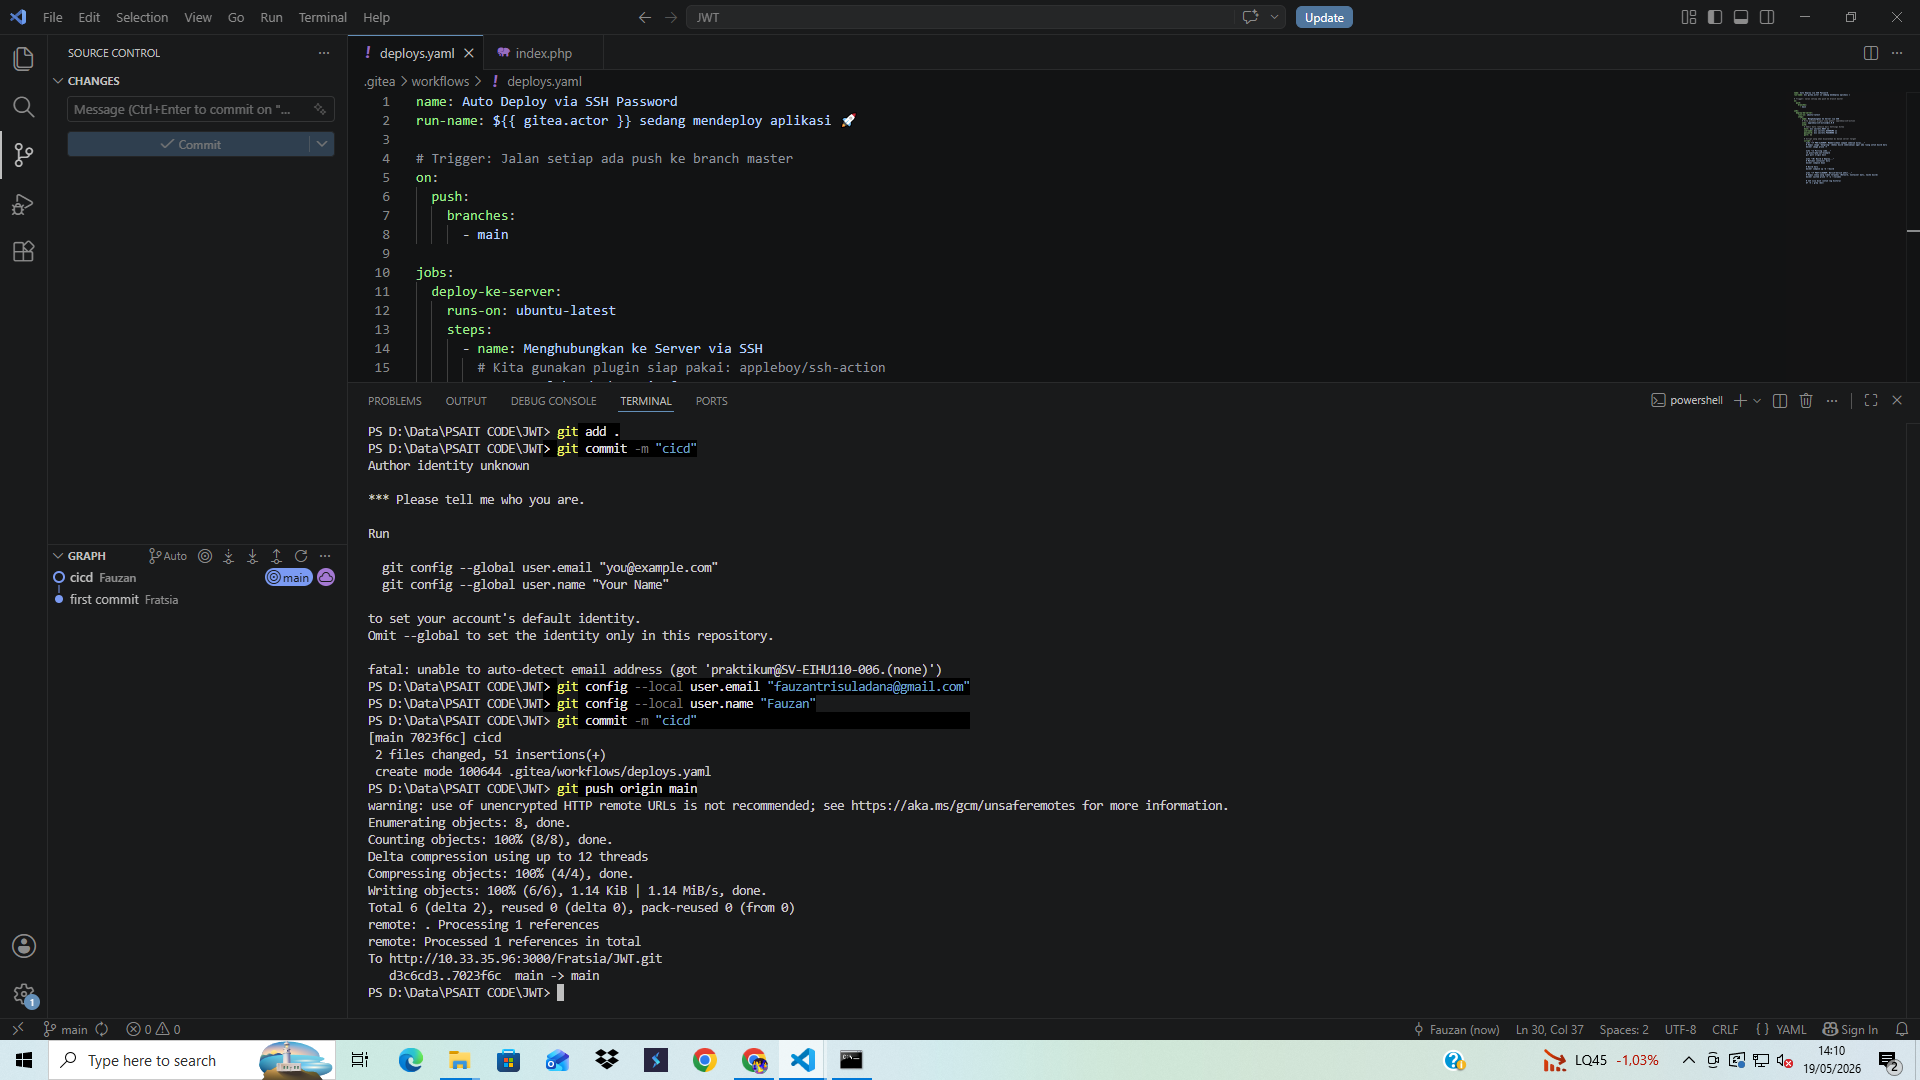
\includegraphics[width=0.95\textwidth]{resource/dokumentasi/29 - push aplikasi.png}
  \caption{Melakukan \textit{push} perubahan ke Gitea untuk memicu \textit{pipeline}}
  \label{fig:p11-29-push-app}
\end{figure}

\par Unggahan kode baru ke branch \texttt{main} secara otomatis memicu Gitea Actions untuk menjalankan pipeline deployment. Jalannya eksekusi dapat dipantau secara langsung melalui antarmuka Gitea Actions (Gambar \ref{fig:p11-30-gitea-action}). Gitea Runner bertindak sebagai agen pelaksana untuk masuk VPS secara otomatis, menarik perubahan kode terbaru, membangun container Docker baru, dan mematikan container lama.

\begin{figure}[H]
  \centering
  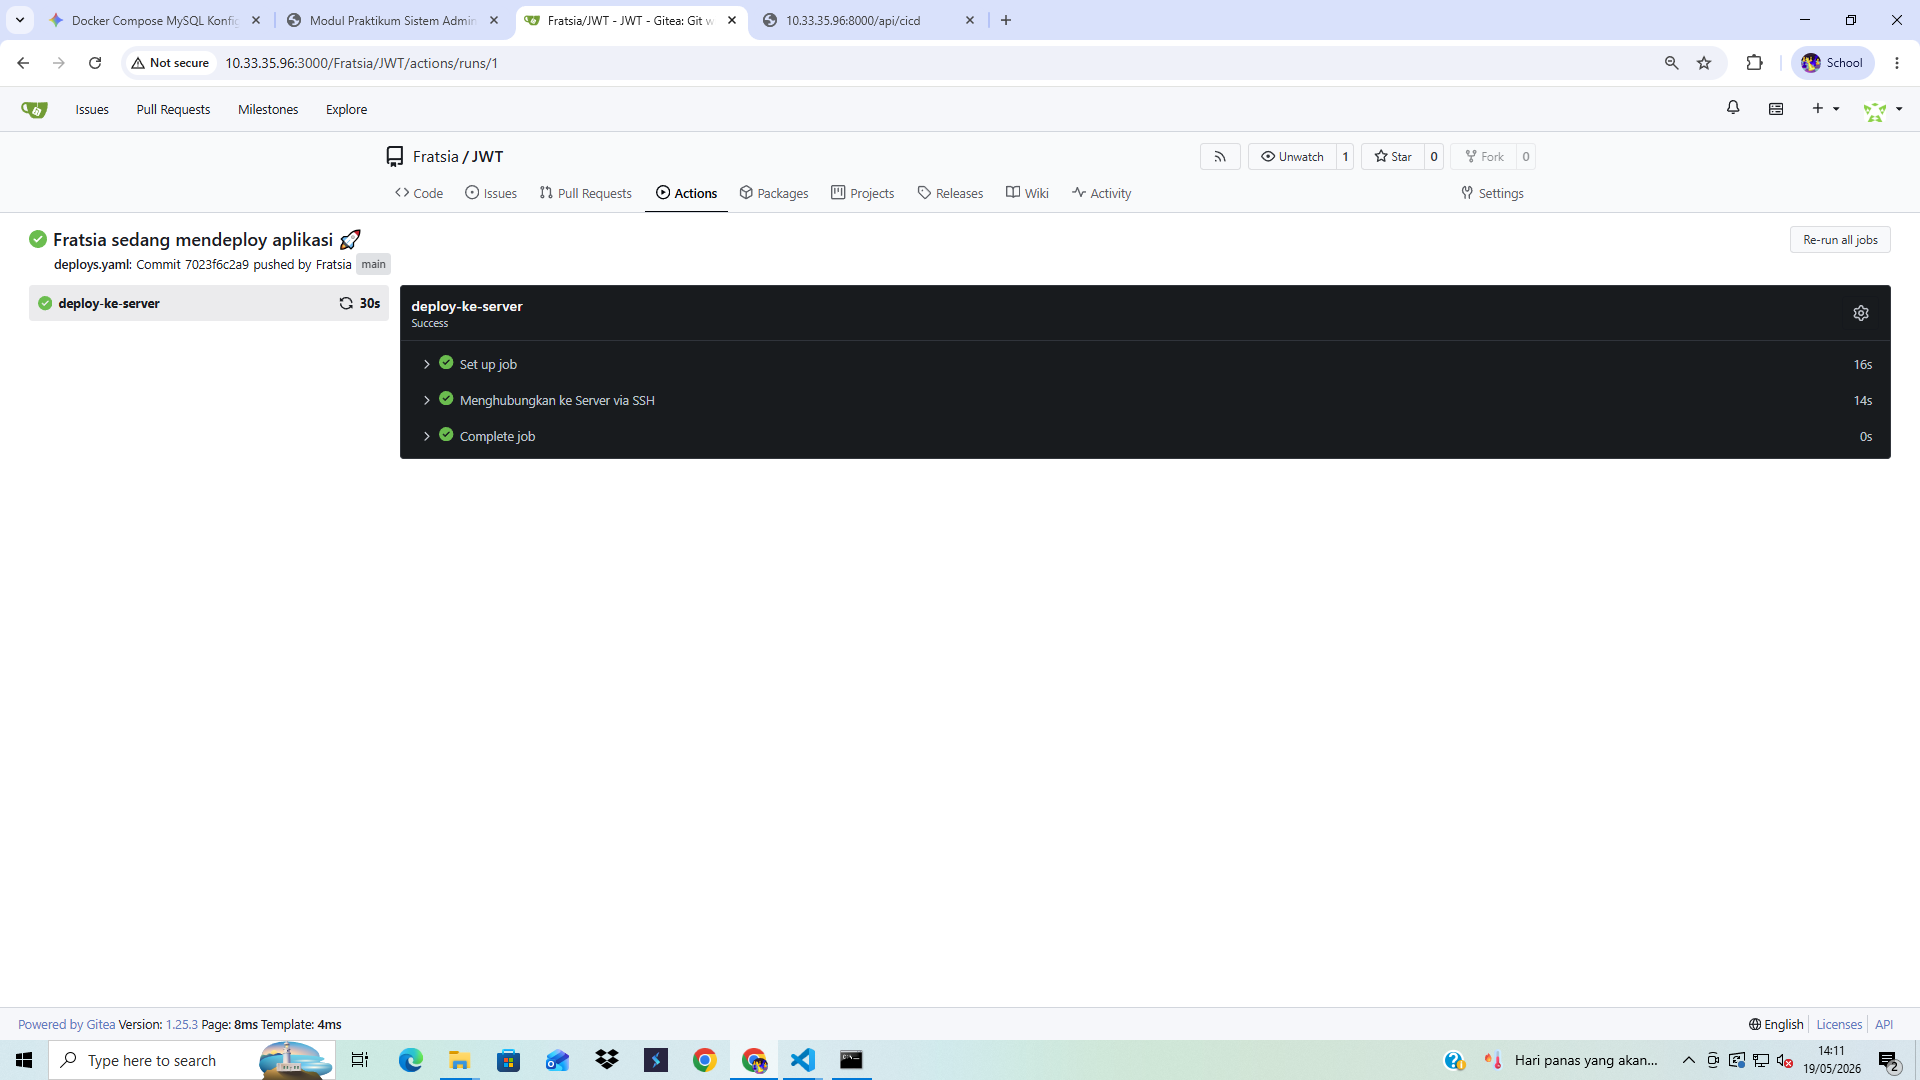
\includegraphics[width=0.95\textwidth]{resource/dokumentasi/30 - action di gitea.png}
  \caption{Proses eksekusi otomatis (\textit{workflow}) yang berjalan di Gitea Actions}
  \label{fig:p11-30-gitea-action}
\end{figure}

\subsection{Cek action CICD di aplikasi (enpoint baru).}

\par Setelah runner selesai memproses seluruh perintah dengan sukses (ditandai dengan indikator centang hijau pada riwayat aksi commit), pengujian verifikasi dilakukan dengan mengakses kembali URL endpoint \texttt{/api/cicd} di web browser. Pada Gambar \ref{fig:p11-31-cicd-working}, terlihat bahwa halaman web browser berhasil memuat respons sukses dalam format JSON yang dikirimkan oleh server VPS. Hal ini menunjukkan bahwa pembaruan kode aplikasi telah berhasil diterapkan secara otomatis melalui alur CI/CD tanpa intervensi manual tambahan di sisi server.

\begin{figure}[H]
  \centering
  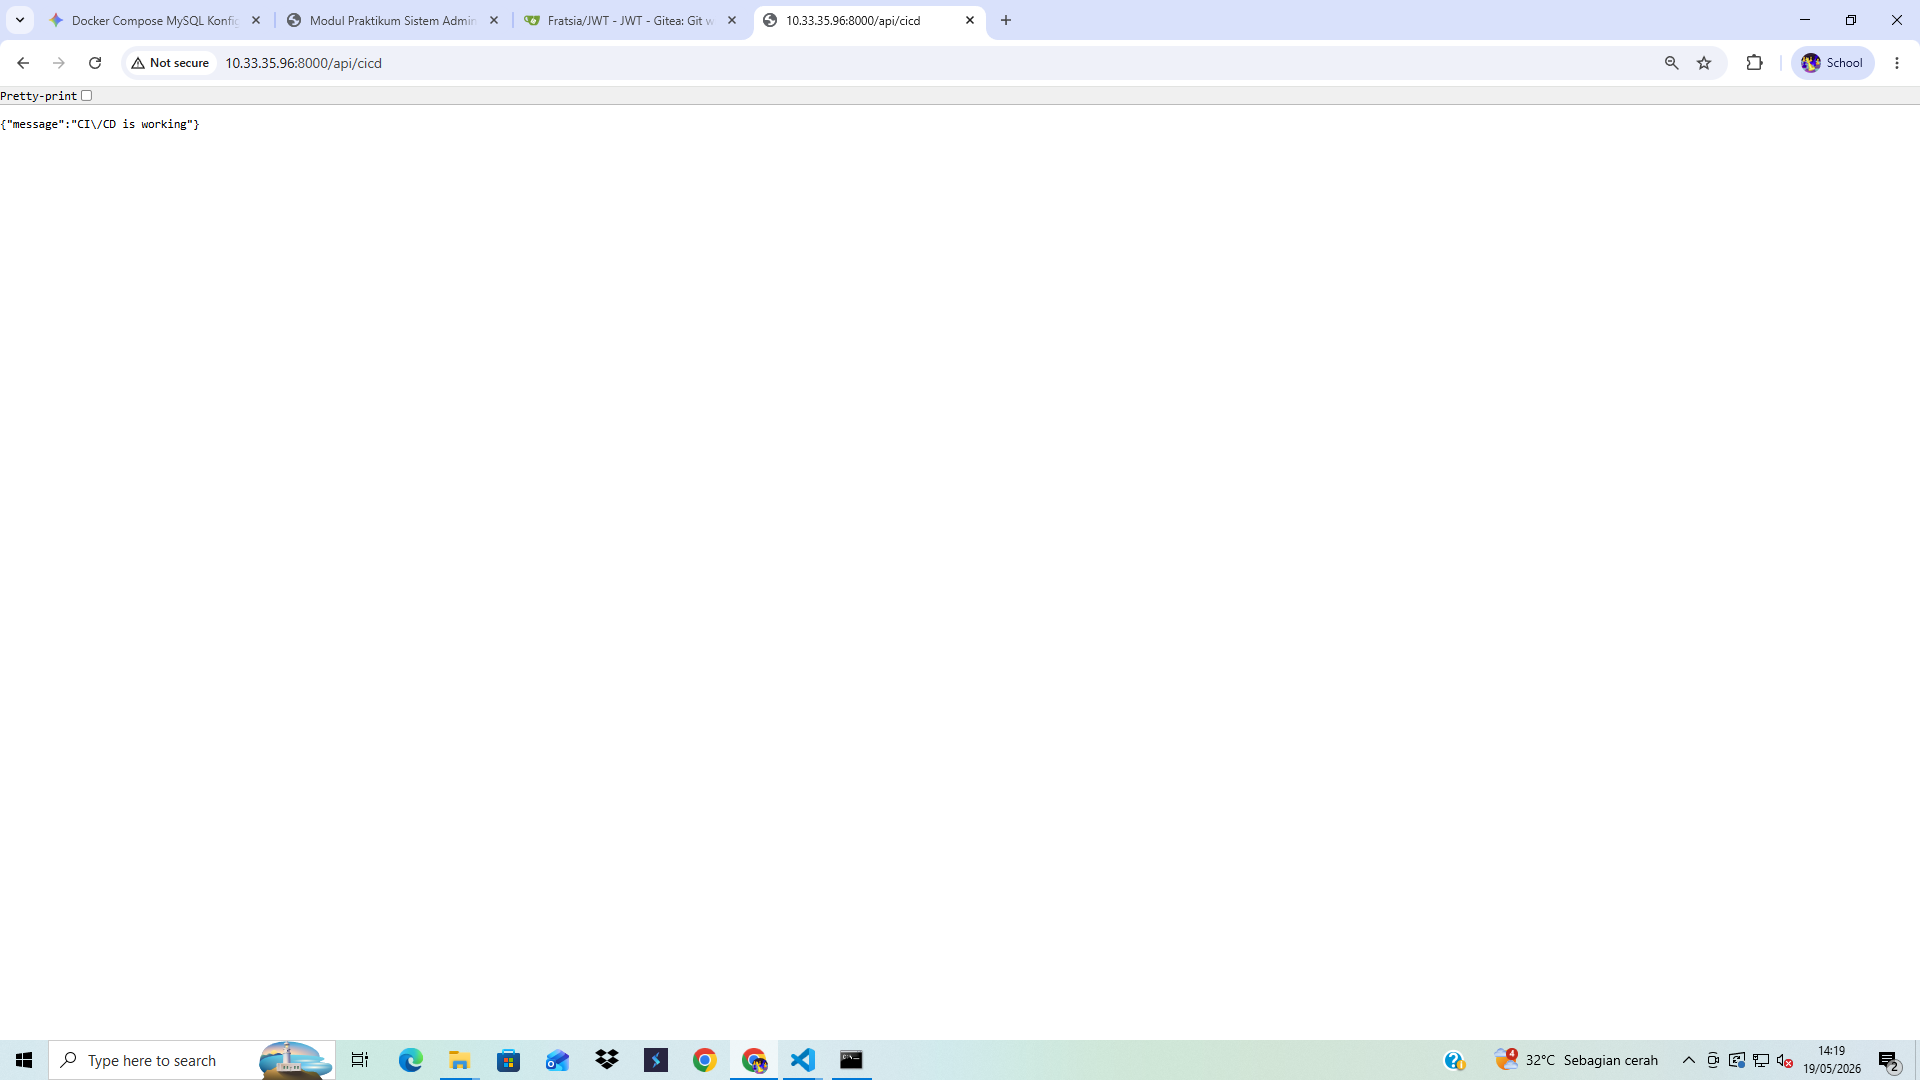
\includegraphics[width=0.95\textwidth]{resource/dokumentasi/31 - cicd working.png}
  \caption{Aplikasi berhasil diperbarui, endpoint \texttt{/api/cicd} mengembalikan respons JSON sukses}
  \label{fig:p11-31-cicd-working}
\end{figure}

\subsection{Pengerjaan Tugas}
\par Selanjutnya saya mengerjakan dua tugas tambahan. Tugas pertama berfokus pada perubahan logika program, sedangkan tugas kedua berfokus pada pembuktian bahwa perubahan pada kode sumber dapat memicu deployment otomatis melalui Gitea Actions.

\subsubsection{Tugas 1}
\par Pada tugas pertama, saya mengubah nilai pada pengujian matematika sederhana agar pipeline dapat divalidasi dari hasil keluaran yang benar. Proses pengujian awal ditunjukkan pada Gambar \ref{fig:p11-32-test-matematika}. Setelah itu, saya melakukan perubahan pada kode deployment dan melakukan \textit{push} ke repository seperti pada Gambar \ref{fig:p11-33-change-push}. Perubahan tersebut kemudian memicu eksekusi workflow di Gitea Actions, yang ditunjukkan pada Gambar \ref{fig:p11-34-run-action}.

\begin{figure}[H]
  \centering
  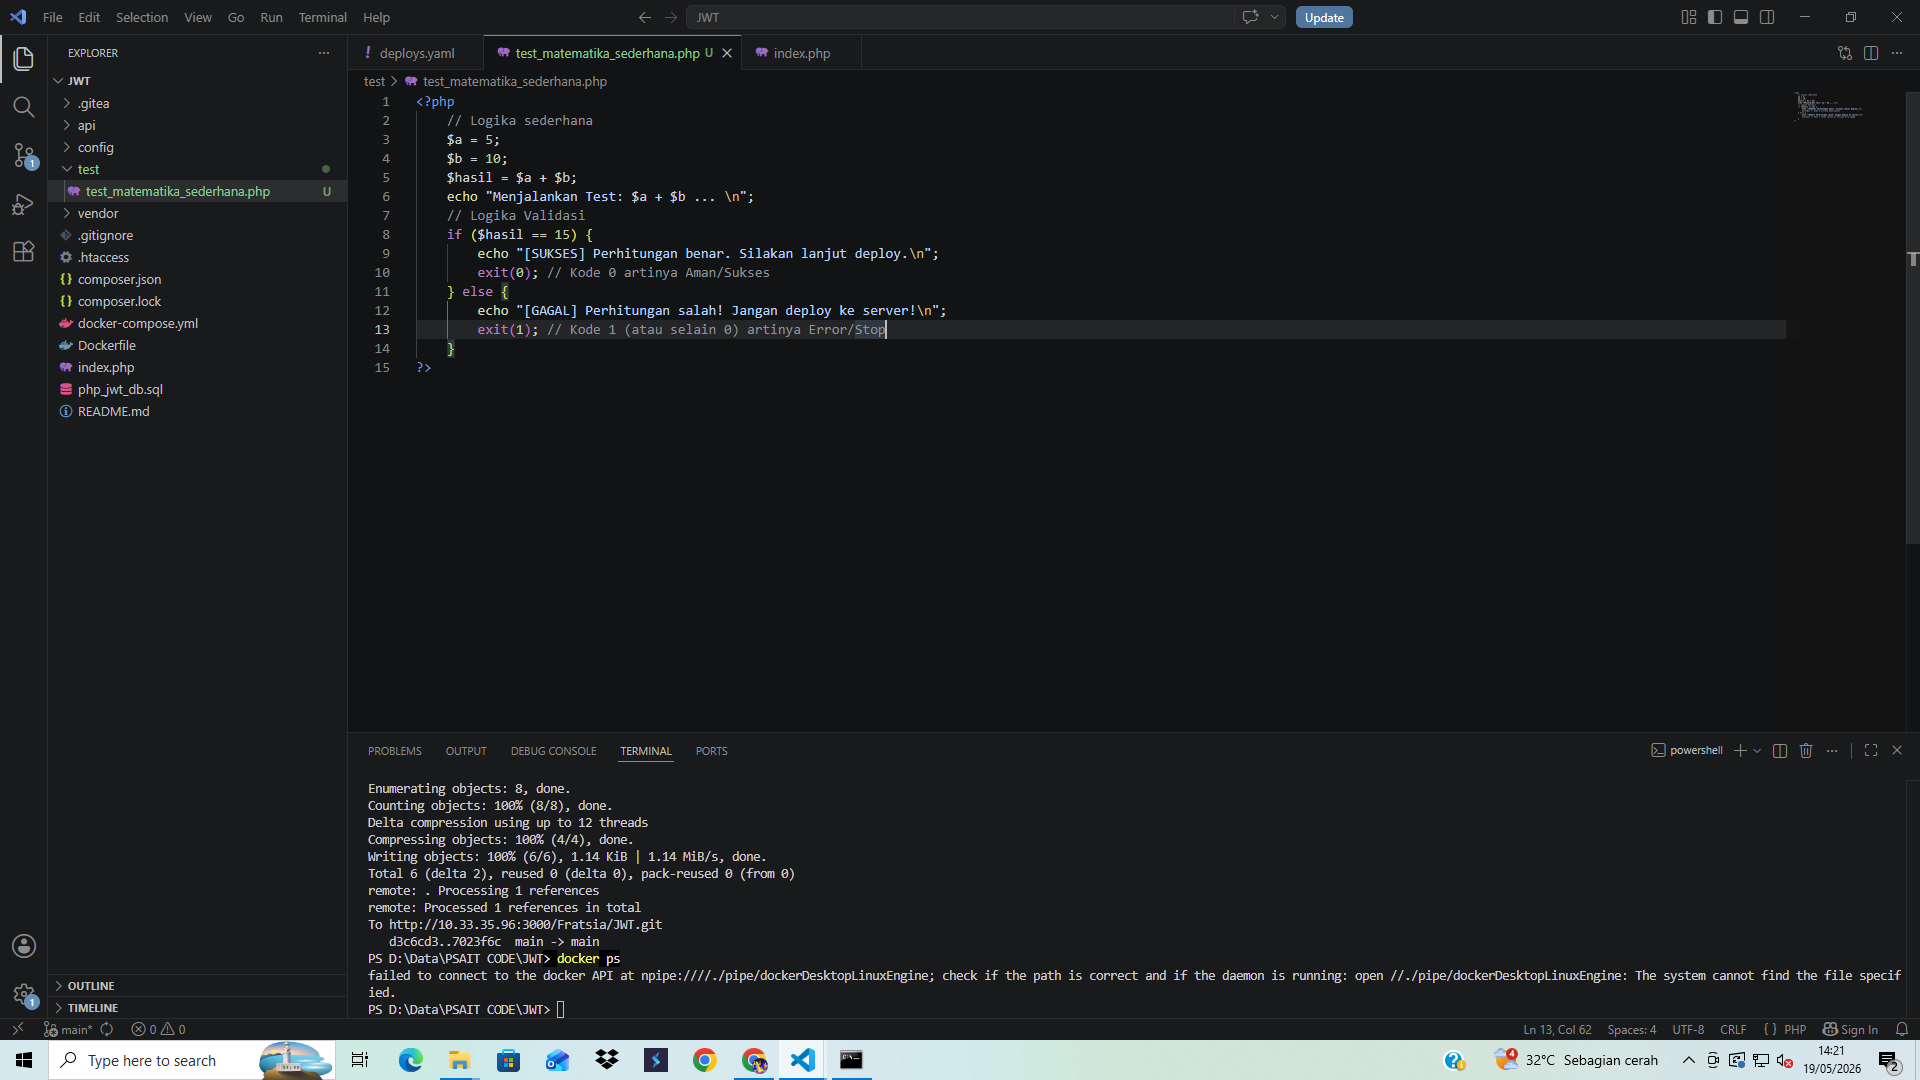
\includegraphics[width=0.95\textwidth]{resource/dokumentasi/32 - Tugas 1 - test matematika.png}
  \caption{Pengujian awal untuk tugas 1 dengan hasil perhitungan matematika sederhana}
  \label{fig:p11-32-test-matematika}
\end{figure}

\begin{figure}[H]
  \centering
  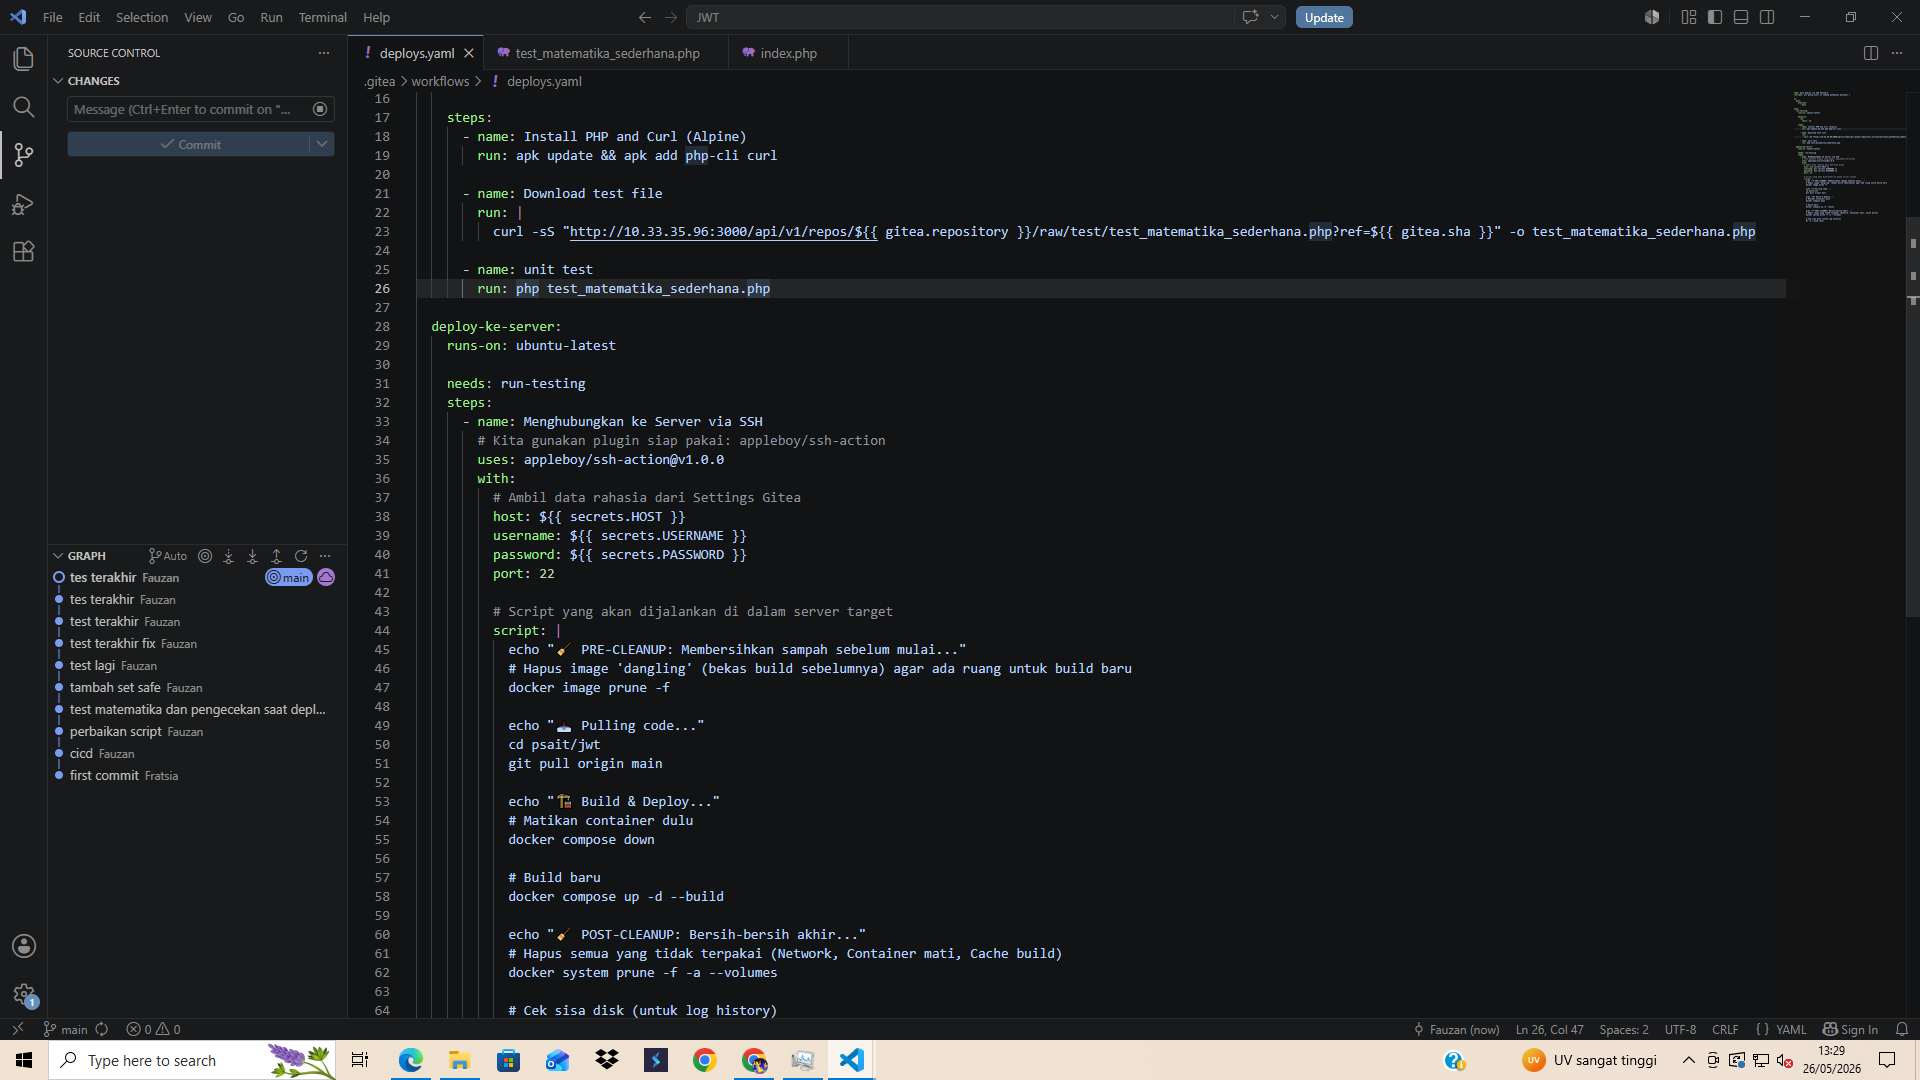
\includegraphics[width=0.95\textwidth]{resource/dokumentasi/33 - Tugas 1 - perubahan kode deploy dan git push.png}
  \caption{Perubahan kode deployment dan proses \textit{git push} pada tugas 1}
  \label{fig:p11-33-change-push}
\end{figure}

\begin{figure}[H]
  \centering
  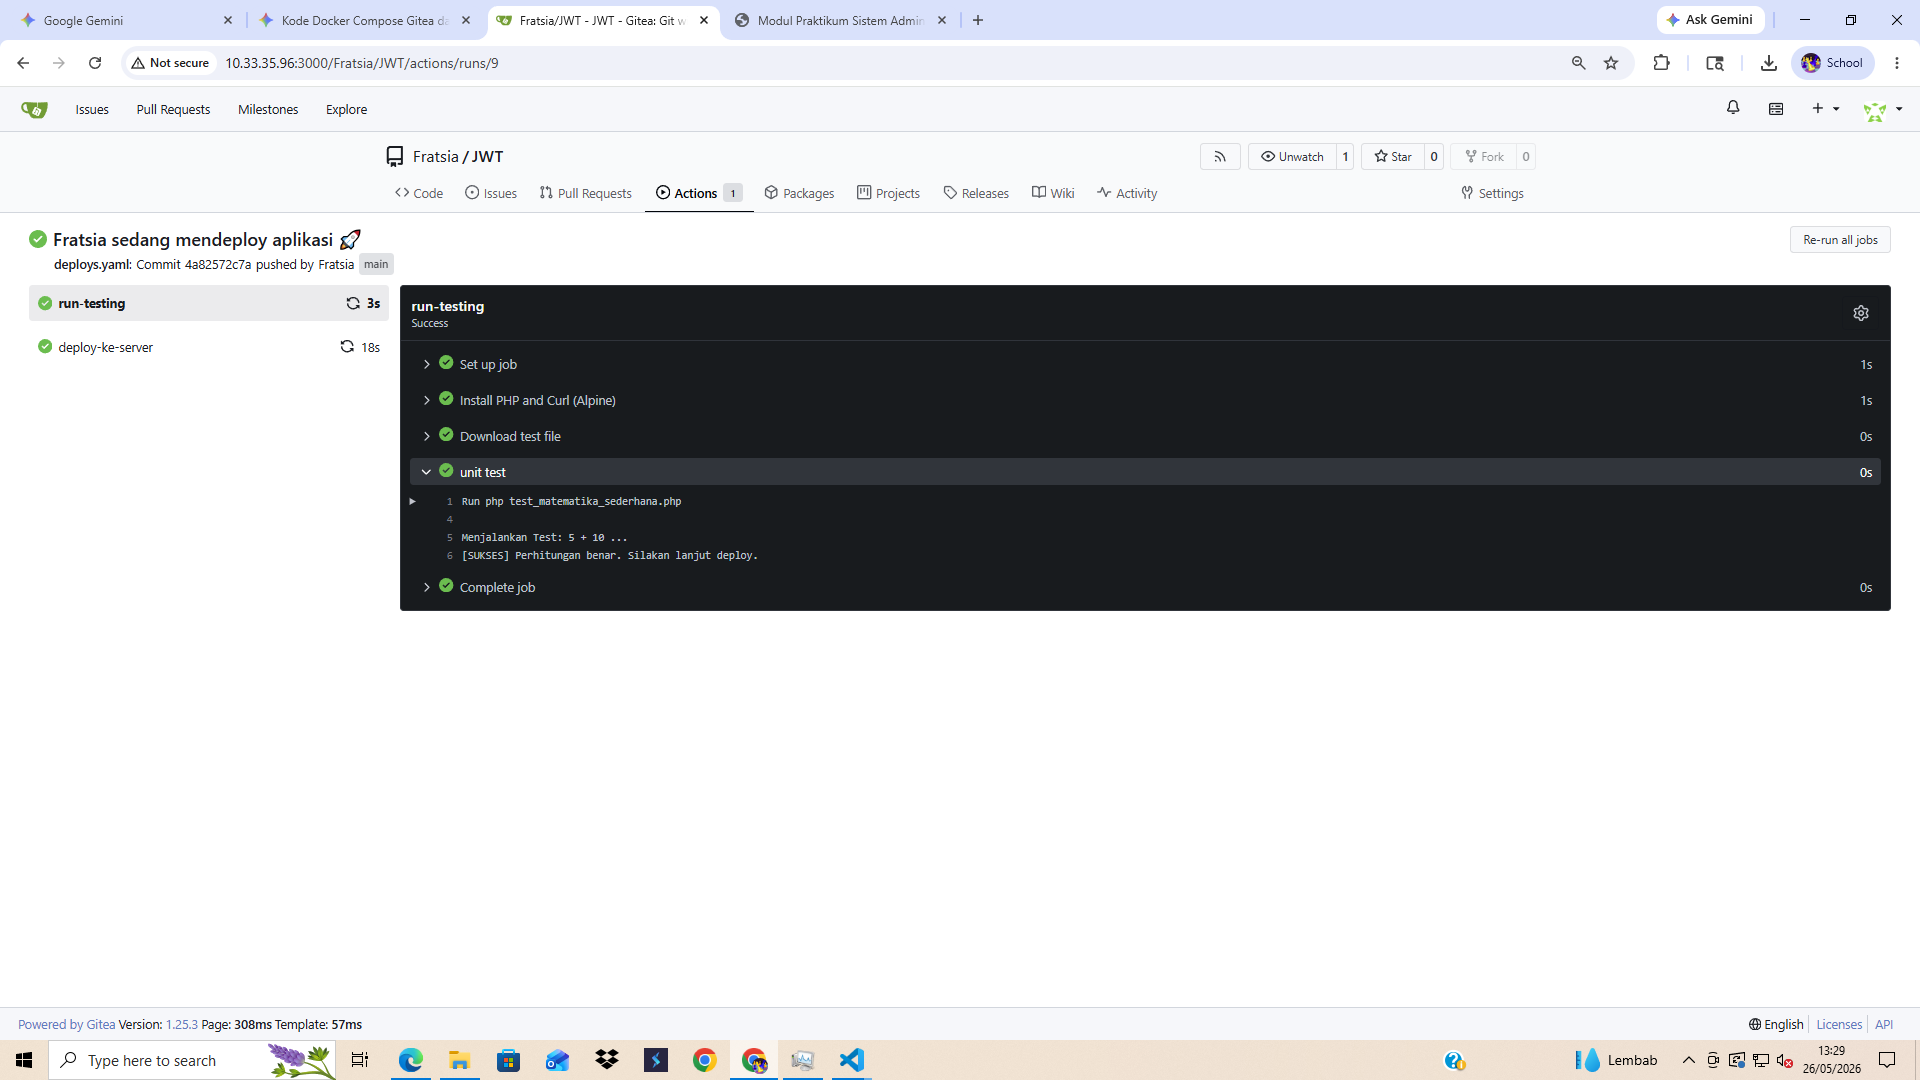
\includegraphics[width=0.95\textwidth]{resource/dokumentasi/34 - Tugas 1 - Run action di gitea.png}
  \caption{Workflow Gitea Actions berjalan setelah perubahan pada tugas 1}
  \label{fig:p11-34-run-action}
\end{figure}

\subsubsection{Tugas 2}
\par Pada tugas kedua, saya mengubah hasil pengujian agar memastikan pipeline kembali berjalan dari awal hingga akhir. Hasil perubahan terlihat pada Gambar \ref{fig:p11-35-change-test}. Setelah kode diperbarui, workflow dijalankan kembali melalui Gitea Actions seperti pada Gambar \ref{fig:p11-36-run-action}.

\begin{figure}[H]
  \centering
  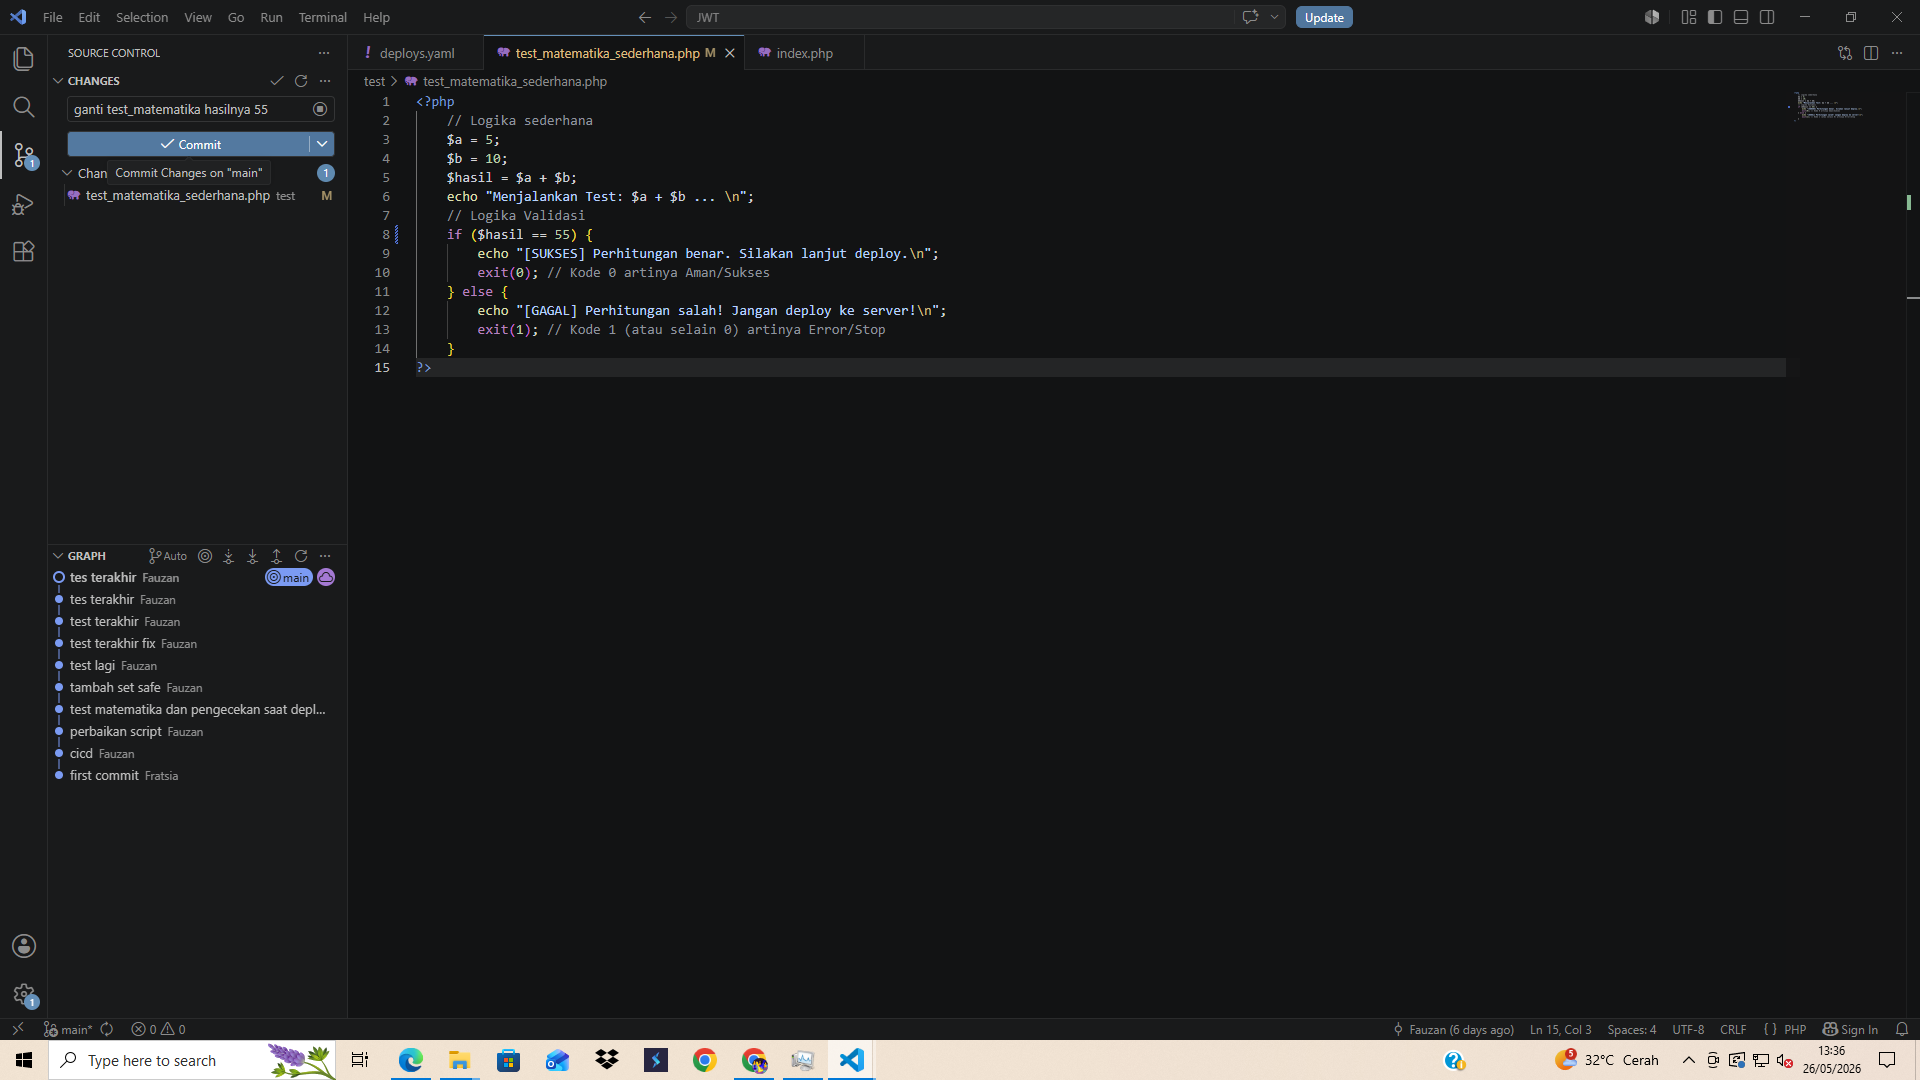
\includegraphics[width=0.95\textwidth]{resource/dokumentasi/35 - Tugas 2 - mengubah hasil di tes.png}
  \caption{Perubahan hasil pengujian pada tugas 2}
  \label{fig:p11-35-change-test}
\end{figure}

\begin{figure}[H]
  \centering
  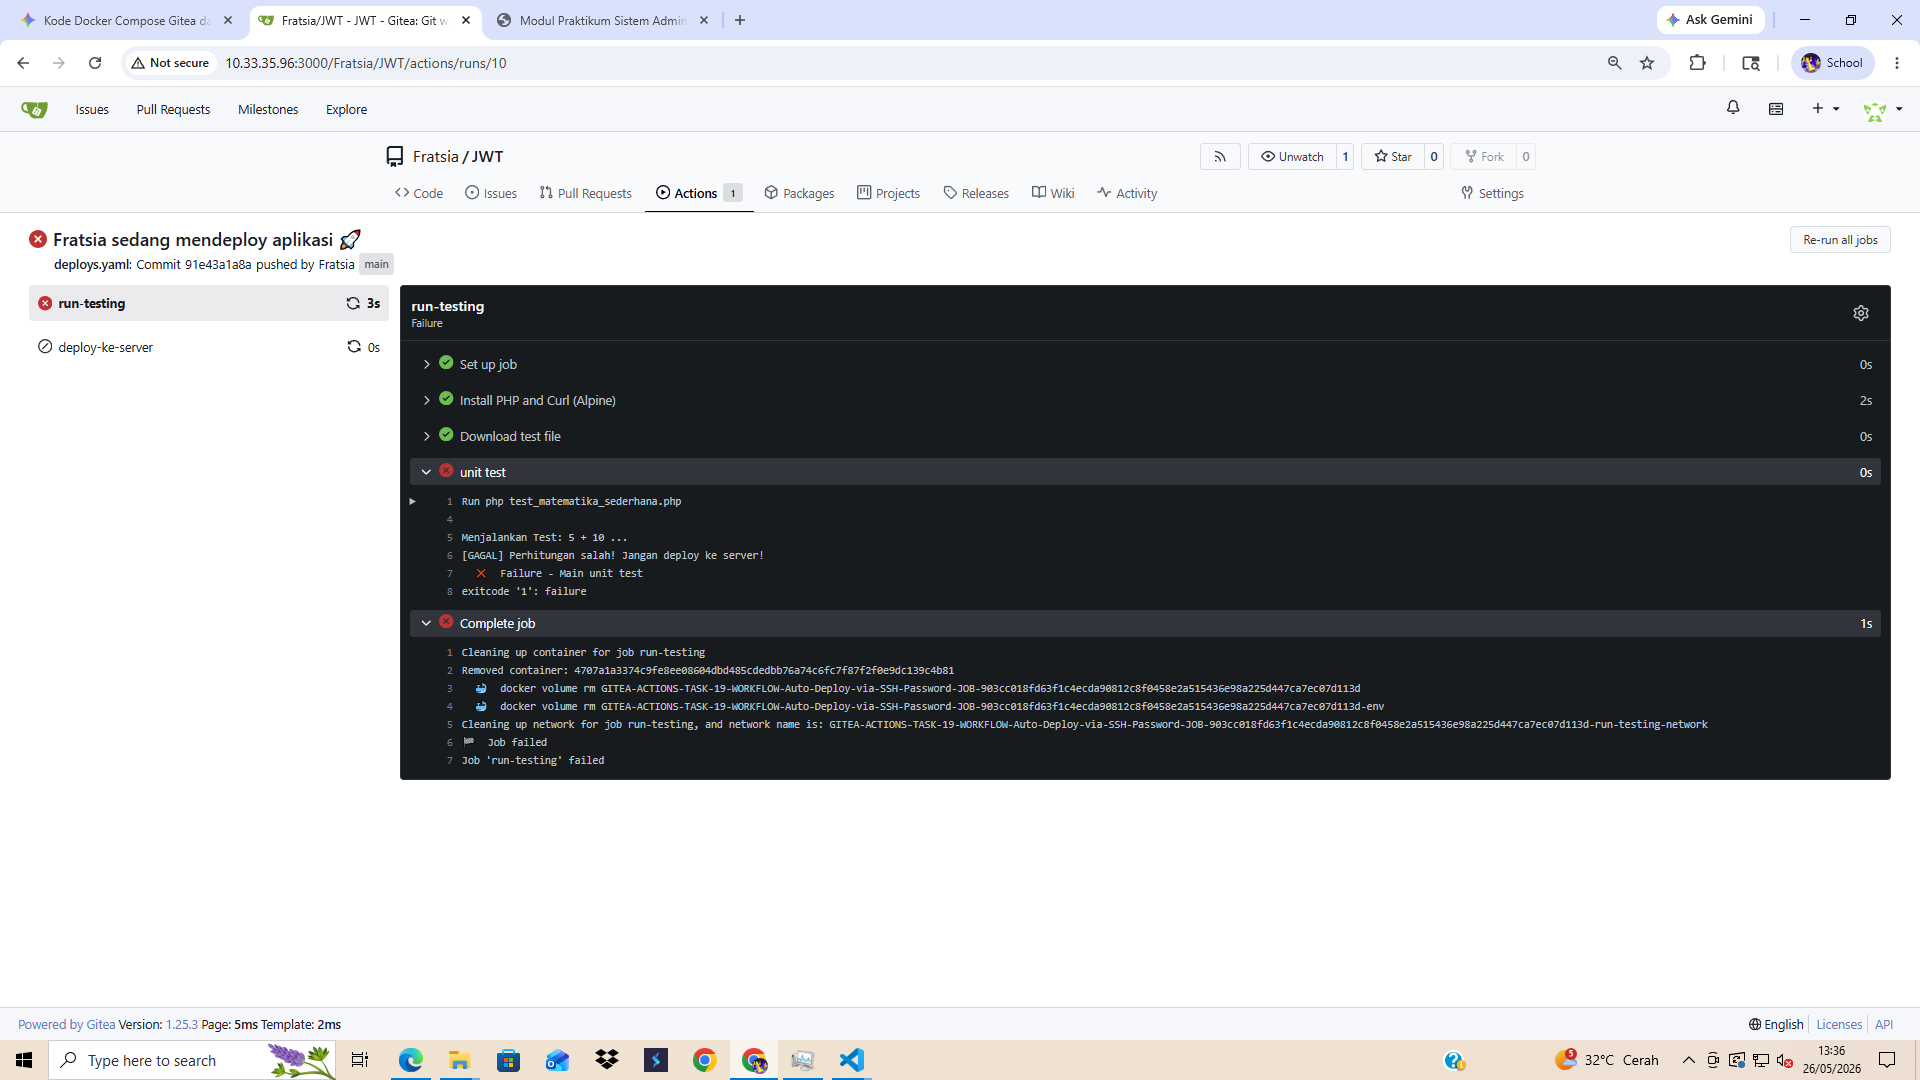
\includegraphics[width=0.95\textwidth]{resource/dokumentasi/36 - Tugas 2 - Run action di gitea.png}
  \caption{Workflow Gitea Actions dijalankan kembali pada tugas 2}
  \label{fig:p11-36-run-action}
\end{figure}

\section{Kesimpulan}

\par Kesimpulan dari praktikum \textit{Ci/Cd Pipeline Lokal dengan Gitea Action} adalah sebagai berikut:
\begin{enumerate}
  \item Infrastruktur CI/CD pipeline lokal berhasil diimplementasikan secara mandiri (\textit{self-hosted}) menggunakan kombinasi layanan Git Gitea dan Gitea Runner di atas server VPS.
  \item Konfigurasi variabel environment database yang disesuaikan ke IP VPS host memastikan container aplikasi API tetap dapat terhubung secara lancar ke database MySQL yang berjalan di luar jaringan Docker Compose aplikasi.
  \item Berkas workflow \texttt{deploys.yaml} yang ditempatkan di direktori \texttt{.gitea/workflows/} berhasil mengotomatiskan proses penarikan kode (\textit{git pull}), rebuild container (\texttt{docker compose up -d --build}), serta pembersihan berkas sampah Docker secara terjadwal setiap ada aktivitas push di branch \texttt{main}.
  \item Fitur Gitea Secrets terbukti efektif untuk mengamankan data kredensial akses SSH ke server VPS (\texttt{HOST}, \texttt{USERNAME}, dan \texttt{PASSWORD}) dari paparan repositori publik.
  \item Endpoint verifikasi \texttt{/api/cicd} mempermudah proses validasi hasil deployment otomatis secara instan melalui web browser pasca-pipeline selesai dijalankan.
  \item Pengujian tugas matematika membuktikan bahwa Gitea Runner mampu memvalidasi kelayakan kode dan membatalkan alur deployment secara otomatis jika terdeteksi kegagalan logika pada tahapan pengujian.
\end{enumerate}

\section{Daftar Pustaka}
\printbibliography[heading=none]

\end{document}